\documentclass[range]{ar2e}%%%Put [range] option here for references citations to
                           %%%print as [1--10] for numbered references.
                           %%% Default is [1,2,3,4,5,6,7,8,9,10]
                           
\usepackage{graphicx}
\usepackage{lineno}
%\usepackage{cite}
\bibliographystyle{arnuke_revised}

% imported
\newcommand{\be}{\begin{equation}}
\newcommand{\ee}{\end{equation}}
\newcommand{\bea}{\begin{eqnarray}}
\newcommand{\eea}{\end{eqnarray}}
\newcommand{\nn}{\nonumber}
\newcommand{\pT}{\mbox{$p_{\mathrm{T}}$}}
\newcommand{\vtwo}{\mbox{$v_2$}}
\newcommand{\energy}{\mbox{$\sqrt{s_{\mathrm{NN}}}$}}

% GR's macros
\newcommand{\dd}{\mbox{$\mathrm{d}$}}
%\newcommand{\pp}{\mbox{$pp$}}
\newcommand{\AuAu}{\mbox{Au+Au}}
\newcommand{\PbPb}{\mbox{Pb+Pb}}
\newcommand{\Ncoll}{\mbox{$N_{\mathrm{coll}}$}}
\newcommand{\Npart}{\mbox{$N_{\mathrm{part}}$}}
\newcommand{\TAAb}{\mbox{$T_{\mathrm{AA}}(b)$}}
\newcommand{\Rcp}{\mbox{$R_{\rm CP}$}}
\newcommand{\RFour}{\mbox{$R = 0.4$}}
\newcommand{\RcpRatio}{\mbox{$R_{\mathrm{CP}}^{R}/R_{\mathrm{CP}}^{\,0.2}$}}
\newcommand{\kt}{\mbox{$k_{t}$}}
\newcommand{\antikt}{\mbox{anti-\kt}}
\newcommand{\sumet}{\mbox{$\Sigma E_{\mathrm{T}}$}}
\newcommand{\Nevt}{\mbox{$N_{\mathrm{evt}}$}}
\newcommand{\vtjet}{\mbox{$v_2^{\mathrm{jet}}$}}
\newcommand{\Dphi}{\mbox{$\Delta \varphi$}}

\newcommand{\text}{\mbox}
\providecommand{\rd}{\mathrm{d}}
\newcommand {\lum}    {\ensuremath{150\,\mu\mathrm{b}^{-1}}}
\newcommand {\roots}    {\ensuremath{\sqrt{s}}}
\newcommand {\rootsNN}  {\ensuremath{\sqrt{s_{_{\rm NN}}}}}
\newcommand {\sqrtsnn}  {\ensuremath{\sqrt{s_{_{\rm NN}}}}}
\newcommand {\dndy}     {\ensuremath{{\rd}N/{\rd}y}}
\newcommand {\dnchdy}   {\ensuremath{{\rd}N_{\text{ch}}/{\rd}y}}
\newcommand {\dndeta}   {\ensuremath{{\rd}N/{\rd}\eta}}
\newcommand {\dnchdeta} {\ensuremath{{\rd}N_{\text{ch}}/{\rd}\eta}}
\newcommand {\dndpt}    {\ensuremath{{\rd}N/{\rd}\pt}}
\newcommand {\dnchdpt}  {\ensuremath{{\rd}N_{\text{ch}}/{\rd}\pt}}
\newcommand {\deta}     {\ensuremath{\Delta\eta}}
\newcommand {\dphi}     {\ensuremath{\Delta\varphi_{1,2}}}
\newcommand {\AJ}       {\ensuremath{A_J}}
\newcommand {\npart}    {\ensuremath{N_{\text{part}}}}
\newcommand {\ncoll}    {\ensuremath{N_{\text{coll}}}}

\newcommand {\pp}    {\mbox{p+p}}
\newcommand {\ak} {anti-$k_\text{T}$}
\newcommand {\ptlead} {\ensuremath{p_{\rm{T},1}}}
\newcommand {\ptsub} {\ensuremath{p_{\rm{T},2}}}
\newcommand {\ptrat} {\ensuremath{\ptsub/\ptlead}}

\newcommand {\tev}       {\ensuremath{\,\mathrm{TeV}}}
\newcommand {\TeV}       {\ensuremath{\,\mathrm{TeV}}}
\newcommand {\GeV}       {\ensuremath{\,\mathrm{GeV}}}
\newcommand {\GeVc}      {\ensuremath{\,\mathrm{GeV}}}
\newcommand{\stat}{\ensuremath{\,\text{(stat.)}}}
\newcommand{\syst}{\ensuremath{\,\text{(syst.)}}}

\newcommand{\m}{\ensuremath{\,\text{m}}}
\providecommand{\mb}{\mbox{\,\mathrm{mb}}}
\providecommand{\nb}{\mbox{\,\mathrm{mb}}}
\newcommand {\naive}    {na\"{\i}ve}
\newcommand{\PHOJET} {{\sc{phojet}}}
\newcommand{\HYDJET}{{\sc{hydjet}}}
\newcommand{\PYTHYD}{{\sc{pythia+hydjet}}}
\newcommand{\PYTHIA}{{\sc{pythia}}}
\newcommand {\photonjet}{photon+jet}
\newcommand{\Pgpz}{\ensuremath{\pi^0}}
\newcommand{\Pgh}{\ensuremath{\eta}}
\newcommand{\Pgg}{\ensuremath{\gamma}}
\newcommand{\cPqb}{\ensuremath{b}}

\newcommand {\ptg}    {\ensuremath{p_{\mathrm{T}}^{\Pgg}}}
\newcommand {\ptj}    {\ensuremath{p_{\mathrm{T}}^{\text{jet}}}}
\newcommand {\phig}    {\ensuremath{\varphi^\Pgg}}
\newcommand {\phij}    {\ensuremath{\varphi^\mathrm{jet}}}

\providecommand{\ptjet}{\ptj}
\providecommand{\ptgamma}{\ptg}
\providecommand{\ptphoton}{\ptg}
\providecommand{\rjg}{\ensuremath{R_{J\Pgg}}}
\providecommand{\xjg}{\ensuremath{x_{J\Pgg}}}
\providecommand{\sjg}{\ensuremath{\sigma(\Delta\varphi_{J\Pgg})}}
\providecommand{\ptg}{\ensuremath{p_{\mathrm{T},\Pgg}}}
\providecommand{\dphijg}{\ensuremath{\Delta\varphi_{J\Pgg}}}
\providecommand{\avexjg}{\ensuremath{\langle x_{J\Pgg}\rangle}}
\providecommand{\sigeta}{\ensuremath{\sigma_{\eta\eta}}}

\providecommand {\mubinv}{\ensuremath{\mathrm{\mu b^{-1}}}}
\providecommand {\nbinv}{\ensuremath{\mathrm{nb^{-1}}}}
\providecommand{\PHOJET} {\textsc{phojet}}
\newcommand {\dNdxsi} {\ensuremath{dN_{\mathrm{track}}/d\xi}}

\newcommand{\Jpsi}{\rm J/$\psi$}
\newcommand{\jpsi}{\rm J/$\psi$}
\newcommand{\JPsi}{\rm J/$\psi$}
\newcommand{\psip}{$\psi^\prime$}
\newcommand{\jpsiDY}{\rm J/$\psi$\,/\,DY}
\newcommand{\chic}{$\chi_{\rm c}$}
\newcommand{\ezdc}{$E_{\rm ZDC}$}
\newcommand {\cc}        {\ensuremath{{\mathrm c}\bar{{\mathrm c}}}}
\newcommand{\lumi}{\ensuremath{\mathcal{L}}}
\newcommand{\Taa}        {\ensuremath{T_\mathrm{AA}}}
\newcommand {\Raa}       {\ensuremath{R_\mathrm{AA}}}
\newcommand {\y}         {\ensuremath{y}}
\newcommand {\meanptsq}  {\ensuremath{\langle p_{\mathrm{\textsc{t}}}^{2} \rangle}}
\newcommand {\nucnuc}    {\ensuremath{\mathrm{A\mbox{-}A}}}
\newcommand {\pPb}       {\ensuremath{\mathrm{p\mbox{-}Pb}}}
\newcommand {\vpt}       {\mbox{$v_2(p_{\rm T})$ }}
\newcommand{\PgU}{\ensuremath{\Upsilon}}
\newcommand{\PgUa}{\ensuremath{\Upsilon\mathrm{(1S)}}}
\newcommand{\PgUb}{\ensuremath{\Upsilon\mathrm{(2S)}}}
\newcommand{\PgUc}{\ensuremath{\Upsilon\mathrm{(3S)}}}
\newcommand{\PgUd}{\ensuremath{\Upsilon\mathrm{(3S)}}}
\newcommand{\PgUn}{\ensuremath{\Upsilon\text{(nS)}}}
\providecommand{\Pap}{\ensuremath{\mathrm{\overline{p}}}}
\providecommand{\Pp}{\ensuremath{\mathrm{{p}}}}


                           
\begin{document}

\linenumbers

%\input epsf.tex    %<-If you need EPS figures to be
                   %  called in {figure} environment for PC
%\input epsf.def   %<-If you need EPS figures to be
                   %  called in {figure} environment for Macintosh

%\input psfig.sty

\jname{Ann. Rev. Nucl. Part. Sci,}
\jyear{2014}
\jvol{}
\ARinfo{1056-8700/97/0610-00}

\title{Hard-Scattering Results in Heavy-Ion Collisions at LHC}

\markboth{{Norbeck,} {\v{S}afa\v{r}\'{\i}k \&} {Steinberg}}{Hard-Scattering Results in Heavy-Ion Collisions at LHC}

\author{Edwin Norbeck \affiliation{Department of Physics and Astronomy, University of Iowa, Iowa City, IA 52242, USA}
Karel \v{S}afa\v{r}\'{\i}k \affiliation{CERN, European Organization for Nuclear Research, Geneva, Switzerland}
Peter A. Steinberg \affiliation{Brookhaven National Laboratory, Upton, NY 11973, USA}
}

\begin{keywords}
key1, key2, key3, max6
\end{keywords}

\begin{abstract}

\end{abstract}


\maketitle

\section{INTRODUCTION}
\label{introduction}

In 2010 and 2011, the Large Hadron Collider at CERN, near Geneva, Switzerland, provided collisions of
fully-stripped lead beams at a nucleon-nucleon center-of-mass energy of $\sqrt{s_{\mathrm{NN}}}=2.76$ TeV,
the highest energy ever available in a laboratory setting.  
The goal of this experimental program was to create an ultra-hot, and ultra-dense state 
of matter typically called the ``quark-gluon plasma'' (QGP), where the degrees of freedom are expected to be the 
quarks and gluons which make up the nucleons that themselves comprise the atomic nucleus.
One of the primary diagnostics of the formation for the QGP, and a possible means to measure its microscopic
properties, is by means of ``hard probes'' -- high transverse momentum hadrons, heavy flavor hadrons,
electroweak bosons, and hadronic jets -- which are the products of hard scattering processes among the
individual nucleons.  
The goal of this review is to present the current published data on each of these channels, and assess
what has been learned about the properties of the QGP.

Hard scattering processes have been put to good use in subatomic physics since the
very first experiments by Rutherford and his colleagues scattering alpha particles off of gold foil.
Having the nuclear charge distributed over the full atomic volume, as predicted in the so-called
``plum pudding'' model, would lead to small deflections.  Instead, what was seen was a rate of
backwards scattered alpha particles much larger than expected, reflecting the elastic scattering off
of a concentration of the nuclear charge in a small volume.  
Without a probe of sufficiently high energy to probe such small wavelengths, this discovery would 
have been impossible.  

Since then, particle beams of higher and higher energies have been used
to explore the structure of subatomic particles, in particular nuclei and hadrons.
The high energies provided by the electron beam at SLAC in the 1960's allowed the first
landmark deep inelastic scattering (DIS) experiments on the proton.
These measurements were the first to characterize the momentum transfer of the scattering
process using the kinematic variables $Q^2$ and Bjorken $x$.  The virtuality $Q^2$ reflects
the momentum transfer from the electron to the hadron via a virtual photon, and is measured
by the outgoing scattering angle and energy of the final-state electron.
Via the uncertainty principle, $Q^2$ controls the spatial scales resolved by the virtual photon.
The Bjorken $x$ variable is defined as the ratio of squared momentum transfer to the 
invariant four dot-product of the 4-momenta of the virtual photon and incoming proton.
Under the assumption that the nucleon is composed of pointlike charged particles (``partons''),
$x$ was interpreted by Bjorken as the fraction of the proton momentum carried by the 
struct object, and it was expected that cross sections would not vary with $x$.
The observation of this phenomenon led to the awarding of the 1990 Nobel prize in physics 
to the experimental team for the discovery of the charged constitutents in the nucleon,
identified with the ``quarks'' predicted on the basis of regularities in the observed hadron spectrum.
This solidified the importance of hard scattering as a tool to elucidate hadron structure.

By the 1990's the HERA collider had been built at DESY in Hamburg, Germany, to perform 
searches for new physics coupling to leptons and hadrons, as well as precision DIS 
at previously unavailable beam energies, allowing experimental access to far lower
values of $x$.  
The measurements of the structure function of the proton provided
the most extensive mapping of the constituents of the protons, seen with a probe 
of varying spatial resolution.  The strong rise in the structure functions at low $x$
was a striking feature when it was discovered, but it was soon realized that perturbative
QCD could predict the radiation of gluons off of quarks, and this evolution with
increasing beam energy was able to predict the $\sqrt{s}$, $Q^2$ and $x$ dependence
of the nucleon structure.

The discovery of partons in the nucleon led to the prediction that hard scattering could
be possible in the collisions of two hadrons.  The signature of this process would be 
the scattering of the two partons to large angles relative to the incoming beams. 
Confinement effects would allow only the overall flow of energy to reflect the outgoing
quarks or gluons, which would necessarily fragment each into a shower of hadrons called
a ``jet''.  Jets were discovered in the annihilation of electrons and positrons to
hadrons in the mid-1970's, where it was observed even in reactions with a low center
of mass energy that the emission of outgoing hadrons was noticeably anisotropic event-to-event.
However, skepticism persisted throughout the 1970's that a jet could be observed amidst the large
uncorrelated background of hadrons.
In a typical pattern, the introduction of hadron colliders in the early 1980's provided a
huge increase in the center of mass energy available for a hard scattering process,
allowing the observation of events with a clear ``di-jet'' structure, whose rates and
opening angle distributions could be predicted using perturbative QCD.

The connection to the structure functions measured in deep inelastic experiments to 
the production of jetes in hadronic collisions was made rigorous by the proof of several
perturbative QCD factorization theorems.
These theorems were important to demonstrate that processes at a hard scale had no
substantial interference terms with diagrams involving soft scales, which were 
parameterized as so-called ``parton distribution functions'' (PDFs) and postulated to be
universal between different hadrons.
At leading twist, high $\pT$ observables can be written as
\begin{equation}
E_h {d{\sigma}_{AB\rightarrow h(p')}\over d^3p'}
=
\sum_{ijk}\int dx' f_{j/B}(x')
          \int dx\, f_{i/A}(x)
          \int dz\, D_{h/k}(z)\,
          E_h {d\hat{\sigma}_{ij\rightarrow k}\over d^3p'} 
          (xp_A,x'p_B,\frac{p'}{z}) ,
\label{twist2conv}
\end{equation}
The PDFs, indicated here as functions of $x$ and $Q^2$ for different parton constitutents ($q,g$)
are extracted using fits to experimental data, under the assumption that they are universal
for each parton.  The function $D_{h/k}$ is a fragmentation function, which are similarly based
on experimental data, primarily from $e^+ e^-$ colliders.
In general, the description of experimental data using next-to-leading-order (NLO) perturbative calculations
along with the most recent fits to the experimental data to extract PDFs, has been a powerful validation
of the technology of pQCD -- and led to the 2004 Nobel Prize in Physics.

The success of the QCD factorization approach to understanding cross sections at high $\pT$
is the foundation for using so-called ``hard probes'' -- high $\pT$ hadrons, jets, heavy flavor, electroweak bosons --
to probe the hot, dense matter that is believed to be created in the collisions of nuclei at 
ultrarelativistic energies.
Violations of factorization, relative to proton-proton expectations, are expected to arise in nuclear collisions
for several reasons. 
The modification of the initial PDFs in the nuclear environment remains a topic of intense interest, since
the amount of data is small, and the physics of the modification is ultimately non-perturbative in origin.
This is accessible typically by the measurement of colorless ``penetrating'' probes, such as photons, or electroweak
bosons.
Jet rates, as well as the rates of their fragmentation products, are expected to be modified by energy loss
of high energy quarks and gluons in the hot, dense matter by means of radiative or collisional energy loss.
The study of heavy flavor is expected to provide insight into whether the mass of the quark modifies its
interaction with the medium.  Finally, the study of the suppression of charm and bottom quarkonia may provide  
insight into the initial temperature of the system by the differing binding energies of the different
available states.
This review hopes to provide a starting point to understanding the increasing number of hard scattering results in
heavy ion collisions.


\section{HIGH-\pt\ PARTICLE SPECTRA}
\label{spectra}
Transverse momentum spectra of charged particles were measured by all three experiments with the first collected data sample. They are presented as the dependence of the inclusive invariant cross section or the yield on the transverse momentum ($p_{\rm T}$), and finally in the form normalized to pp measurement at the same nucleon--nucleon energy. For the latter representation, the nuclear modification factor is defined as
\be
R_{\rm AA}(p_{\rm T}) = \frac{{\rm d}N_{\rm ch}^{\rm AA}(p_{\rm T})/{\rm d}p_{\rm T}}{\langle N_{\rm coll} \rangle \,{\rm d}N_{\rm ch}^{\rm pp}(p_{\rm T})/{\rm d}p_{\rm T}}\, ,
\label{eqks:RAA}
\ee
where on the right hand side the superscripts AA and pp at the charged particle yield $N_{\rm ch}$ refer to the values obtained in heavy-ion and pp measurements, respectively, while $\langle N_{\rm coll} \rangle$ denotes the average number of binary collisions for a selection for which the \Raa\ is evaluated. The number of binary collisions $N_{\rm coll}$ is calculated together with the number of participants $N_{\rm part}$ using the Glauber Monte Carlo method~\cite{Shor:1988vk,Alver:2008aq}, which is exploited also for the determination of collision centrality~\cite{Miller:2007ri,Abelev:2013qoq}. Centrality selection is usually expressed as a percentage (or a range of percentages) of total nuclear cross section corresponding to the fraction of the most central collisions (or a range between two such fractions, in the case the selection does not represent the top central collisions). A natural expectation for hard processes, in case that nucleons act independently and their interactions are not influenced by the rest of the nuclei is that the yields scale with $N_{\rm coll}$, and thus the nuclear modification factor would be $R_{\rm AA} = 1$. This is observed for non-strongly interacting particles (electro-weak bosons, direct photons), since they are practically not influenced by the surrounding medium, see Sec.~\ref{sect:pas:ew}.
\subsection{Charged-Particle Spectra}
\label{subsecks:transspectra}
The $p_{\rm T}$ spectrum for charged particles in LHC heavy-ion collisions was expected to be suppressed at high $p_{\rm T}$ with respect to pp interactions. The fact that $R_{\rm AA}$ is significantly below unity at $p_{\rm T}$ above a few GeV was well established for central collisions at RHIC, and attributed to the jet quenching --- an energy loss of hard partons in their interactions with the surrounding high-density nuclear matter. As the high-$p_{\rm T}$ particles are supposed to be produced in the fragmentation of such hard partons, their quenching lowers the particle production, reflecting the amount of energy loss, and thus the density of nuclear matter created in the collision. However, the value of $R_{\rm AA}$ is also dependent on the steepness of the parton $p_{\rm T}$ spectrum (a harder parton spectrum at the LHC should result in less particle suppression), and on the nuclear modification of the structure functions (distribution of partons inside a nucleon). Therefore, for theoretical predictions and interpretations of the $R_{\rm AA}$ behavior, model calculations taking into account the interplay of many effects are necessary.

The first LHC measurement of charged-particle $R_{\rm AA}$, was published by ALICE~\cite{Aamodt:2010jd}, presenting the $p_{\rm T}$ spectrum up to 20~GeV, for the 5\,\% most central Pb--Pb events. It showed a slightly stronger suppression compared to RHIC: the largest suppression, in the $p_{\rm T}$ range 6--7~GeV, was a factor about 7 at the LHC, while at RHIC a factor of 5 was observed. A new observation was that with increasing $p_{\rm T}$ the suppression gets smaller, i.e. $R_{\rm AA}$ increases. This was soon confirmed by the CMS measurement~\cite{CMS:2012aa}, extending the $p_{\rm T}$ reach up to 100~GeV (see Fig.~\ref{figks:CMSRAA}). The nuclear modification factor $R_{\rm AA}$ exhibits a clear increase up to $p_{\rm T}$ about 40~GeV, and and then seems to saturate with the $R_{\rm AA}$ value about 0.5--0.6 for the most central collisions. Figure~\ref{figks:CMSRAA} also shows the $p_{\rm T}$ dependence of $R_{\rm AA}$ at lower energies, and a variety of model calculations~\cite{Dainese:2004te,Vitev:2002pf,Vitev:2004bh,Salgado:2003gb,Armesto:2005iq,Renk:2011gj}. Different models can be tuned to fairly reproduce the $R_{\rm AA}$ data, however, it remains to demonstrate that they describe with the same parameters the ensemble of other observables, especially the azimuthal anisotropy.

\begin{figure}
\centering
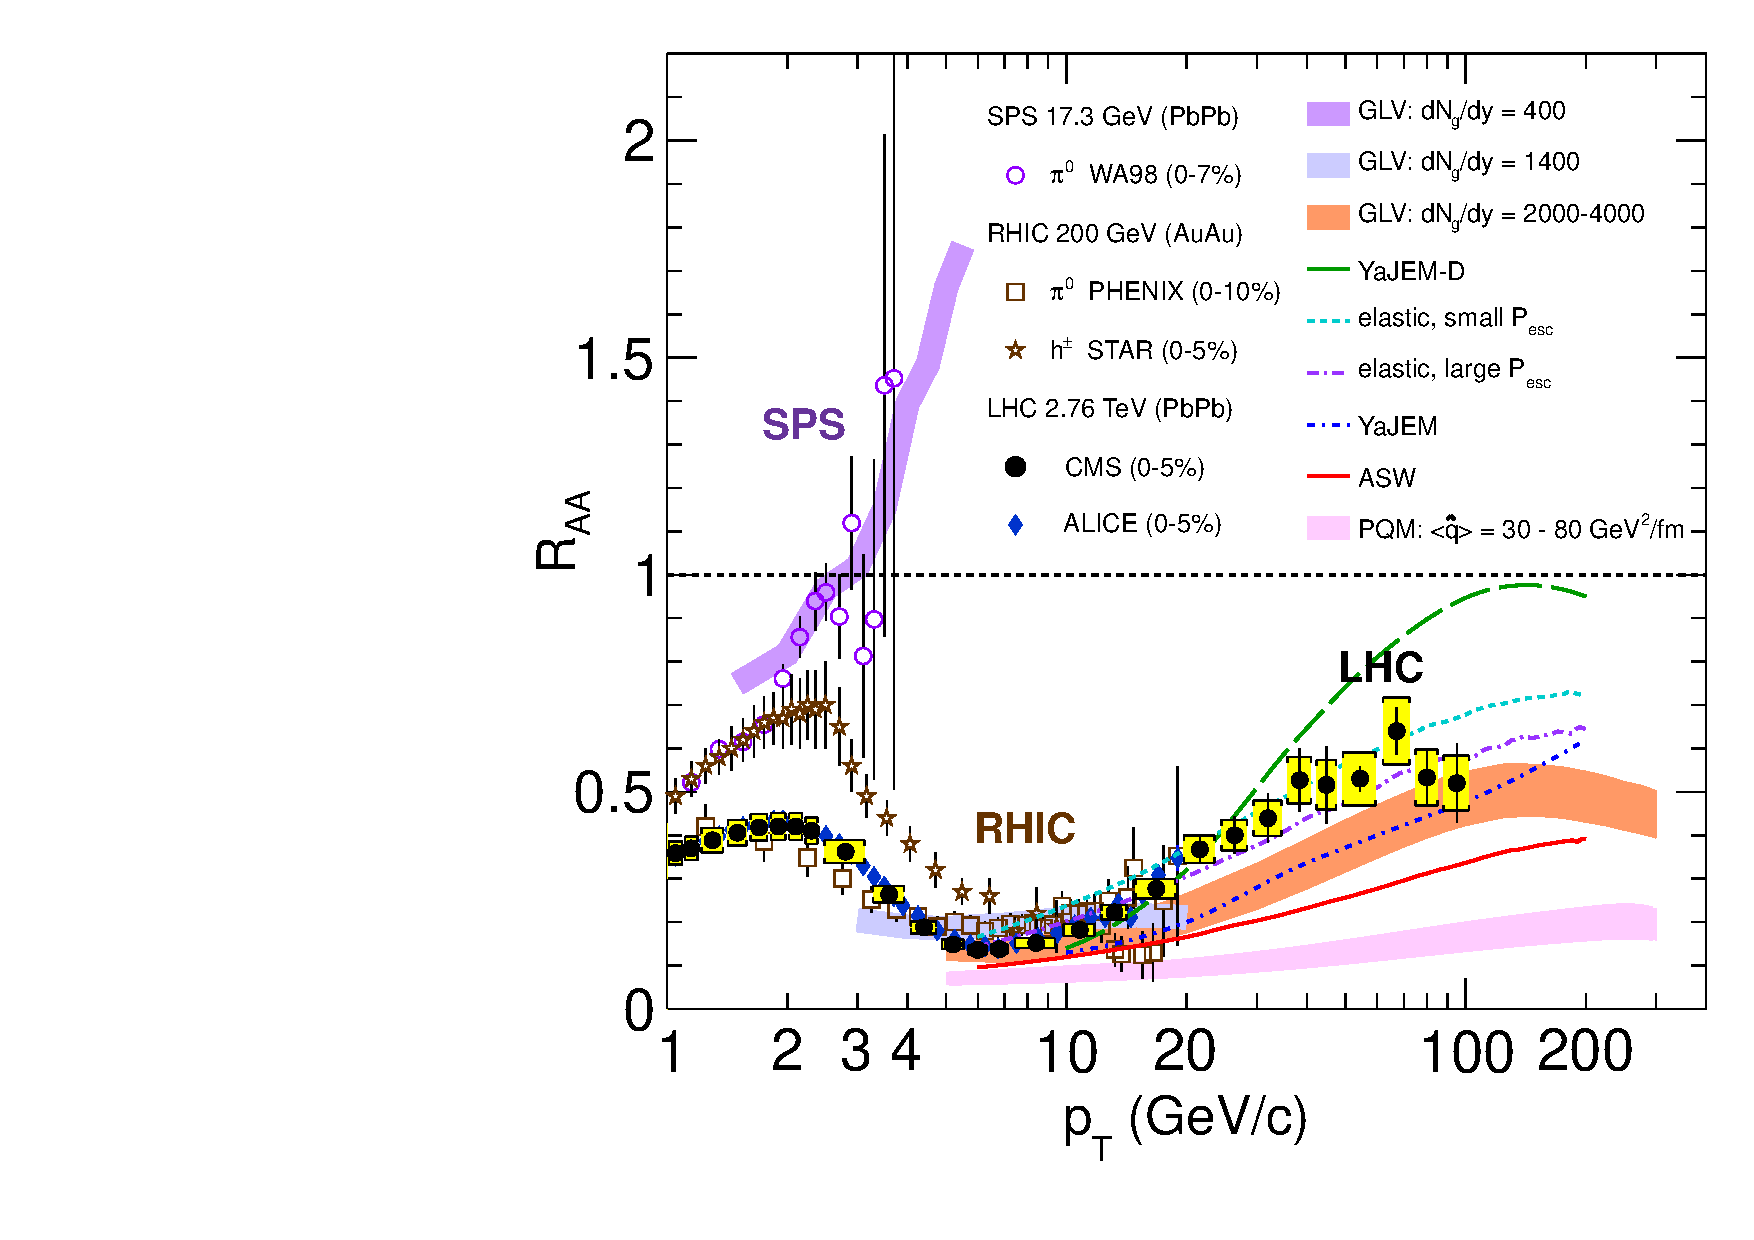
\includegraphics[width=0.5\textwidth]{particlefigs/CMSRAA.pdf}
\caption{Transverse momentum dependence of nuclear modification factor $R_{\rm AA}$ for charged particles produced in central heavy-ion collisions at LHC and lower energies. The curves and bands represent different model calculations. Reproduced from~\cite{CMS:2012aa}.}
\label{figks:CMSRAA}
\end{figure}

The CMS and ALICE experiments also measured the $R_{\rm AA}$ $p_{\rm T}$ dependence for different collision centralities~\cite{CMS:2012aa,Abelev:2012hxa}. The charged-particle production is, as expected, less and less suppressed as one moves from central to peripheral Pb--Pb collisons. The ATLAS collaboration reported similar results, presented as $R_{\rm CP}$ as a function of $p_{\rm T}$, where $R_{\rm CP}$ stands for a quantity analogue  to that defined in Eq.~\ref{eqks:RAA} using the normalized ratio of heavy-ion results at different centralities (the subscript CP indicates the central-to-peripheral ratio), commonly using the most peripheral class available for normalization.
%R_AA from CMS up to 100 GeV
\subsection{Identified-Hadron Spectra}
\label{subsecks:identspectra}
Study of the particle composition as a function of $p_{\rm T}$ reveals a mass hierarchy, interpreted as resulting from a common radial-velocity flow created during the expansion of the dense-matter fireball. Such a collective flow arises in strongly interacting matter in the presence of a pressure gradient. Having the same velocity, heavier particles (e.g. protons) will acquire a larger momentum than lighter mesons. This should be a large effect at low \pt\ and disappear progressively with increasing \pt\ (for $p_{\rm T}$ values significantly larger than particle masses).

\begin{figure}
\centering
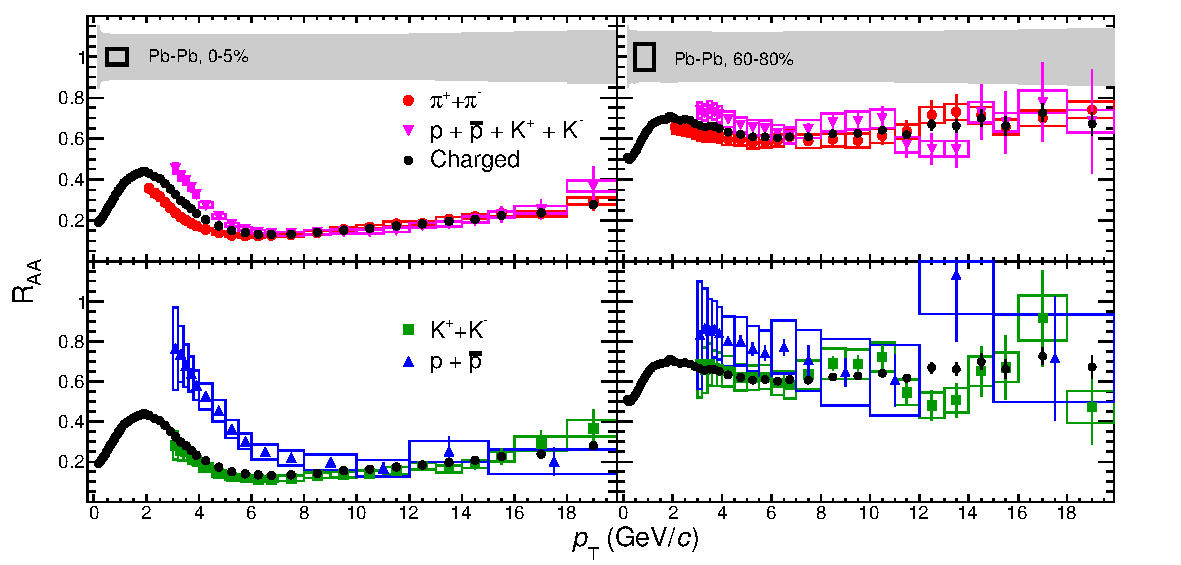
\includegraphics[width=0.7\textwidth]{particlefigs/IdentHighPtRAA.pdf}
\caption{Nuclear modification factor $R_{\rm AA}$ for pions, kaons, and protons (sum of particles and antiparticles), and averaged for charged particles, as a function of $p_{\rm T}$ for central (left, 0--5\,\%) and peripheral (right, 60--80\,\%) Pb--Pb collisions. Reproduced from~\cite{ALICEIdentHighPtRAA}.}
\label{figks:IdentPartRAA}
\end{figure}

The $p_{\rm T}$ spectra of identified charged hadrons are determined up to $p_{\rm T} = 20$~GeV~\cite{ALICEIdentHighPtRAA}. Figure~\ref{figks:IdentPartRAA} presents these results as $R_{\rm AA}$ for pions, kaons, and protons, compared to the (averaged) charged-particle data. It is clearly seen that for $p_{\rm T}$ above 7--8~GeV the behaviour for all particle species coincides. For lower $p_{\rm T}$ a mass hierarchy appears: the heavier the particle, the lower its suppression. A similar conclusion holds also for the strange particle production, such as $\Lambda$, $\Xi$, and $\Omega$~\cite{ABELEV:2013zaa,Abelev:2013xaa}. These observations suggest the existence of three regions in transverse momentum:
\begin{itemize}
    \item{bulk region, low $p_{\rm T}$ up to 2--3~GeV, where the production comes from the hadronization of high-density strongly-interacting matter created in a heavy-ion collision, reflecting collective radial flow, fairly described (at least for central collisions) by hydrodynamical models;}
    \item{intermediate region, in $p_{\rm T}$ up to 7--8~GeV, where still a mass splitting among various particle species persists that can be attributed a reminiscence of radial flow, however, additional ideas were put forward to push further in $p_{\rm T}$ this mass distinction, such as constituent-quark recombination which would favor baryons to acquire larger $p_{\rm T}$ than mesons;}
    \item{fragmentation region, above 7--8~GeV in $p_{\rm T}$, where the different hadron species exhibit a common suppression pattern, and consequently their relative abundances are the same as in pp collisions, naturally explained as being fragmentation products of a high-$p_{\rm T}$ parton coming from a hard scattering at early stage (which itself is quenched by the surrounding high-density matter).}
\end{itemize}

A detailed investigation of the intermediate region is performed by the measurement of the \pt\ dependence of the proton-to-pion~\cite{ALICEIdentHighPtRAA} and $\Lambda$-to-kaon~\cite{Abelev:2013xaa} ratios. For central collisions at $p_{\rm T}$ around 2.5--3~GeV these ratios are more than a factor three higher than the corresponding values for pp collisions. This so-called baryon anomaly was observed already at RHIC~\cite{Abelev:2006jr,Adare:2013esx}, and the low-$p_{\rm T}$ rise is well understood with the hydrodynamical radial flow. In the intermediate region, where the hydrodynamics ceases to work, the behavior is qualitatively described by models involving constituent-quark recombination~\cite{Fries:2003kq,Hwa:2006zq,Song:2007ux} or baryon string-junction transfer along the axis of a fragmenting jet~\cite{Aurenche:2011rd}. Recently, a good description has been obtained by EPOS model~\cite{Werner:2012xh}, where the interaction between bulk matter and jets is considered.
\subsection{High-\pt\ Particle Correlations}
\label{subsecks:correlation}
Two-particle correlations are used to study parton quenching at $p_{\rm T}$ below ${\cal O}(10)$~GeV~\cite{Aamodt:2011vg}, where the full jet reconstruction is difficult due to the underlying event fluctuations~\cite{Abelev:2012ej}. The correlation in the relative azimuthal angle $\Delta\varphi$ between a trigger particle within $8 < p_{\rm T}^{\rm t} < 15$~GeV and the associated particles with $p_{\rm T}^{\rm a}$ (a variable parameter), respecting $p_{\rm T}^{\rm a} <p_{\rm T}^{\rm t}$, has been studied~\cite{Aamodt:2011vg}. In order to measure the number of associated particles correlated to the trigger particle in the near-side and the away-side jet structures, the distribution after background subtraction is integrated around the near- and away-side peaks, in the $\pm 0.7$ and $\pi \pm 0.7$ $\Delta\varphi$ intervals, respectively. The per-trigger yields of associated particles, obtained this way, normalized to the same yields measured in pp collisions, represent the nuclear modification factor of the conditional yields, $I_{\rm AA}$. The near- and away-side $I_{\rm AA}$ are presented in Fig.~\ref{figks:IAA} as a function of associated-particle $p_{\rm T}^{\rm a}$. The results are practically independent on $p_{\rm T}^{\rm a}$, and for peripheral collisions compatible with no nuclear modification. For central collisions, the away-side $I_{\rm AA}$ is around 0.6, which is interpreted as a manifestation of jet quenching. On the near-side an enhancement for Pb--Pb with respect to pp collisions is observed, which could be understood a consequence of a modification of the fragmentation function, possibly caused by jet quenching and a trigger bias. This measurement constrains various models, some of those showed to be capable to describe such an effect~\cite{Renk:2011wp}.

\begin{figure}
\centering
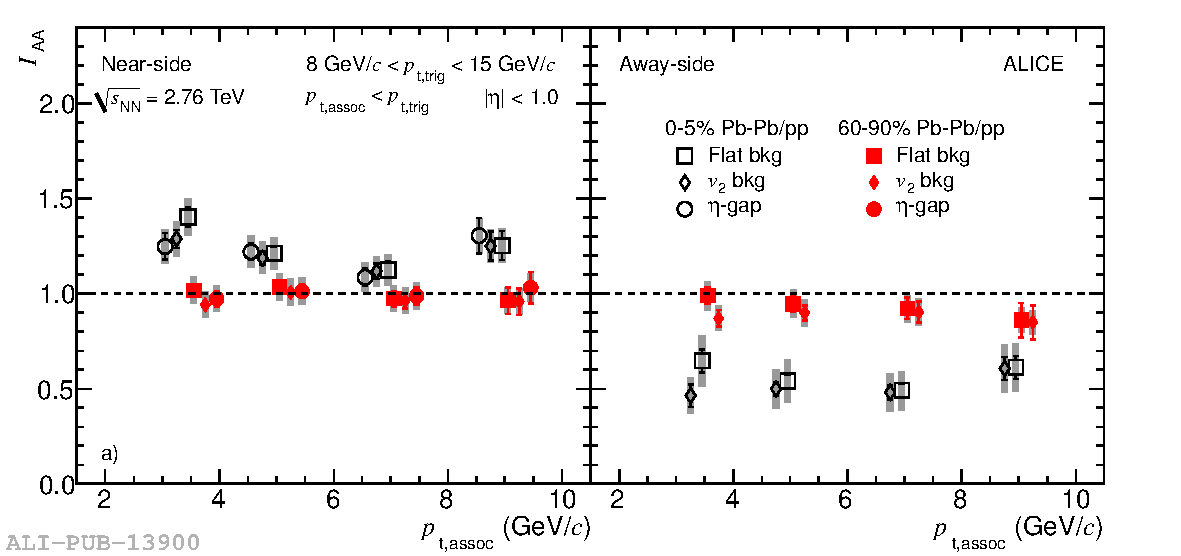
\includegraphics[width=0.7\textwidth]{particlefigs/IAA.pdf}
\caption{Near-side (left) and away-side (right) $I_{\rm AA}$ as a function of the transverse momentum of associated particles. The results are shown for peripheral (60--90\,\%) and central (0--5\,\%) Pb--Pb collisions. The three values shown for each measurement correspond to three background subtraction methods. Reproduced from~\cite{Aamodt:2011vg}.}
\label{figks:IAA}
\end{figure}

The triggered two-particle correlations in two dimensions, $\Delta\varphi$ and $\Delta\eta$ (pseudorapidity difference between trigger and associated particles), have been exploited to study the shape of the jet-structures~\cite{Morsch:2012gb}. The $\Delta\eta$ jet-structure width increases with the centrality of Pb--Pb collisions, while in the $\Delta\varphi$ direction such an increase, if any, is much reduced. This could be explained by a jet interaction with longitudinally flowing medium~\cite{Armesto:2004pt}. The particle composition of such jet-like structures is important for understanding of the in-medium modification of parton fragmentation. The proton-to-pion ratio has been measured in $(\Delta\varphi, \Delta\eta)$ regions, both inside and outside the jet structures selected in the correlation plot~\cite{Veldhoen:2012ge}. The jet p/$\pi$ ratio is obtained by correcting the jet-region value with properly weighted outside-jet (bulk) measurement. While the bulk p/$\pi$ ratio reproduces the baryon anomaly (see Sec.~\ref{subsecks:identspectra}), the jet ratio is compatible with the expectation for the jet fragmentation in pp collisions.


\section{HEAVY-FLAVOR PRODUCTION}
\label{heavyflavor}
Charm and beauty production provides a well calibrated probe for experimental investigation of heavy-ion collisions. The initial heavy-quark distributions are calculable from perturbative QCD and the calculations can be verified with pp measurements. However, the large advantage is that this probe is conserved from its production at early stage of the collision until it escapes from interaction region, and is eventually detected. This means that it is well tagged, which opens a possibility of a direct access to its interactions in the QGP, including the low- and intermediate-$p_{\rm T}$ regime. Two observables are usually studied: the nuclear modification factor $R_{\rm AA}$, and azimuthal-flow anisotropy, measured as the elliptic-flow coefficient $v_2$. They are closely connected: the in-medium heavy-quark energy loss decreases the momenta of heavy quarks, they may then thermalize in the surrounding matter, and thus participate in the evolution of collective-flow. The simultaneous measurement of the $R_{\rm AA}$ and $v_2$ enables the determination of the heavy-flavour transport coefficients.


Detection of heavy-flavor particles are done by two methods. The primary tool is invariant-mass reconstruction of exclusive particle decays in a secondary vertex, displaced from the interaction one. In the second method the heavy-flavor spectra are inferred from the lepton ($\mu^\pm$ or e$^\pm$) $p_{\rm T}$ spectra, presuming that these leptons are produced in semi-leptonic decays of heavy-flavor particles. However, this way a $p_{\rm T}$-dependent mixture of charm and beauty hadrons is measured. When possible, a requirement that the lepton is not coming from the interaction vertex is utilized, which significantly suppresses the background, especially at lower $p_{\rm T}$ (below 4~GeV). The B-meson production is also accessible with the inclusive decays ${\rm B} \rightarrow {\rm J}/\psi + X$, demanding the J/$\psi$ decay vertex to be separated from the interaction point.

\subsection{Heavy-Flavor Spectra}
\label{subsecks:heavyspectra}
The $p_{\rm T}$ spectra of heavy-flavour particles are measured by ALICE in pp and Pb--Pb (and p--Pb) collisions. The pp results are compared to perturbative QCD calculations and other models~\cite{ALICE:2011aa,Abelev:2012vra}, giving information about preferred values for parameters, such as renormalization and factorization scales. The charm-particle spectra are measured down to very low $p_{\rm T}$ (about 1~GeV in pp) allowing for precise determination of the total charm cross section at LHC energies. The pp spectra also serve as a normalization for Pb--Pb measurements~\cite{ALICE:2012ab}.

The heavy-flavor spectra in heavy-ion collisions are expected to be also suppressed with respect to those in pp interactions, due to the energy quenching of heavy quark when traversing the dense medium. However, the energy loss of heavy quarks is predicted to be different than that of light quarks and gluons. The energy loss of quarks by bremsstrahlung radiation will be quark-mass dependent. Due to a destructive interference, such gluon radiation is suppressed in directions close to that of the initial quark, for angles smaller than $\Theta_0 \approx m/E = 1/\gamma$ ($m$, $E$, and $\gamma$ being the quark mass, energy, and gamma-factor, respectively). At a fixed momentum, this exclusion region (i.e. $\Theta_0$) is larger for the heavier quarks, resulting in smaller energy loss for heavy quarks compared to that for the light ones. This is the so called dead-cone effect originally described for the QCD radiation in vacuum~\cite{Dokshitzer:1991fc}, and later applied to the medium-induced radiation in a similar manner~\cite{Dokshitzer:2001zm}. The predicted mass hierarchy is stronger at $p_{\rm T}$ comparable with quark masses, and diminished progressively at very high $p_{\rm T}$. Recent model calculations include both the radiation and collisional energy losses, which increases the suppression of heavy quarks, and results in \Raa\ values closer to the expectation for light quarks.

Other effects that can modify the expected suppression pattern have to be taken into account. Contrary to heavy-flavor hadrons produced by fragmentation of the corresponding heavy quarks, the light-flavor particles at $p_{\rm T} \sim {\cal O}(10)$~GeV are, at the LHC energies, mostly produced in gluon fragmentation. However, gluons have by a factor 9/4 larger color charge than quarks, and consequently a gluon is loosing more energy than a quark. This color-charge effect is enlarging the expected difference in suppression between the light- and heavy-flavor particles. Another effects of less importance are taken into account in various models, such as nuclear modification of structure functions and harder fragmentation function of heavy quarks compared to the light sector.

Charm mesons are identified reconstructing the following decays: ${\rm D}^0 \rightarrow {\rm K}^-\pi^+$, ${\rm D}^+ \rightarrow {\rm K}^-\pi^+\pi^+$, and ${\rm D}^{*+} \rightarrow {\rm D}^0\pi^+$ (and their antiparticles), requiring the decay vertex to be displaced from the interaction point. The D-meson yields are corrected for the feed-down from beauty decays, based on model simulations. The B-decay contribution amounts to 5--15\,\% of the yields, depending on $p_{\rm T}$ and the particle type. The nuclear modification factor $R_{\rm AA}$ is calculated from the measured $p_{\rm T}$ spectra for both pp~\cite{ALICE:2011aa,Abelev:2012vra} and Pb--Pb~\cite{ALICE:2012ab} collisions. 

 As expected, the \Raa\ $p_{\rm T}$ dependencies for three D-mesons are compatible. Therefore, an average D-meson $R_{\rm AA}$ is calculated combining the results according their statistics, dominated by the ${\rm D}^0$. The average D-meson $R_{\rm AA}$ in central Pb--Pb collisions as a function of $p_{\rm T}$ is compared with that of charged particles in Fig.~\ref{figks:DmesonRAA}. The D-meson $R_{\rm AA}$ might be slightly above the charged-particle one, hinting at less charm-quark suppression, but the difference, if any, is very small. This tendency was recently confirmed with higher statistics charm measurements. The model calculations overlayed on data in Fig.~\ref{figks:DmesonRAA} are (I)~\cite{Sharma:2009hn,He:2011pd}, (II)~\cite{Horowitz:2011cv}, (III)~\cite{Horowitz:2011wm}, (IV)~\cite{Alberico:2011zy,Monteno:2011gq}, (V)~\cite{Gossiaux:2009mk,Gossiaux:2010yx}, (VI)~\cite{Fochler:2011en}, (VII)~\cite{Buzzatti:2011vt}, and (VIII)~\cite{Armesto:2005iq}. Varying degrees of agreement with the charm results are shown by various models. In general the inclusion of collisional energy loss improves the model description. In model (I) the larger D suppression is obtained by introducing in-medium dissociation of D mesons, in addition to radiative energy loss. The remaining models that compute also the charge-particle $R_{\rm AA}$, have not reached good description for both cases, albeit some being not far.

\begin{figure}
\centering
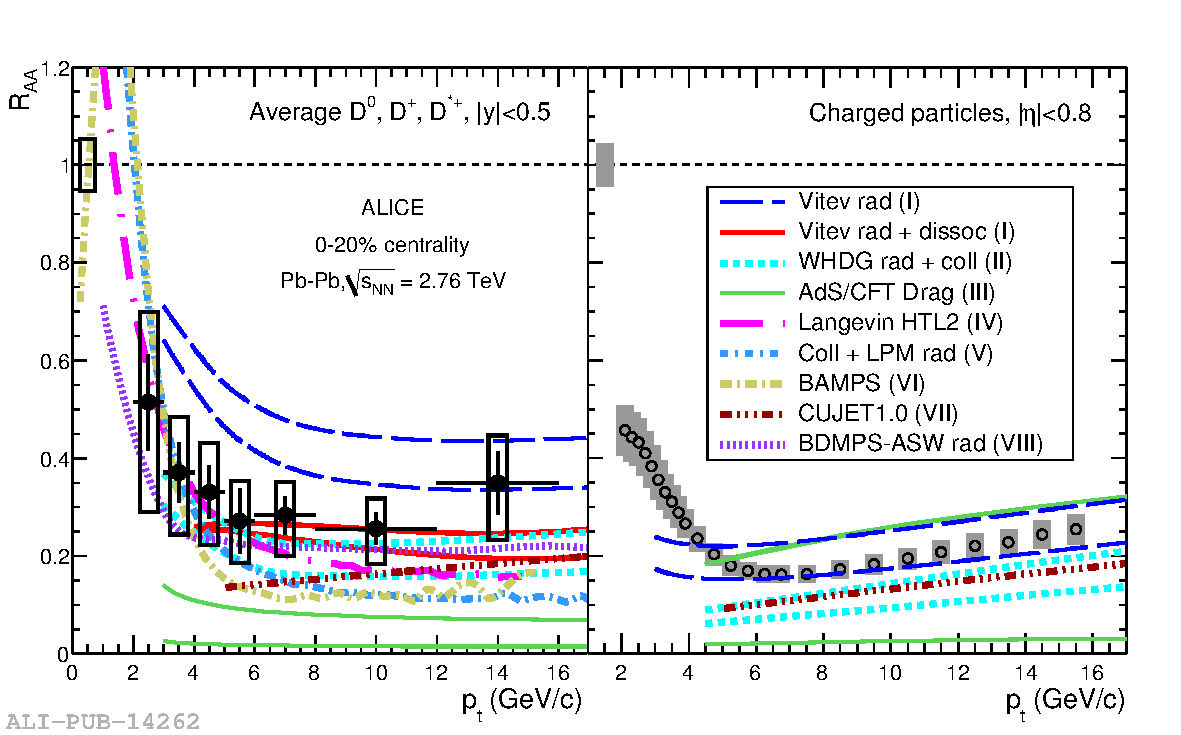
\includegraphics[width=0.7\textwidth]{heavyflavorfigs/DmesonChargedRAAmodels.pdf}
\caption{Average D-meson $R_{\rm AA}$ (left) and charged particle $R_{\rm AA}$ (right) as a function of $p_{\rm T}$ for the centrality between 0--20\,\%. The normalization uncertainties shown at unity in abscissa are almost fully correlated. The curves represent various model calculations, referred in the text, some of them are shown as a range. Reproduced from~\cite{ALICE:2012ab}.}
\label{figks:DmesonRAA}
\end{figure}

The family of measured D mesons was enlarged recently with the study of ${\rm D}_{\rm s}^+ \rightarrow {\rm K}^+{\rm K}^-\pi^+$ decay~\cite{Abelev:2012tca}. The presence of strange quark may lead to a relative increase of ${\rm D}_{\rm s}$ production with respect to other D-mesons, as a consequence of general strangeness enhancement observed in heavy-ion collisions. Preliminary results show the ${\rm D}_{\rm s}$ $R_{\rm AA}$ in $p_{\rm T}$ region 4--12~GeV above the D-meson $R_{\rm AA}$, however, still within large uncertainties.

The behavior of the charm-meson $R_{\rm AA}$ has been confirmed by the ALICE measurement of the muon spectrum in the forward region $2.5 < y < 4$~\cite{Abelev:2012qh}. The estimated pion- and kaon-decay contribution is subtracted from the measured muon spectrum, this contamination falls below 10\,\% for $p_{\rm T} > 4$~GeV, where the results are presented. The corrected muon $p_{\rm T}$ spectrum thus represents the result for a mixture of muons from semi-leptonic charm and beauty decays, presumably charm dominated at $p_{\rm T}$ about 4~GeV and progressively becoming beauty dominated for $p_{\rm T} > 6$~GeV. The heavy-flavor muon $R_{\rm AA}$, using an analogous analysis of pp data for normalization, is presented in Fig.~\ref{figks:HFmuonRAA}. The muon $p_{\rm T}$, being correlated with the heavy-flavor-particle $p_{\rm T}$, is systematically smaller than the latter one (for $p_{\rm T}$ above a few GeV). The comparison with the D-meson $R_{\rm AA}$ shows qualitative agreement, since the $p_{\rm T}$ dependence is rather flat. A similar measurement exploiting electron detection in mid-rapidity region has been also reported~\cite{Abelev:2012xe}.

\begin{figure}
\centering
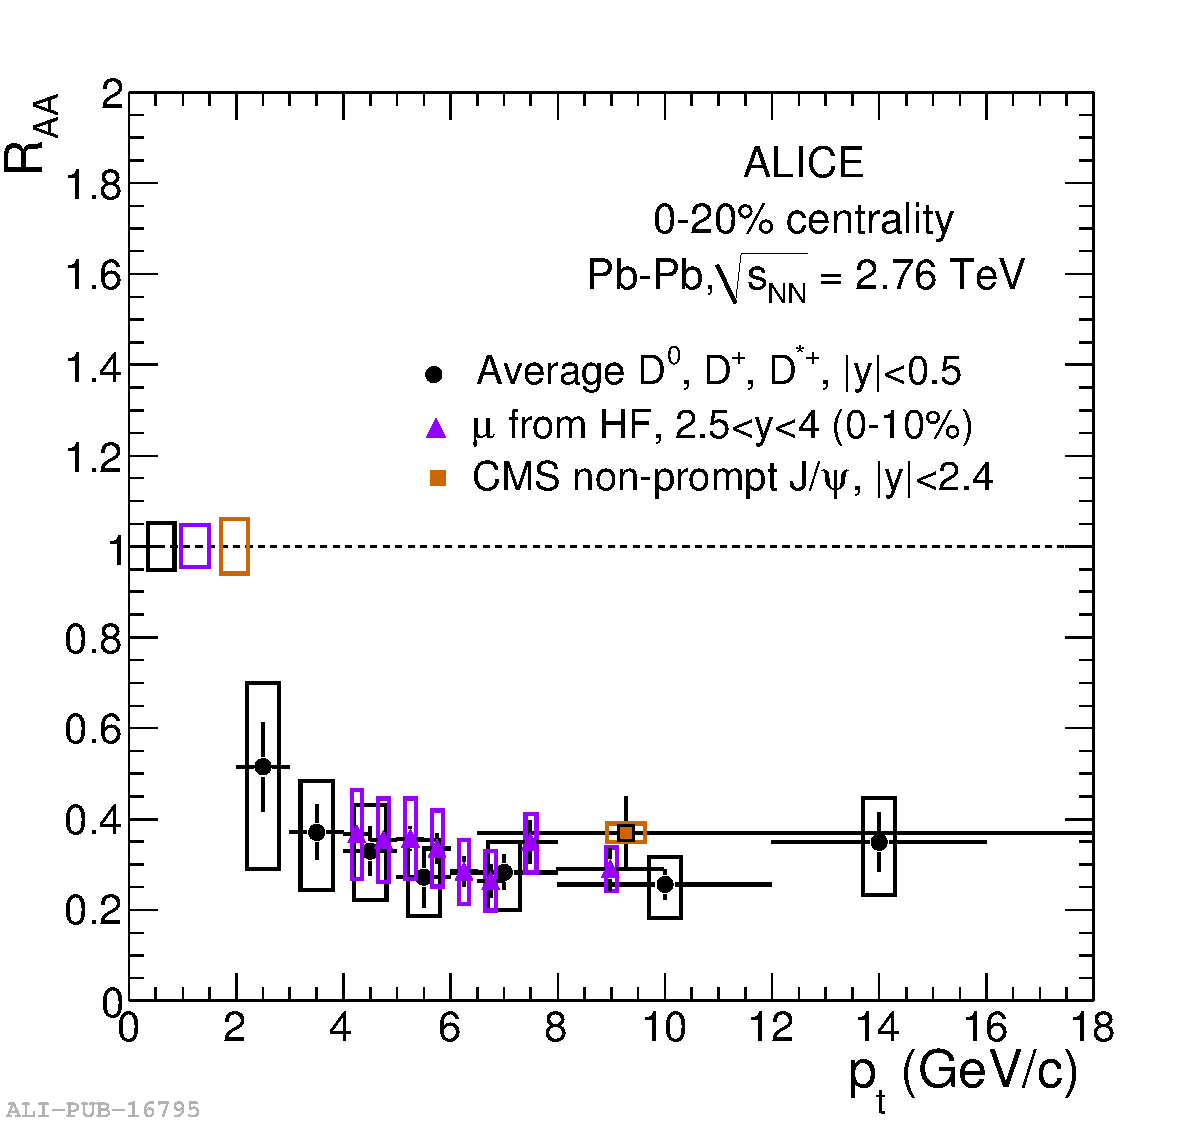
\includegraphics[width=0.5\textwidth]{heavyflavorfigs/DmesonHFmuonBRAA.pdf}
\caption{Heavy-flavor muon $R_{\rm AA}$ as a function of $p_{\rm T}$ compared to the average D-meson $R_{\rm AA}$. Results are for 0--20\,\% centrality class of Pb--Pb collisions. CMS preliminary result for beauty $R_{\rm AA}$ from measurement of non-prompt J/$\psi$ is shown with square. Reproduced from~\cite{Abelev:2012qh}.}
\label{figks:HFmuonRAA}
\end{figure}

The preliminary CMS result for $R_{\rm AA}$ from the measurement of non-prompt J/$\psi$ is also shown~\cite{Chatrchyan:2012np} in Fig.~\ref{figks:HFmuonRAA}. The position of the J/$\psi$-decay point with respect to interaction vertex is used to select the non-prompt J/$\psi$ particles, they are practically exclusively coming from B-meson decays. Higher-statistics results on the centrality dependence of the $R_{\rm AA}$ for non-prompt J/$\psi$~\cite{CMS:2012wba} (in $p_{\rm T}$ range 6.5--30~GeV) compared to the ALICE D-meson data (in $p_{\rm T}$ range 8--16~GeV) demonstrate the smaller suppression for the beauty production than for the charm production, except for peripheral collisions, where the measurements are within their uncertainties. The difference between the $p_{\rm T}$ ranges takes into account that the J/$\psi$ momentum is lowered in the decay. For the first time the predicted hierarchy of the charm and beauty energy loss is experimentally confirmed.

\subsection{Charm Elliptic Flow}
\label{subsecks:heavyflow}
The elliptic azimuthal asymmetry is caused by the asymmetric collision geometry: in semi-central collisions the overlapping region of the two colliding nuclei has an almond shape, elongated in the direction perpendicular to the event plane (the plane defined by the beam axis and the centres of the two nuclei). This initial space asymmetry is transferred by the pressure created in the medium into the asymmetry in the azimuthal momentum distribution, resulting in more final particles produced in the event plane than out of the event plane. The azimuthal distribution is described by $\propto 1 + v_2 \cos{2(\varphi - \psi)}$, where $\varphi - \psi$ is the particle azimuthal angle with respect to the event-plane at azimuthal angle $\psi$, and the coefficient $v_2$ characterizes the amplitude of the azimuthal modulation. The position of the event plane $\psi$ is estimated with a set of the particle tracks in the same event.

The elliptic flow of charm has been studied by ALICE for the three mesons: ${\rm D}^0$, ${\rm D}^+$, and ${\rm D}^{*+}$, and, as the $v_2$ values are compatible, they are then averaged applying beforehand the feed-down correction like in the case of the D-meson $R_{\rm AA}$. The $v_2$ results for the average D meson are presented in Fig.~\ref{figks:DmesonV2} for the centrality in the range 30--50\,\%. The comparison with the charged-particle $v_2$ obtained with the same method reveals that the $v_2$ values for $p_{\rm T}$ between 2--8~GeV are compatible. This is the first direct observation of non-zero $v_2$ for a heavy-flavor particle. The large value of the charm $v_2$ at $p_{\rm T}$ around 2~GeV is interpreted as a signature of the in-medium thermalization of charm quarks. The challenge now is a simultaneous model description of the charm \Raa\ and $v_2$ measurements. This needs a detailed transport model calculations as the results are sensitive to the time evolution of the suppression and the elliptic-flow build-up.

\begin{figure}
\centering
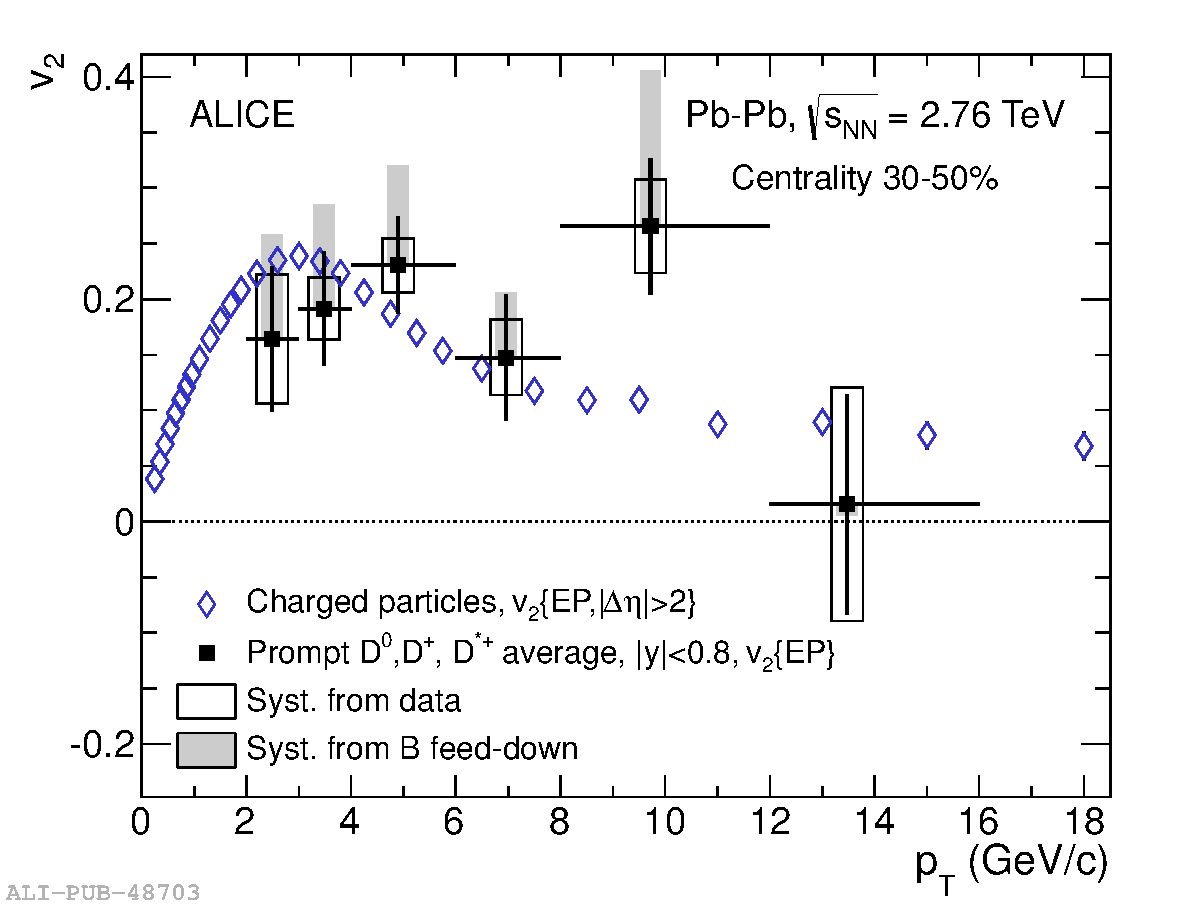
\includegraphics[width=0.5\textwidth]{heavyflavorfigs/DmesonV2.pdf}
\caption{Elliptic-flow coefficient $v_2$ obtained with the event-plane method, as a function of $p_{\rm T}$ for the centrality 30--50\,\%, averaged for ${\rm D}^0$, ${\rm D}^+$, and ${\rm D}^{*+}$, compared to the charged-particle measurement. Reproduced from~\cite{Abelev:2013lca}.}
\label{figks:DmesonV2}
\end{figure}

At higher $p_{\rm T}$ a positive $v_2$ can be generated by the difference in the in-medium path lengths for charm quarks emitted in-plane compared to those emitted in out-of-plane. The shorter path length for the in-plane partons implies less suppression, i.e. larger $R_{\rm AA}$ for particles produced in this direction, than for those produced in the out-of-plane direction. In fact, the results can be presented as an azimuthally-dependent $R_{\rm AA}$, which is equivalent to the azimuthally-integrated $R_{\rm AA}$ and the $v_2$. The interpretation of the high-$p_{\rm T}$ $v_2$ as a path-length effect opens the possibility of studying  the in-medium path-length dependence of the parton energy loss.

The $v_2$ results for D mesons are complemented by the recently reported elliptic-flow measurements at forward rapidities ($2.5 < y < 4$) for the muons from heavy-flavour decays. They show an effect of similar magnitude. Indication of non-zero heavy-flavour $v_2$ using the semi-leptonic decays were previously published by RHIC experiments~\cite{Adler:2005ab,Adare:2006nq}. 

\section{QUARKONIA}
\label{quarkonia}
Quarkonium production is believed to give important information about the
hot and dense matter formed in heavy-ion collisions.
The in-medium suppression  of quarkonium states caused by Debye screening of the color potential between heavy quarks
is expected to depend on the their binding energy and the temperature of the medium, leading to a sequential
disappearance of the various charmonium and
bottomonium states~as the temperature increases\cite{Matsui:1986dk,Digal:2001ue,Mocsy:2007jz}. Therefore, the measurement of the quarkonium suppression pattern is sometimes called the QGP thermometer. At the increase of the temperature, first the higher-mass (less bound) states, such as \psip\ and \PgUc\, are melted, then \Jpsi\ and \PgUb\ at approximately the same point, and finally the most tightly bound \PgUa\ is expected to disappear only at very high temperature (about twice the critical temperature). However, a significant fraction of the lower-mass states is normally produced as a decay product of the higher-mass states, including those difficult to observed directly, e.g. \chic\ and $\chi_{\rm b}$, therefore \Jpsi\ and \PgUa\ can be suppressed even if their corresponding melting temperatures are not reached.

Suppression of \Jpsi\ production was clearly observed in central heavy-ion collisions at CERN SPS~\cite{Baglin:1994ui,Alessandro:2004ap,Alessandro:2006ju,Arnaldi:2007zz}, and an effect on about the same level was later measured at RHIC~\cite{Adare:2006ns,Adare:2011yf}. The quantitative interpretation of the observed suppression is complicated by cold nuclear-matter effects, such as the modification of nuclear structure functions and final state absorption. At higher collision energies, when the production of charm becomes more abundant, the charmonium states can be regenerated~\cite{BraunMunzinger:2000px,Thews:2000rj,Andronic:2007bi,Zhao:2007hh,Capella:2007jv}. At the LHC in a central Pb--Pb collision ${\cal O}(100)$ c$\overline{\rm c}$ pairs are produced, and they may recombine during the hadronization into charmonia, thus compensating the initial suppression. The regeneration yield is strongly dependent on  the c$\overline{\rm c}$ quark density, and therefore can be inferred from the measurement in different kinematical regions and at different collision energies. At the LHC energies the feed-down of charmonium states from B-hadron decays is sizeable. This can be exploited for B-production measurements, as explained in Sec.~\ref{subsecks:heavyspectra}, and data for charmonium production are presented corrected for such feed-down, i.e prompt J/$\psi$, or without this correction, i.e. inclusive J/$\psi$.

The large advantage brought by the LHC energy is the increase of the quarkonium cross sections, and this is especially beneficial for $\Upsilon$ family allowing for high statistics measurement for the first time. The three observed $\Upsilon$ states have very similar initial conditions, therefore the expected suppression pattern reflects the hierarchy of their binding energies, with possible (small) absorption corrections. The regeneration effect in this case will be negligible, due to order of magnitude lower b-quark density compared to that of c quarks.

\subsection{Charmonium Production}

The ATLAS and CMS experiments are measuring \Jpsi\ production in the dimuon channel for relatively high $p_{\rm T}$~\cite{Aad:2010aa,Chatrchyan:2012np}, above 3--6.5~GeV, depending on the rapidity range. ALICE is capable to detect charmonia down to zero \pT\ both in the dimuon channel in forward region ($2.5 < y < 4$)~\cite{Abelev:2012rv}, and in the dielectron channel in the mid-rapidity region ($|y| < 0.9$)~\cite{Abelev:2013ila}. The results are usually presented in terms of the nuclear modification factor, $R_{\rm AA}$, defined in Eq.~\ref{eqks:RAA}.

The rapidity dependence of the inclusive \Jpsi\ $R_{\rm AA}$, integrated over centrality and $p_{\rm T} > 0$ (or $> 3$~GeV)~\cite{Abelev:2012rv,Abelev:2013ila}, does not show a strong variation up to $y = 3$ and the $R_{\rm AA}$ is around 0.7 for $p_{\rm T} > 0$. At higher rapidities, up to $y = 4$, there is a tendency for more suppression, the $R_{\rm AA}$ value decreases down to 0.4. At higher \pT\ ($> 6.5$~GeV), the \Jpsi\ suppression is stronger, and was measured separately for prompt and non-prompt \Jpsi~\cite{Chatrchyan:2012np,CMS:2012wba}, with the centrality and \pT\ integrated \Raa\ found to be about 20\,\% lower for prompt than for non-prompt \Jpsi.

\begin{figure}[!ht]
\begin{center}
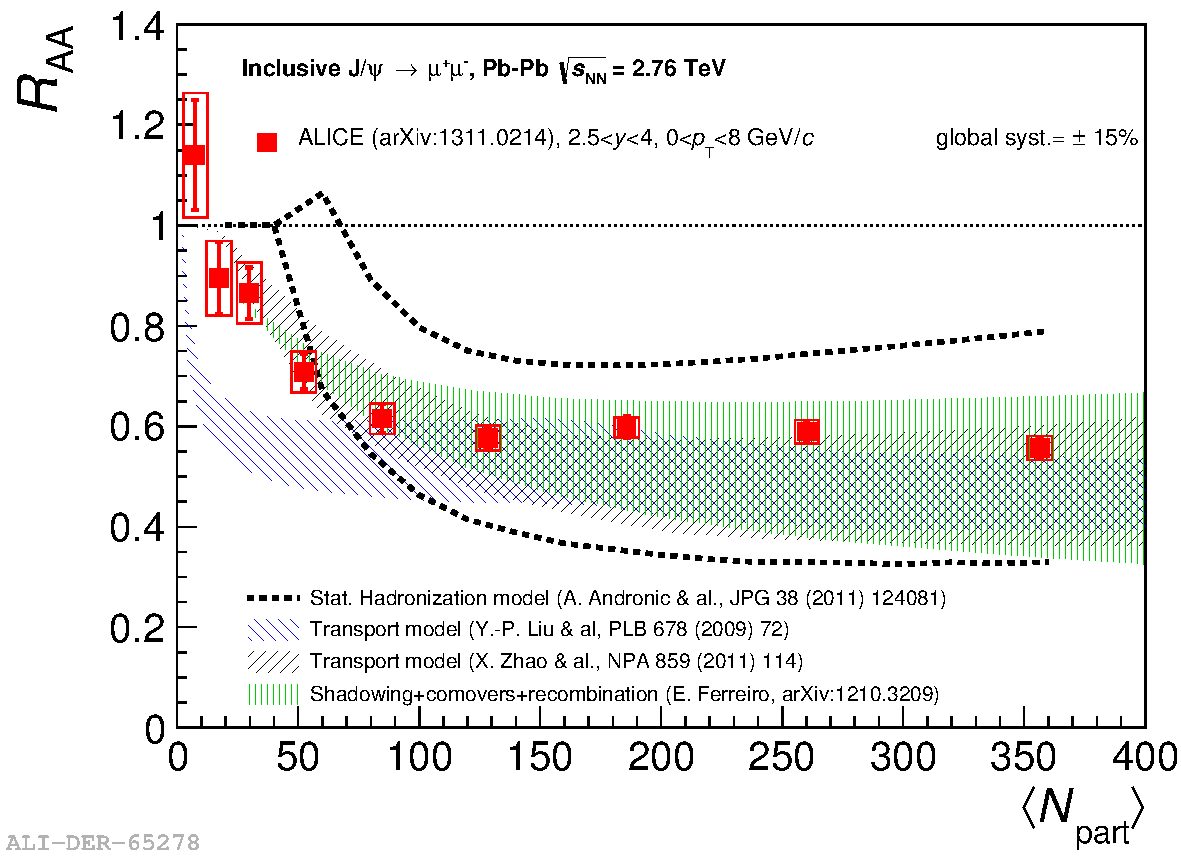
\includegraphics[width=0.49\linewidth]{quarkoniafigs/JpsiRAAcentrality.pdf}
\label{fig:KS:RaavsCent} 
\caption{Inclusive \jpsi\ \Raa\ measured in \PbPb\
collisions at $\rootsNN = 2.76$\TeV\ as a function of $N_{part}$ for two \pT\ ranges.
Total systematic uncertainties are displayed as open boxes.The experimental measurements are compared with
model calculations~\cite{Andronic:2011yq,Liu:2009nb,Zhao:2011cv,Ferreiro:2012rq}, which all include \Jpsi\ regeneration effects. Figure adapted from~\cite{Abelev:2012rv}.}
\end{center}
\end{figure}

In the forward rapidity region ($2.5 < y < 4$) detailed measurements of the \Jpsi\ \Raa\ were performed by ALICE. The centrality dependence, expressed as a function of $N_{\rm part}$, is presented in Fig.~\ref{fig:KS:RaavsCent} for $\pt > 0$. For $N_{\rm part} > 100$ (corresponding to about 40\,\% most central collisions) the inclusive \Jpsi\ suppression is approximately constant, with \Raa\ about 0.5--0.6. Moving to more peripheral collisions, the nuclear modification factor increases progressively eventually becoming consistent with unity. This centrality behavior is qualitatively different compared to that measured in forward region by PHENIX~\cite{Adare:2011yf}. At RHIC the \Jpsi\ nuclear modification factor steadily decreases with increasing $N_{\rm part}$, falling to 0.2 for most central collisions, which means almost three times stronger \Jpsi\ suppression compared to central LHC collisions.

CMS measured the centrality evolution of the \Jpsi\ suppression at $\pt > 6.5$~GeV and at mid-rapidity $|y| < 2.4$~\cite{Chatrchyan:2012np,CMS:2012wba}; the result for the prompt \Jpsi\ \Raa\ at this higher \pt\ resemble the (low-\pt) RHIC observation. Even though the non-prompt (B-decay) \Jpsi\ are less suppressed than the prompt ones, and hence the feed-down correction would decrease the inclusive \Raa\ values, this will not qualitatively affect the conclusion about the difference between RHIC and the LHC. This correction for the relevant centralities and \pt, estimated using the difference between the non-prompt and prompt \Raa\ and the measured fraction of B-decay \Jpsi\ at the LHC~\cite{Khachatryan:2010yr,Aaij:2011jh,Aad:2011sp,Chatrchyan:2012np,Abelev:2012gx}, is below 10\,\%, and only a few percents at lower \pt.

The observed suppression is stronger than that predicted for shadowing effects in the Color Singlet
Model~\cite{Ferreiro:2011rw} and the Color Evaporation Model~\cite{Vogt:2010aa}. Neither of these models predicts a strong rapidity dependence. A stronger initial-state suppression has been calculated in the Color Glass Condensate
(CGC) model~\cite{Dominguez:2011cy}, predicting  \jpsi\ \Raa\ about 0.5. However, important information is provided by the \pT\ dependence of \Jpsi\ suppression. Initial state suppression models typically lead
to a stronger suppression at lower \pT. Contrary to this, \Jpsi\ regeneration effects in statistical-hadronization~\cite{BraunMunzinger:2000px,Thews:2000rj} and in partonic-transport~\cite{{Zhao:2007hh},{Liu:2009nb}} models are expected to enhance \Jpsi\ yields at low \pT\ due to the higher phase-space density of charm quarks there. The calculations obtained with models including \Jpsi\ regeneration are compared to the (low-\pt dominated) \Jpsi\ \Raa\ measurement in Fig.~\ref{fig:KS:RaavsCent}, and they overall describe data rather well, especially for semi-peripheral to central collisions.

\begin{figure}[!ht]
\begin{center}
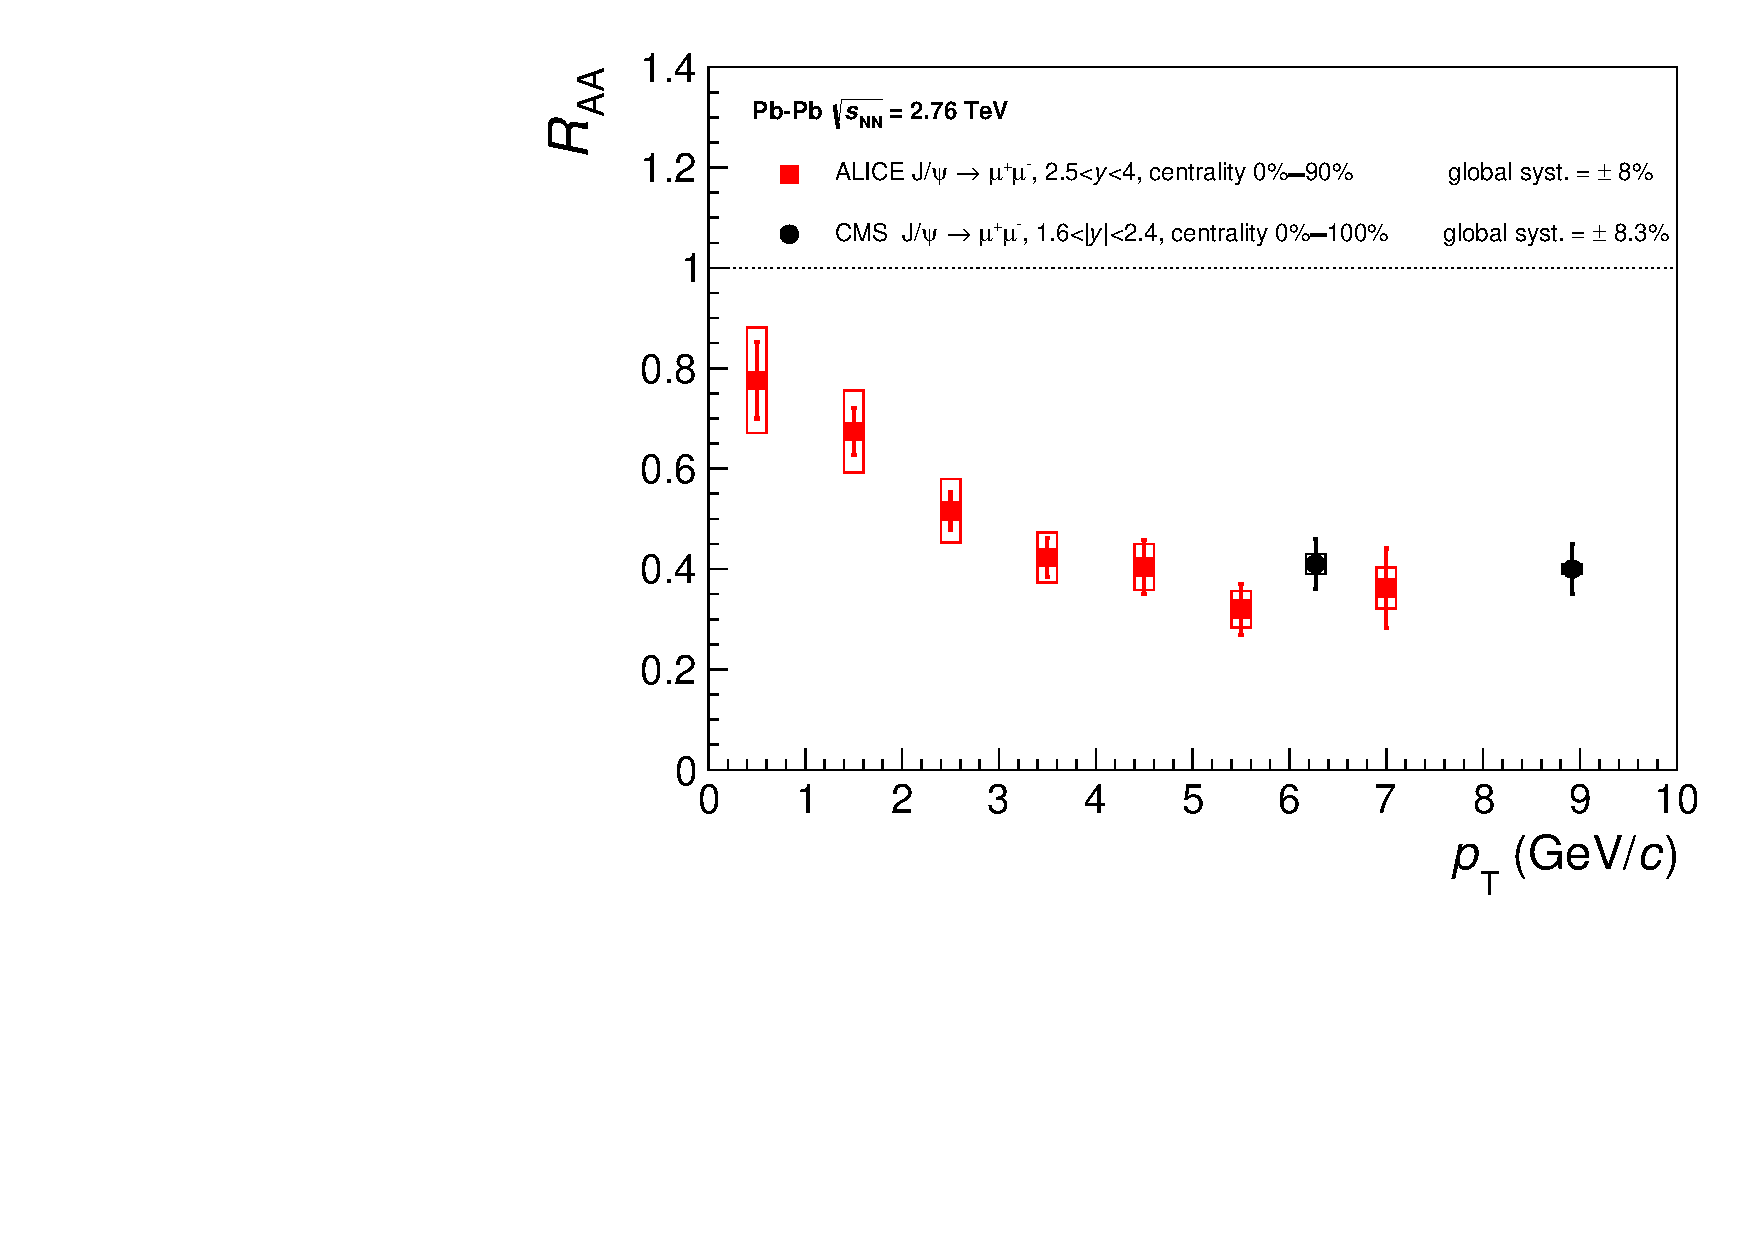
\includegraphics[width=0.49\linewidth,keepaspectratio]{quarkoniafigs/RAAPtvsModels1.pdf}
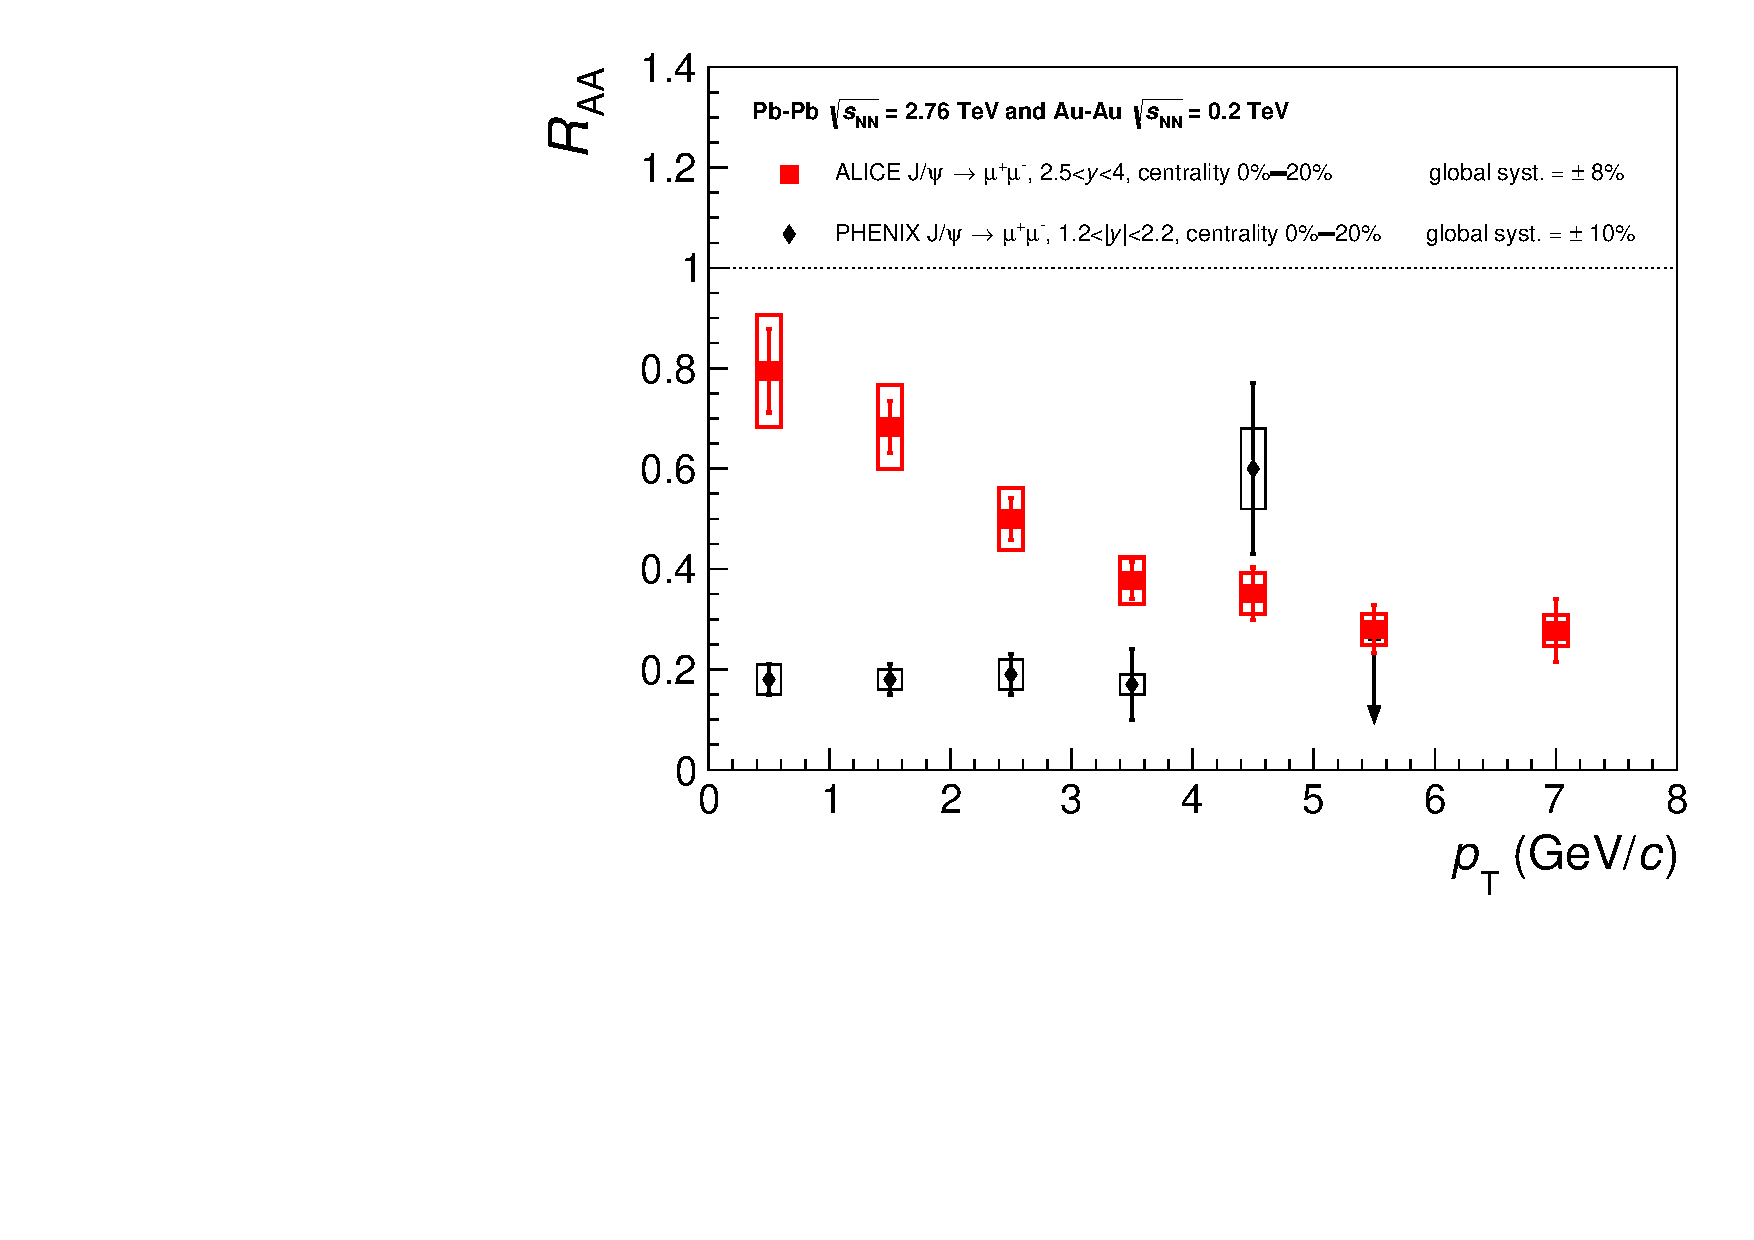
\includegraphics[width=0.49\linewidth,keepaspectratio]{quarkoniafigs/RAAPtvsModels2.pdf}
\caption{ \label{fig:KS:RaaPt}
(Left): Transverse momentum dependence of \Jpsi\ \Raa\ measured by ALICE~\cite{Abelev:2013ila} (0--90\,\% centrality) and by CMS~\cite{Chatrchyan:2012np} (0--100\% centrality) in \PbPb\
collisions at $\rootsNN = 2.76$\TeV.
(Right): Transverse momentum dependence of the \Jpsi\ \Raa\ measured by ALICE in the 0\%--20\% most
central \PbPb\ collisions at 2.76\TeV\ compared to PHENIX~\cite{Adare:2011yf}
results in the 0\%--20\% most central \AuAu\ collisions at 200\GeV. Reproduced from~\cite{Abelev:2013ila}}
\end{center}
\end{figure}

In Fig.~\ref{fig:KS:RaaPt} the inclusive \Jpsi\ $R_{\rm AA}$ dependence on transverse momentum is presented: (left) integrated over centrality, and (right) for the top 20\,\% of central collisions, compared to the PHENIX result. In both centrality ranges at the LHC the \Jpsi\ is little suppressed at low \pt\ ($\Raa \approx 0.8$ at \pt\ 0--1~GeV) and much more strongly suppressed at $\pt > 5$~GeV ($\Raa \approx 0.4$ for centrality integrated data, $\Raa \approx 0.25$ for 20\,\% of most central collisions). The comparison to the \pt\ dependence measured at RHIC, where the \Jpsi\ is strongly suppressed already at low \pt\ and no further decrease od \Raa\ is observed with increasing \pt, confirms the new regime of \Jpsi\ production achieved at the LHC. These results are qualitatively consistent
with the expectations of recombination approaches such as~\cite{Zhao:2007hh,Zhou:2013aea,Liu:2009nb}, while a quantitative interpretation of this result will require
a detailed understanding of cold-nuclear-matter effects. First results on \Jpsi\ production in \pPb\ collisions at the LHC have recently been published~\cite{Abelev:2013yxa,Aaij:2013zxa}, allowing the direct measurement of such effects.

\subsection{Charmonium Elliptic Flow}

For the study of the \Jpsi\ production mechanism, in addition to the $R_{\rm AA}$, the precise measurement of the elliptic flow is an important ingredient. Like for open charm production (Sec.~\ref{subsecks:heavyflow}) the value of the elliptic-flow parameter $v_2$ reflects the degree of thermalization of charm quarks. If charm quarks participate in the collective expansion of the medium, as suggested by the observed elliptic flow of open charm mesons, \jpsi\ produced by recombination should acquire the elliptic flow of these charm quarks.

At RHIC the \Jpsi\ elliptic flow was measured by the STAR collaboration~~\cite{Adamczyk:2012pw}. The $v_2$ for Au--Au collisions at highest RHIC energy $\rootsNN = 200$~GeV is compatible with zero, however, with rather large uncertainties, which do not allow a definite conclusion. At the LHC, ALICE has reported a non-zero \Jpsi\ $v_2$ with a significance of 2.1 standard deviations~\cite{ALICE:2013xna}. This result is presented in Fig.~\ref{fig:KS:v2ptcomp} as the transverse-momentum dependence of the \Jpsi\ $v_2$ for Pb--Pb collisions at $\rootsNN = 2.76$~TeV in the centrality range 20--60\,\%, i.e. semi-central collisions, where a maximal effect is expected. The measurements are compared with two model calculations~\cite{Liu:2009gx,Zhao:2012gc} which include the \Jpsi\ production via c$\overline{\rm c}$ recombination. Both are compatible with the experimental data within the current large uncertainties.

\begin{figure}[!ht]
\begin{center}
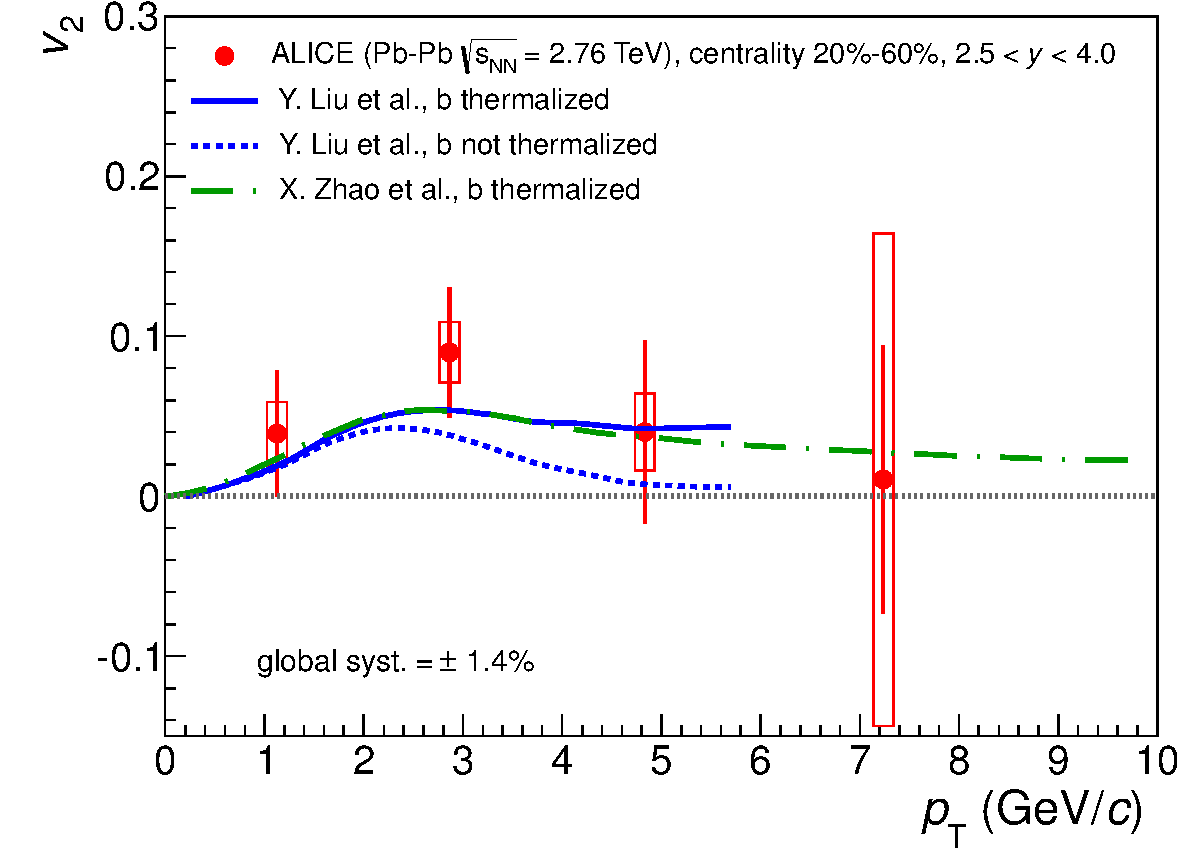
\includegraphics[width=0.49\linewidth]{quarkoniafigs/prl_fig4-eps-converted-to.pdf}
\label{fig:KS:v2ptcomp} 
\caption{Inclusive \jpsi\ \vtwo\
for \PbPb\ collisions with 20--60\% centrality at $\rootsNN = 2.76$\TeV\ as a function of \pT.
Also shown are the calculations from two transport models~\cite{Liu:2009gx,Zhao:2012gc}.
Reproduced from~\cite{ALICE:2013xna}}
\end{center}
\end{figure}

 Since, as discussed above, a fraction of \Jpsi\ originate from B-hadron decays, the results of model calculations depend on whether or not b quarks are assumed to be also thermalized. The model~\cite{Liu:2009gx} is presented for the two assumptions, showing a difference at higher \pt, where the B-decay fraction is larger and \Jpsi\ production by recombination is less important. The $v_2$ data prefer the version with thermalized b quarks, however, future precise measurements together with the access to higher \pt\ will shed more light on the question of b-quark thermalization. In addition, at high \pt\ initially produced \Jpsi\ in semi-central collisions may acquire a positive $v_2$ due to the different path length in the in-plane and in the out-of-plane directions, implying less dissociation in shorter in-plane path than in the out-of-plane direction. The various contributions can possibly be disentangled
by future precise studies of the \pT\ dependence of \Jpsi\ suppression and elliptic flow.

\subsection{Upsilon Suppression}

CMS measurements have provided the first high statistics data on \PgU\ production in heavy-ion collisions~\cite{CMS_Y_2010}. The three measured \PgU\ states have similar production and decay kinematics but different binding energies, and are therefore well suited to study in-medium heavy-quarkonium dissociation.
Uncertainties due to cold-nuclear-matter effects and to feed-down from higher mass states are less important for the \PgU\ family, compared to the situation of charmonium measurements. Since regeneration of \PgU\ states is presumed to be negligible, their suppression is expected to reflect pure dissociation processes. A complete understanding of the latter will also help the study of charmonia, where both mechanisms are present.

%Figure~\ref{fig:KS:mass} shows the invariant-mass spectra of $\mu^+\mu^-$ pairs produced in pp (left) and in Pb--Pb %(right) collisions obtained by CMS~\cite{Chatrchyan:2012lxa} at 2.76~TeV collision energy for both systems.
%For the \pp\ data, the excellent mass resolution of the CMS muon system
%allows a clear separation of the three \PgUn\ states. A similar mass resolution is achieved
%for \PbPb\ collisions.
Already the first invariant-mass spectra of $\mu^+\mu^-$ pairs produced in pp and in Pb--Pb collisions obtained by CMS~\cite{Chatrchyan:2012lxa} indicates
 a strong suppression of the \PgUb\ state is for \PbPb\ collisions, and the \PgUc\ state is even no longer visible above the combinatorial background. These results confirm the first \PgU\ measurement reported in~\cite{CMS_Y_2010}, and are in qualitative agreement with the expected \PgU\ suppression pattern as a function of the \PgUn\ binding energy.

%\begin{figure}[!ht]
%\begin{center}
%    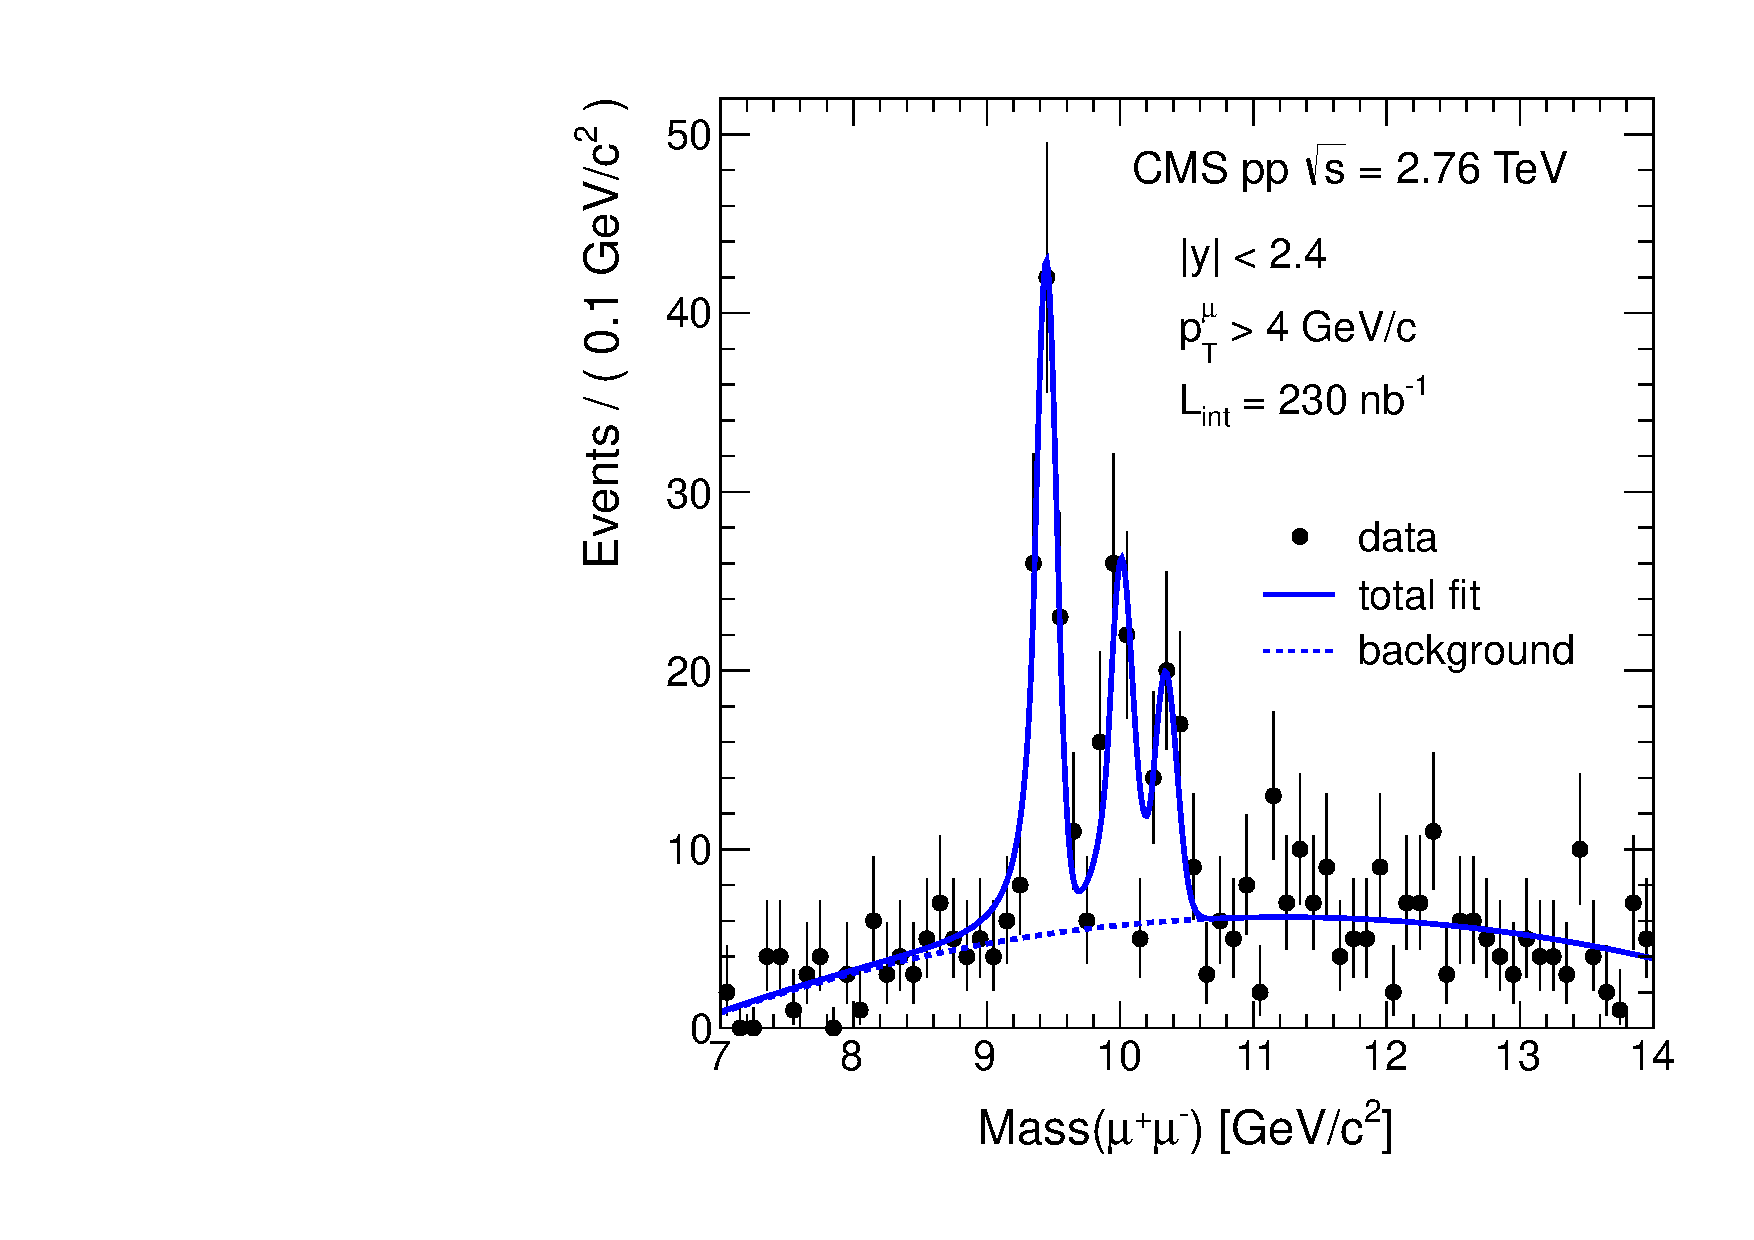
\includegraphics[width=0.45\textwidth]{quarkoniafigs/ppFitPt4Erf}
%    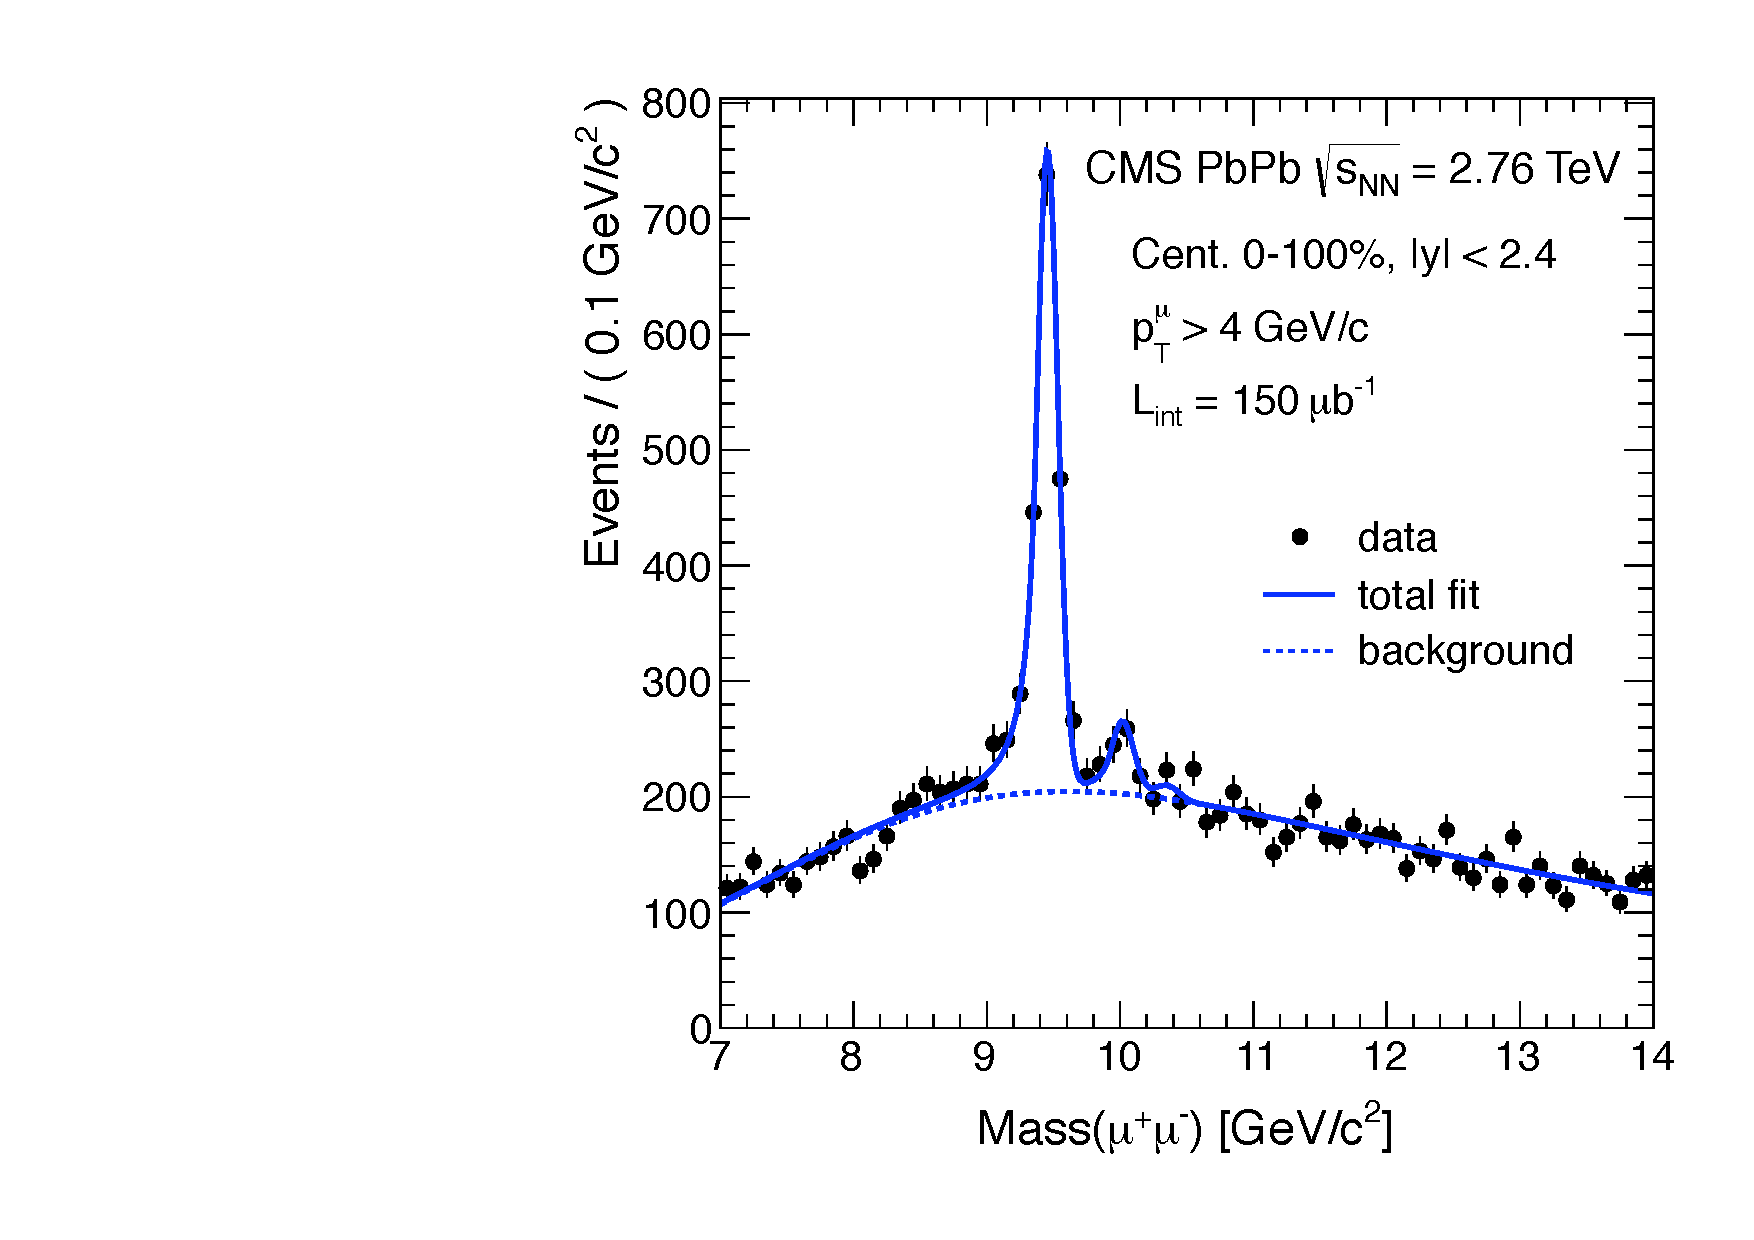
\includegraphics[width=0.45\textwidth]{quarkoniafigs/hiFitPt4Erf}
%    \label{fig:KS:mass}
%    \caption{Dimuon invariant-mass distributions in \PbPb\ (left) and \pp\ (right)
%at $\rootsNN = 2.76$\TeV. The lines show simultaneous fits to both
%data-sets for signal-and-background (solid) and background-only (dashed) contributions.
%Reproduced from~\cite{Chatrchyan:2012lxa}}
%\end{center}
%\end{figure}

From the \PbPb\ and \pp\ measurements the nuclear modification factor \Raa, characterizing the \PgU\ suppression,
can be calculated. The following centrality-integrated \Raa\ values were obtained for the different \PgUn states:
\begin{eqnarray}
\Raa (\PgUa) &=& 0.56 \pm 0.08\,\text{(stat.)} \pm 0.07\,\text{(syst.)} \,, \nonumber \\
\Raa (\PgUb) &=& 0.12 \pm 0.04\,\text{(stat.)} \pm 0.02\,\text{(syst.)} \,,  \\
\Raa (\PgUc) &=& 0.03 \pm 0.04\,\text{(stat.)} \pm 0.01\,\text{(syst.)} .  \nonumber
\end{eqnarray}
The statistical significance of the \PgUc\ signal is less than one standard deviation.
For the \PgUa\ state, there are significant feed-down contributions from the higher-mass bottomonia that may account for approximately 50\,\% of the yield~\cite{Affolder:1999wm, Aaij:2012se}.
This means that directly produced \PgUa\ state is probably largely unsuppressed, with
the observed \PgUa\ \Raa\ value essentially caused by the dissociation of the higher-mass excited states.


\begin{figure}[!ht]
\begin{center}
%   \includegraphics[width=0.45\textwidth]{qqbarfigures/chi2VsCent}
   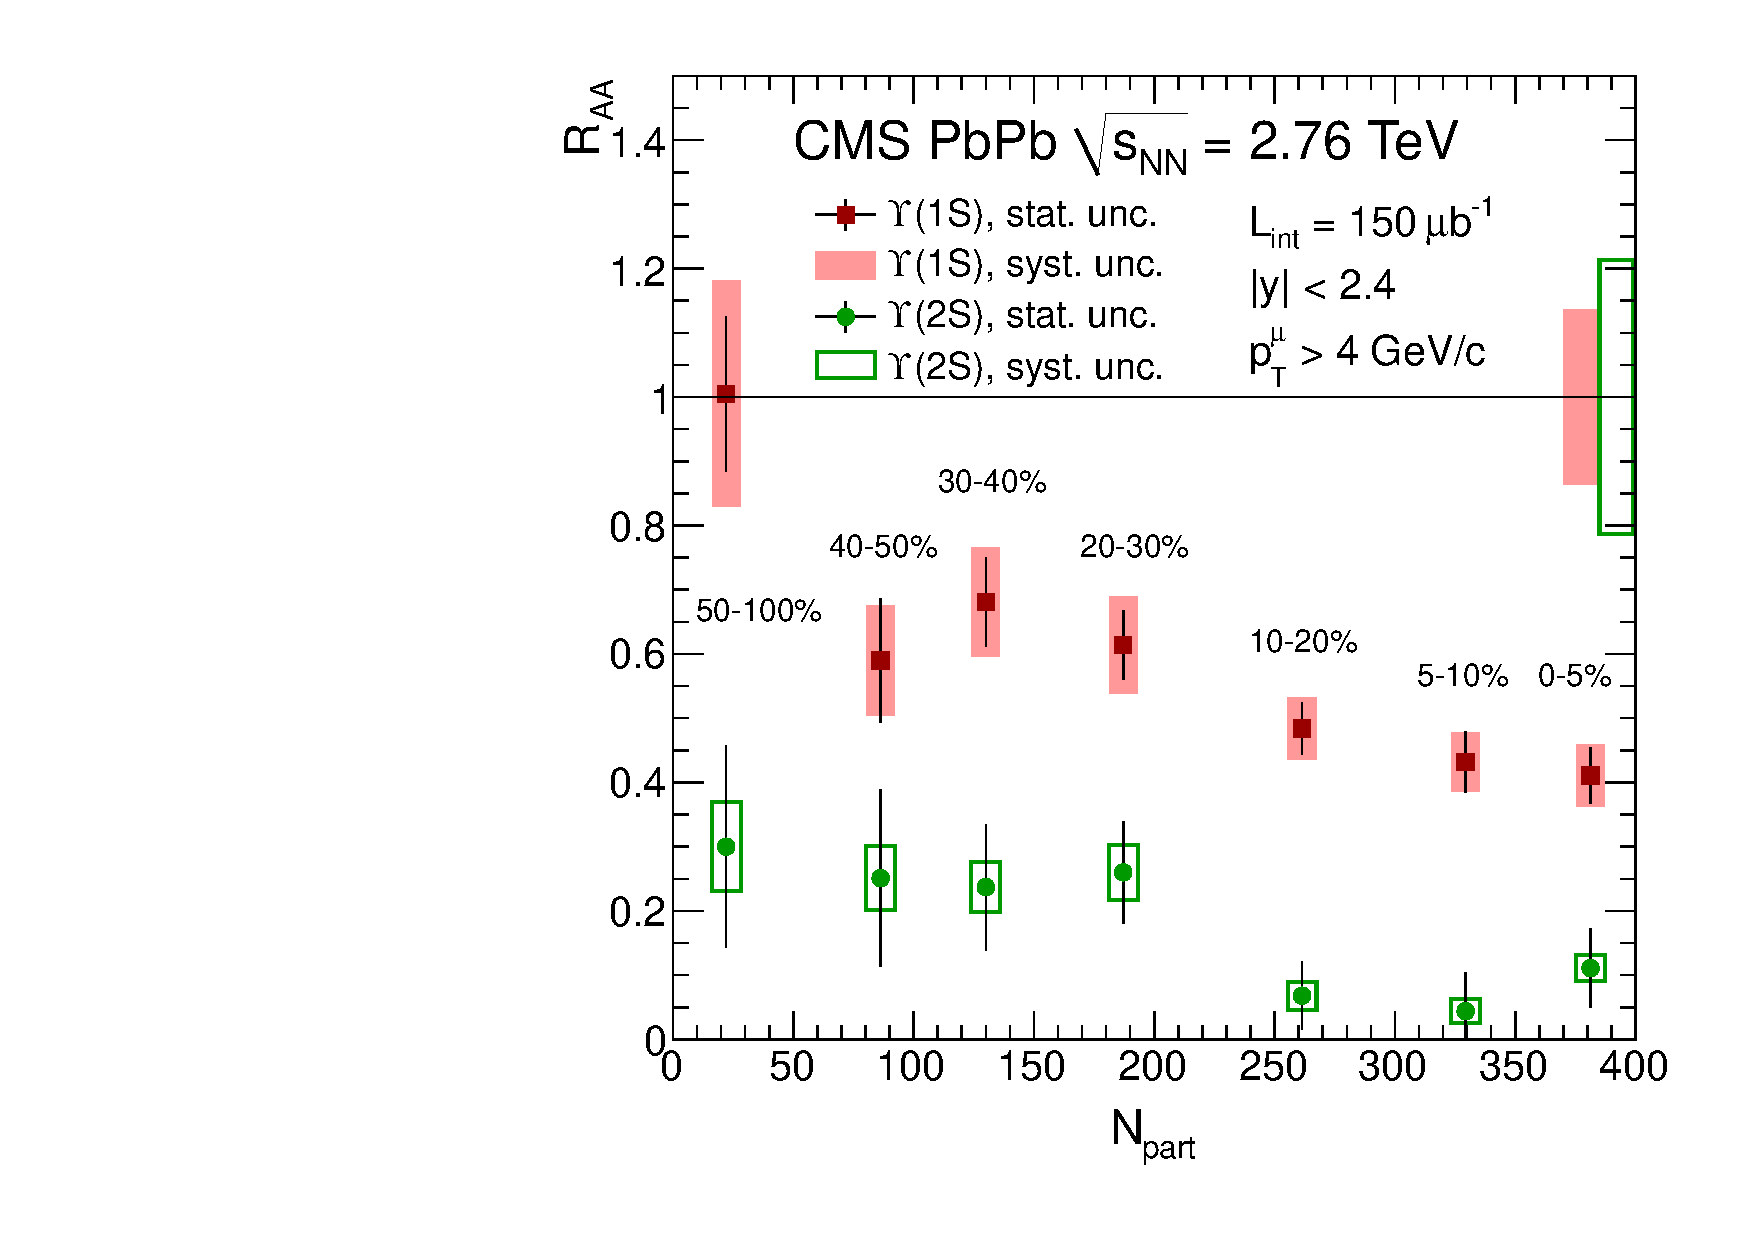
\includegraphics[width=0.49\textwidth]{quarkoniafigs/RaaPt4.pdf}
   \label{fig:KS:centrality}
  \caption{
%(Left): Centrality dependence of the \PgUa\ and \PgUb\ double ratios
%for 2.76\TeV\ \PbPb\ collisions.  (Right):
Nuclear modification factor \Raa\ for $\PgUa$ and $\PgUb$ as a function of $N_{\rm part}$ for $\rootsNN = 2.76$~TeV \PbPb\ collisions. Bars show statistical uncertainties, while the boxes around the points show systematic uncertainties. Common, centrality-independent uncertainties are represented by the boxes at unity. Reproduced from~\cite{Chatrchyan:2012lxa}}.
\end{center}
\end{figure}

The \PgUa\ and \PgUb\ suppression in terms of \Raa\ as a function of centrality expressed as $N_{\rm part}$
is shown in Fig.~\ref{fig:KS:centrality}.
%Here the relative suppression of \PgUa\ and \PgUb\ is characterized by
%the double ratio \linebreak $({\PgUb/\PgUa})_{\rm PbPb}/({\PgUb/\PgUa})_{\rm pp}$
%(Fig.~\ref{fig:GR:centrality}~(left) and the absolute suppression
%of the two states is shown as \Raa\ vs centrality (Fig.~\ref{fig:GR:centrality}~(right)).
The \Raa\ is strongly falling with increasing collision centrality
for both the \PgUa\ and the \PgUb, with a much stronger suppression for latter.
Overall, the data qualitatively exhibit the \PgUn\ suppression pattern
expected based on the hierarchy of binding energies. Although, the most peripheral bin
is rather wide (50--100\,\%), it is interesting to observe a strong suppression of the
\PgUb\ already for these centralities. 

ALICE and ATLAS are pursuing similar investigations of the \PgU\ family, and they have also presented their preliminary results.
Future high statistics \PbPb\ measurements
should elucidate the onset of the \PgU\ suppression in the most peripheral collisions,
in combination with information on \PgU\ production obtained from
studies of \pPb\ reference data, where the first results have been already reported.




\section{ELECTROWEAK BOSONS}
\label{sect:pas:ew}
%- Utility of penetrating probes
%- ALICE low pT photons measuring QCD temperature (cf. PHENIX)
%- Expected scaling of hard probes in A+B (nuclear thickness)
%- PDFs and nPDFs, calculation schemes (LO vs. NLO), codes
%- Z bosons (CMS first result cf. QCD), ATLAS Z centrality & rapidity
%- W (CMS published - can i compare to ATLAS prelim on a plot?)
%- Photon (CMS 2010, ATLAS prelim 2011?)

%While a primary topic in the study of heavy ion collisions is the modification
%of jets in the hot and dense nuclear medium, 
%Typical analyses of
%hard processes have assumed that the
%structure of a nucleon in a nucleus-nucleus collision is quantitatively the
%same as one in a nucleon-nucleon collision.
%From analyses of lepton-nucleus deep inelastic scattering data,
%it is known that cross sections do not scale linearly with the number of nucleons,
%as might be expected simply from the availability of scattering centers.
%The deviations from this scaling are referred to generally as ``nuclear shadowing'',
%and are typically shown as a function of Bjorken $x$ for different ranges in the
%hardness scale $Q^2$.
%The region around $x \sim 0.1$ corresponds to the valence quark region for a standard
%nucleon, and this is usually enhanced.  The region above this, $x \geq 0.2$ is typically
%suppressed (the so-called ``EMC effect''), while the region below $x << 0.1$ is also
%suppressed down to very small values of $x$.  The latter phenomenon is more
%typically known as ``nuclear shadowing'' and is thought to arise generally from
%quantum mechanical effects which deplete the numbers with small fractions of the
%nucleon momentum.

%It is important to understand the magnitude of these sorts of effects in
%the realistic environment of a heavy ion collision, in order to properly interpret
%measurements of hard process rates relative to a nucleon-nucleon reference system.
%At the RHIC collider, this was addressed early in the experimental program
%through measurements of high $\pT$ particles in deuteron-gold collisions.
%Presumably, any gross effects related to modifications of nucleon structure in the
%nuclear environment would show up as modifications in this system.  It was found that
%hadrons above $\sim 2$~GeV were produced at expected rates near $\eta =0$, confirming that
%the high $\pT$ suppression observed in the early days of the RHIC program did not
%arise from changes in nucleon structure, and strengthening the case for jet suppression
%in the hot and dense medium.
%However, it was also found that hadrons and J$/\psi$ particles were suppressed at
%forward angles, in the direction of the incoming deuteron, especially in more ``central''
%d+Au collisions, and enhanced slightly at backwards angles, in the direction of the
%nucleus.  These features are in broad agreement with predictions from calculations
%incorporating the nuclear shadowing observed in lepton-nucleus DIS.

%While the measurement of hadronic final states in proton (or deuteron)--nucleus collisions
%is thought to give useful information on modifications in the initial state of these
%simpler systems, the above-mentioned observed modifications of jets precludes similar
%observables giving similar information in heavy ion collisions.
%For this reason, great attention has been given to the measurement of
%``penetrating probes'', particles which do not interact strongly after they are produced.
%While charged leptons and neutral photons, of course,
%do not interact strongly, they come predominantly from
%jets and hadrons at relative low $\pT < 20$~GeV.
%However, at high $\pT$, most leptons are known to arise from the decay of electroweak
%bosons (Z and W particles).  Furthermore, isolated photons at high $\pT$ are predominantly
%``prompt'', i.e. arising from the direct interactions of quarks and gluons and not from
%electromagnetic decays of hadrons ($\pi^0$ and $\eta$).

While the production cross sections for heavy electroweak bosons are prohibitively small at the
top RHIC energies (200~GeV per nucleon-nucleon collision), the LHC provides the first
heavy ion system where all of the electroweak bosons are produced at substantial rates.
This section presents measurements of all three particles in \PbPb collisions at the LHC,
and shows their comparisons either with nucleon-nucleon reference data, or cross sections
calculated with perturbative QCD using standard structure functions.
The main physics goals of these measurements are 
to establish whether the production of the vector bosons is proportional to the
nuclear thickness or, equivalently, the number of binary nucleon-nucleon collisions,
and to see whether any modifications of vector boson production can be observed,
and if they can be attributed to modifications of the nuclear PDFs
Theoretical calculations provide some guidance as to the magnitude of the modifications
of standard PDFs expected in nPDFs, but substantial uncertainties remain due to the
different parameterizations of the existing nDIS data.
One feature which is predicted generically, however, is the decreasing magnitude of
nuclear modifications with increasing $Q^2$~\cite{Salgado:2011wc}.  
The large magnitude
of shadowing expected at low $Q^2$ (i.e. low \pT) is reduced substantially even by
$Q^2=100$~GeV.  
Thus, the large values of $M_{\mathrm Z}$ and $M_{\mathrm W}$ are already 80-90~GeV, 
naturally lead to nuclear modifications only at the 10-15\% level.

%\begin{figure}[!th]
%\begin{center}
%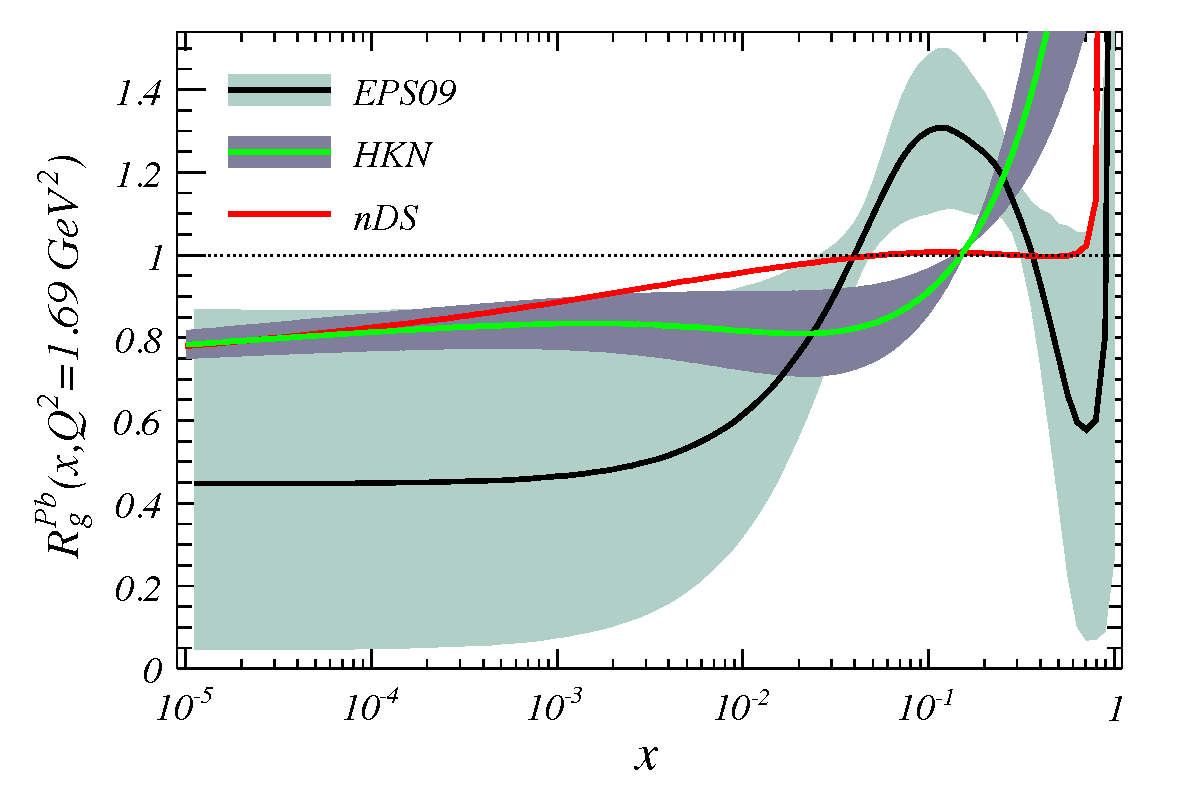
\includegraphics[width=0.49\textwidth]{electroweak_figs/gluonsnew.pdf}
%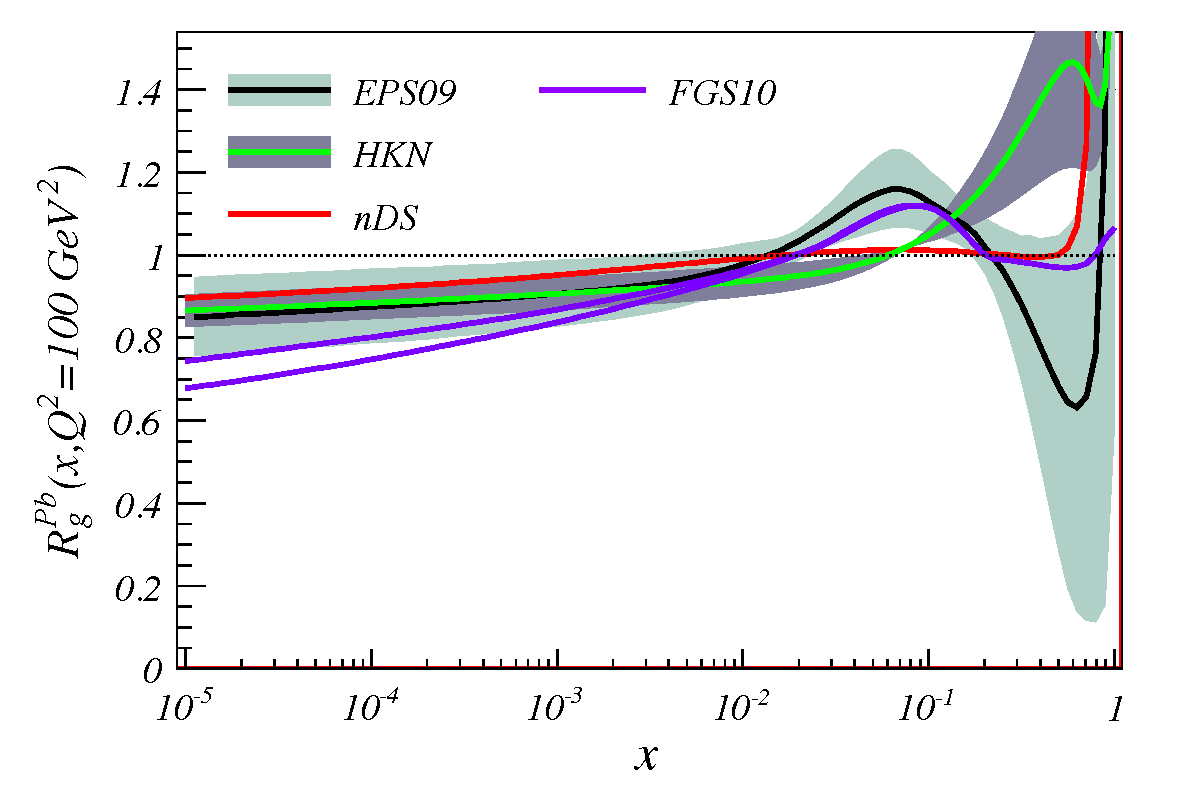
\includegraphics[width=0.49\textwidth]{electroweak_figs/gluonsnew100.pdf}
%\caption[]{
%(left) Modifications to proton PDFs expected from different nPDF implementations, for $Q^2=1.69$~GeV$^2$,
%(right) Modifications to proton PDFs expected from different nPDF implementations, for $Q^2=100$~GeV$^2$.
%From Ref.~\cite{Salgado:2011wc}.
%}
%\label{fig:pas:salgado}
%\end{center}
%\end{figure}

\subsection{W and Z bosons}

The first observation of vector bosons in \PbPb collision was performed by the ATLAS
experiment with a set of 38 Z candidates obtained in the first heavy ion run in 2010, which
was followed several months later by a CMS result comparing with theoretical calculations.
However, the statistical power of the 2010 sample was not sufficient to make strong conclusions
about the Z production rates as a function of the nuclear thickness.
The situation has improved dramatically with a published measurement of W bosons by CMS, also from the
2010 dataset, but benefiting from the large increase in the W cross section compared with Z.
ATLAS has also published the yield and spectrum of Z bosons from the much larger 2011 \PbPb dataset.
Together these give a relatively complete first look at the behavior of heavy vector bosons in
heavy ion collisions.


%\begin{figure}[!th]
%\begin{center}
%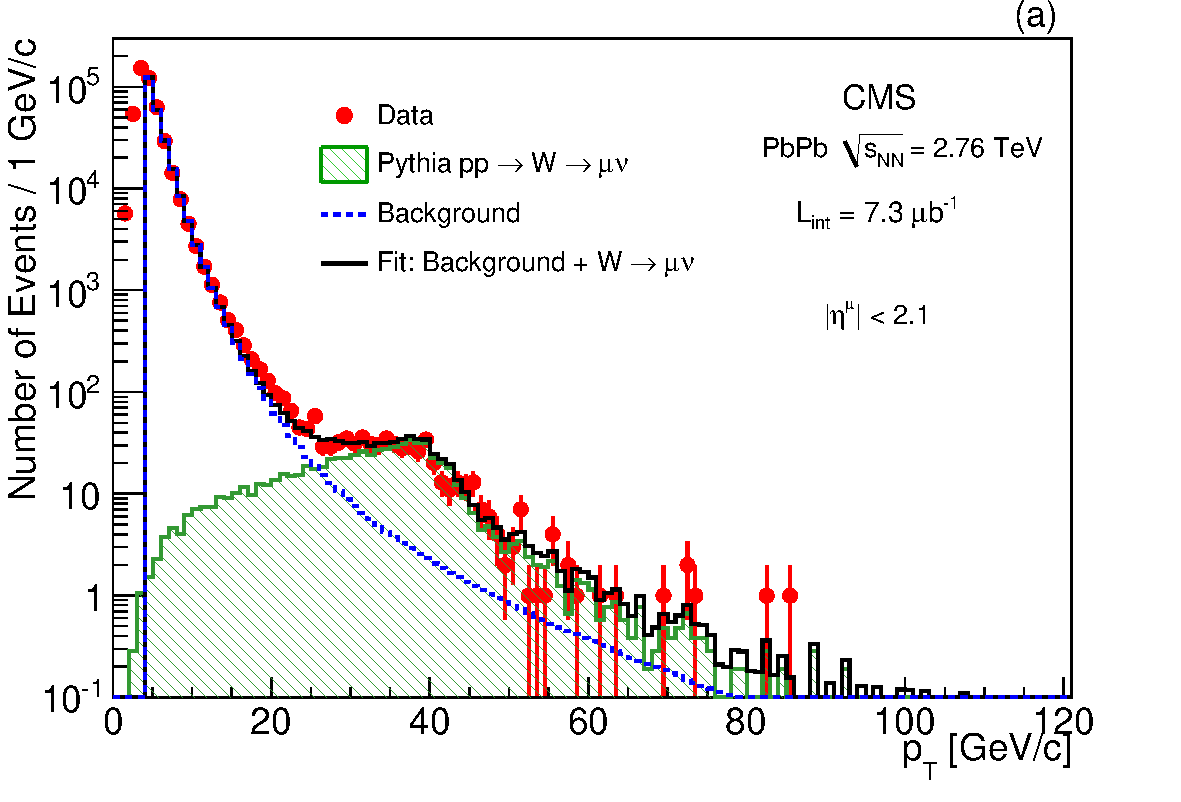
\includegraphics[width=0.49\textwidth]{electroweak_figs/Fig1a.pdf}
%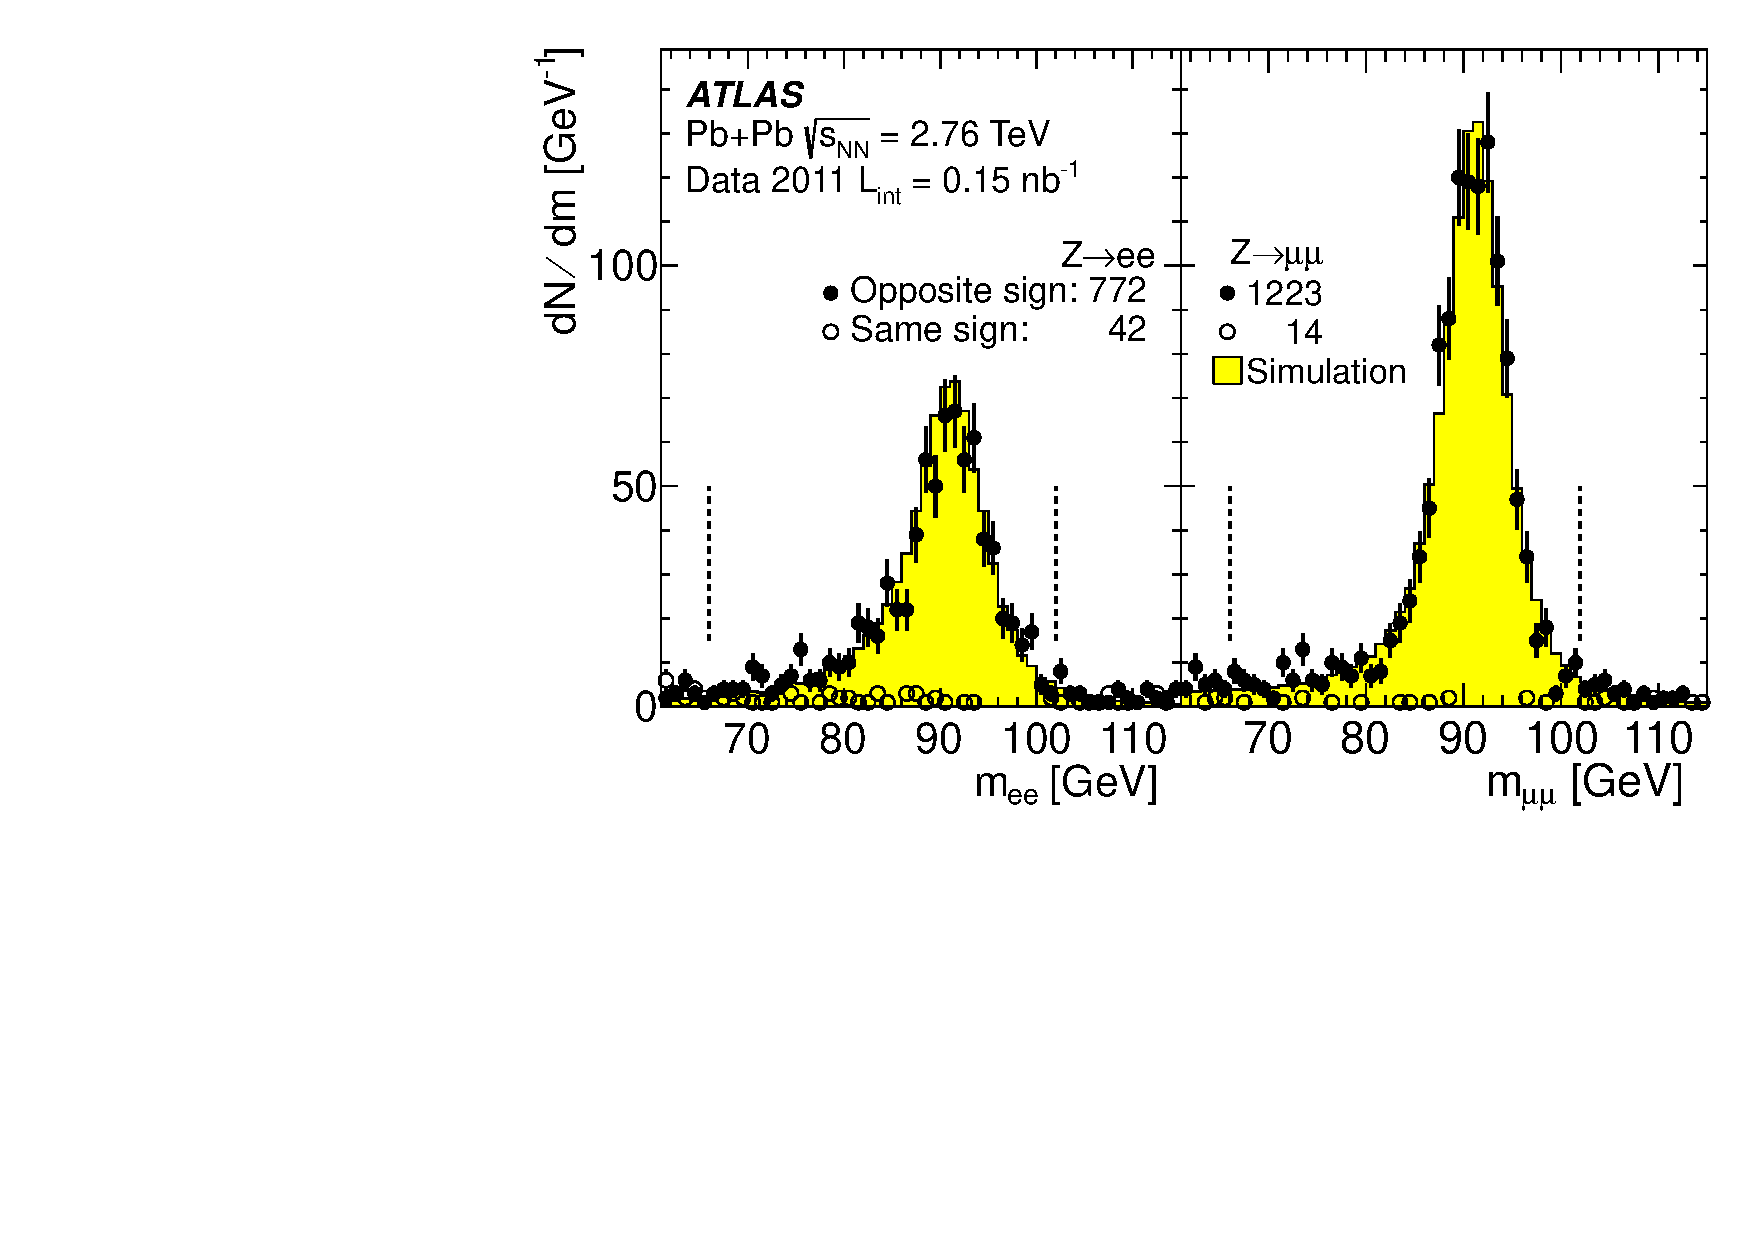
\includegraphics[width=0.49\textwidth]{electroweak_figs/fig_01.pdf}
%\caption[]{(left) Single muon spectrum, after selection cuts, from CMS data~\cite{Chatrchyan:2012nt} (right) Dimuon mass spectrum, in electron and muon channels from ATLAS data~\cite{Aad:2012ew}.}
%\label{fig:pas:zw_signal}
%\end{center}
%\end{figure}
The CMS W measurement was performed using the CMS inner tracker, which covers $|\eta|<2.4$
and the CMS muon spectrometer, which covers $|\eta|<2.4$ using a variety of gaseous detectors
(CSC, DT, with RPCs used for triggering), but was restricted to $|\eta|<2.1$ in this particular analysis.
The ATLAS Z measurement was performed combining dilepton decays in the muon and electron channels.
The ATLAS muon spectrometer uses drift tubes and cathode strip chambers to measure muons with $|\eta|<2.7$
in tandem with the ATLAS inner detector covering $|\eta|<2.5$.
Electrons are measured in ATLAS using the inner detector in association with the ATLAS calorimeter system,
which is particularly finely segmented in $\eta$ for $|\eta|<2.5$, allowing rejection of jet backgrounds.

%As shown in Figure~\ref{fig:pas:zw_signal}(left) from 
The CMS single muon spectrum at high $\pT$ clearly shows a contribution
%from W bosons as a peak near 40~GeV.
The backgrounds from jets are strongly reduced by calculating the missing $\pT$ for each event with a
high \pT muon, based on tracks with $\pT>3$~GeV.  The background from Z bosons is removed by removing muons which
combine with a second muon in the same event that reconstructs to a mass near the Z mass.
After selections, about 540 W candidates were found in the 2010 \PbPb data.
%
%Figure~\ref{fig:pas:zw_signal}(right) shows the dimuon and dielectron mass spectrum after requiring $\pT>10$~GeV for
%the muons, and $\pT>20$~GeV for the electrons.  
The ATLAS Z lineshape is in good agreement with simulations for both
dielectron and dimuon channels.
After selections, about 2000 Z candidates were reconstructed in the 2011 ATLAS \PbPb data.

\begin{figure}[!th]
\begin{center}
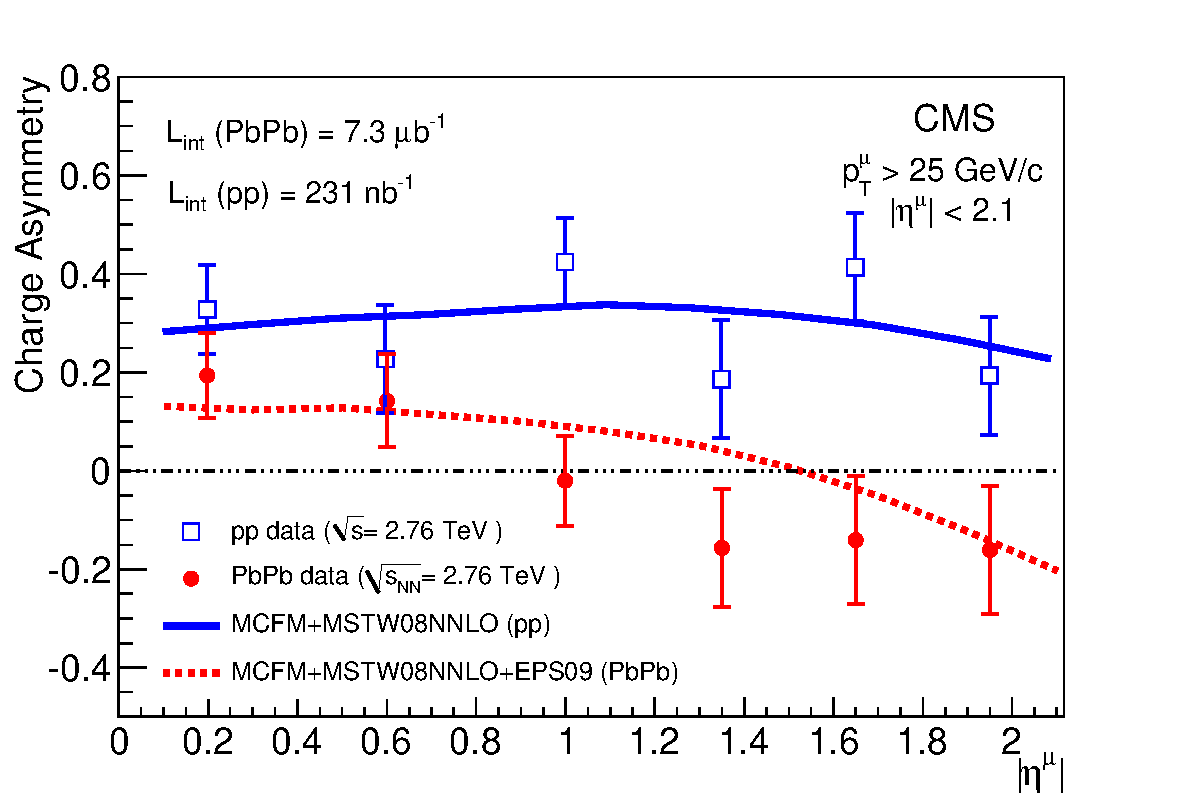
\includegraphics[width=0.49\textwidth]{electroweak_figs/Fig3.pdf}
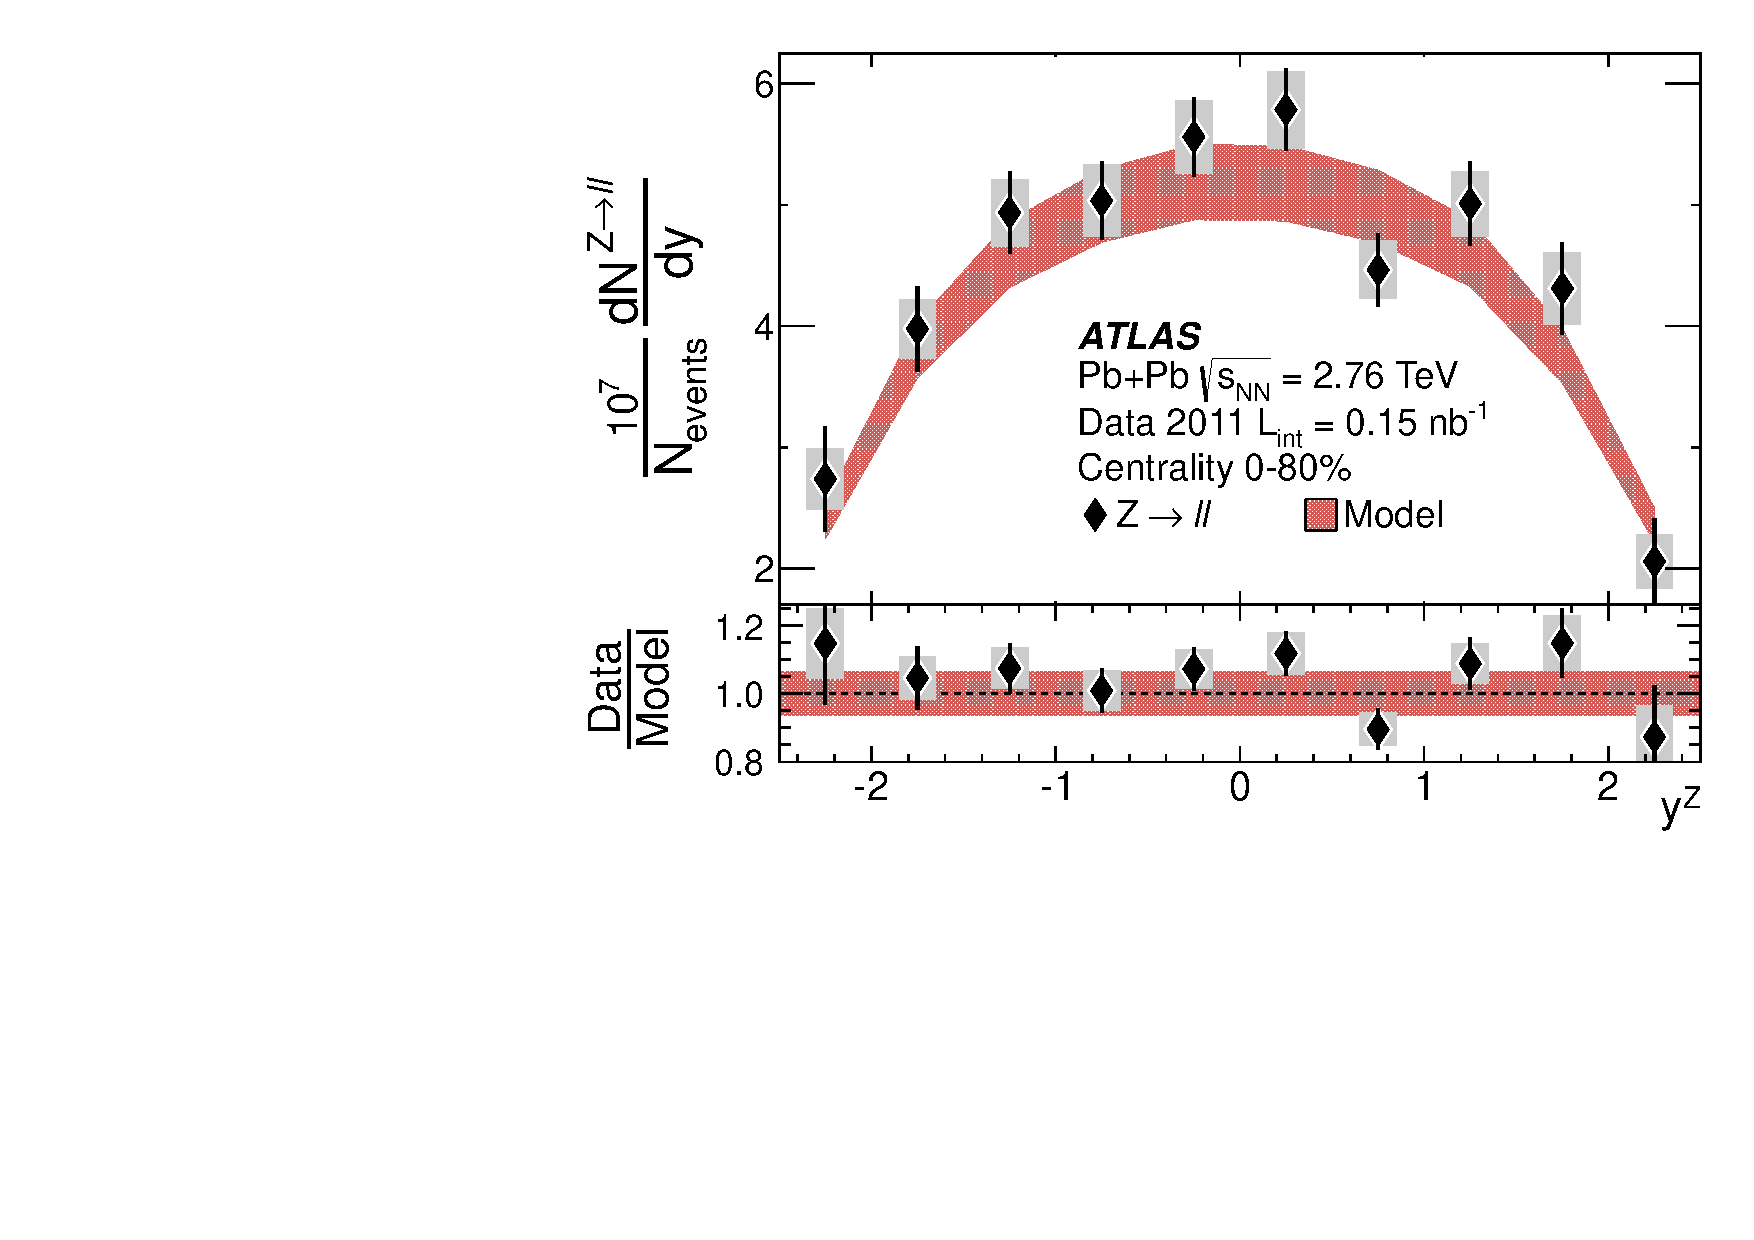
\includegraphics[width=0.45\textwidth]{electroweak_figs/fig_02.pdf}
\caption[]{(left) Charge asymmetry for W candidates, from CMS data~\cite{Chatrchyan:2012nt} (right) Rapidity dependence of $dN_{\mathrm{Z}}/dy$ compared to PYTHIA scaled to the NNLO cross section~\cite{Aad:2012ew}}
\label{fig:pas:zw_eta}
\end{center}
\end{figure}
Figure~\ref{fig:pas:zw_eta}(left) shows the pseudorapidity dependence of the charged lepton asymmetry for the muons associated with
the CMS
W candidates ($A_\mu = (N_{\mathrm{W}^+}-N_{\mathrm{W}^-})/(N_{\mathrm{W}^+}+N_{\mathrm{W}^-})$), both for \PbPb and \pp data at the same CM energy
($\sqrt{s_\mathrm{NN}}=2.76$~TeV).  The evident differences between the \PbPb and \pp stem primarily from the neutrons in the
Pb nuclei, which modify the expected charge distribution, particularly in the forward direction where the Bjorken $x$ probed
is sensitive to the valence quarks.
Both data sets are compared with NNLO calculations of the W charge asymmetry and good agreement is found for both \pp and \PbPb.
While this suggests that no large nPDF effects are needed to accommodate the existing data, it was pointed out in Ref.~\cite{Paukkunen:2010qg}
that the scale factors in EPS09 formalism will cancel out in the charge asymmetry ratio, making this quantity suboptimal for
isolating nPDF modifications.

Figure~\ref{fig:pas:zw_eta}(right) shows the rapidity dependence of the per-event
Z boson yield in the 0-80\% centrality interval in \PbPb collisions
from the 2011 ATLAS \PbPb data.
The data is compared to the same distribution from PYTHIA (version 6.425), scaled to the NNLO total cross section,
and the appropriate mean nuclear thickness.
Good agreement is found between the heavy ion data and the absolutely-scaled PYTHIA reference, the ratio between them being consistent
with unity within the stated uncertainties.  
While small effects at the 10-15\% level are not ruled out, nor are they required to
make sense of the current measurements.

\begin{figure}[!th]
\begin{center}
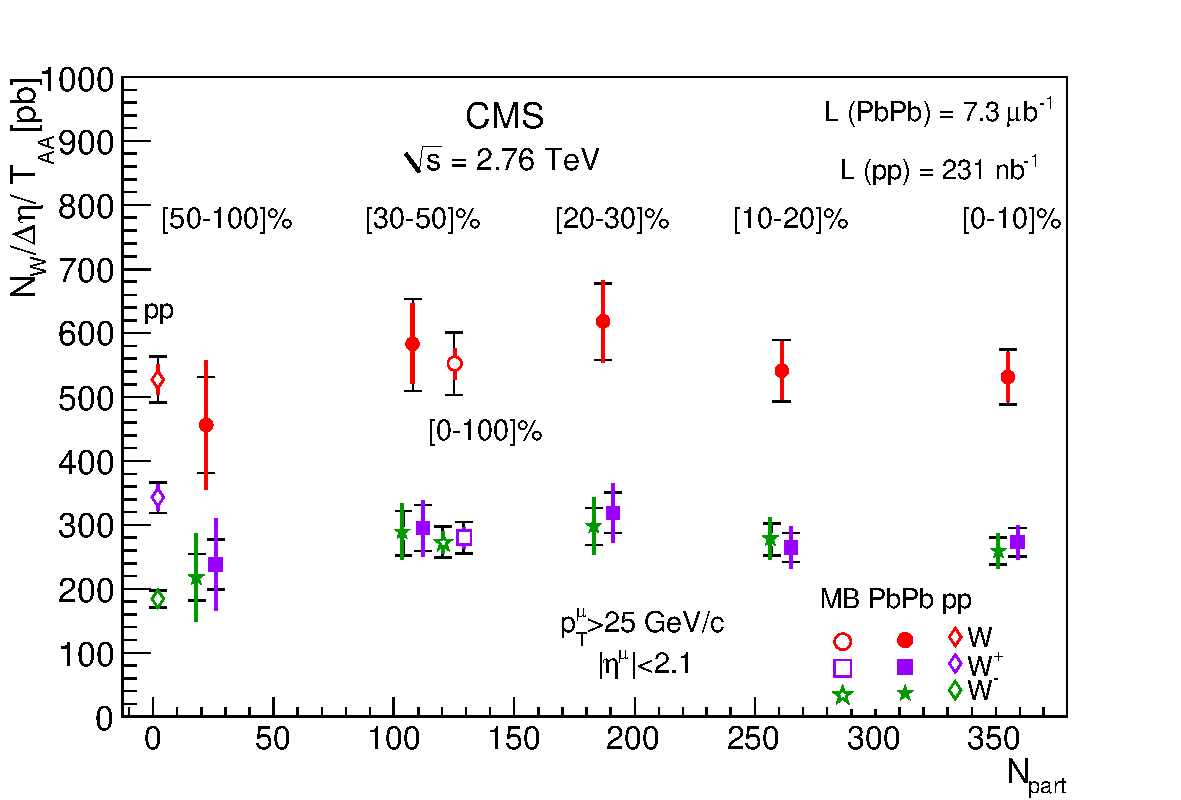
\includegraphics[width=0.54\textwidth]{electroweak_figs/Fig2.pdf}
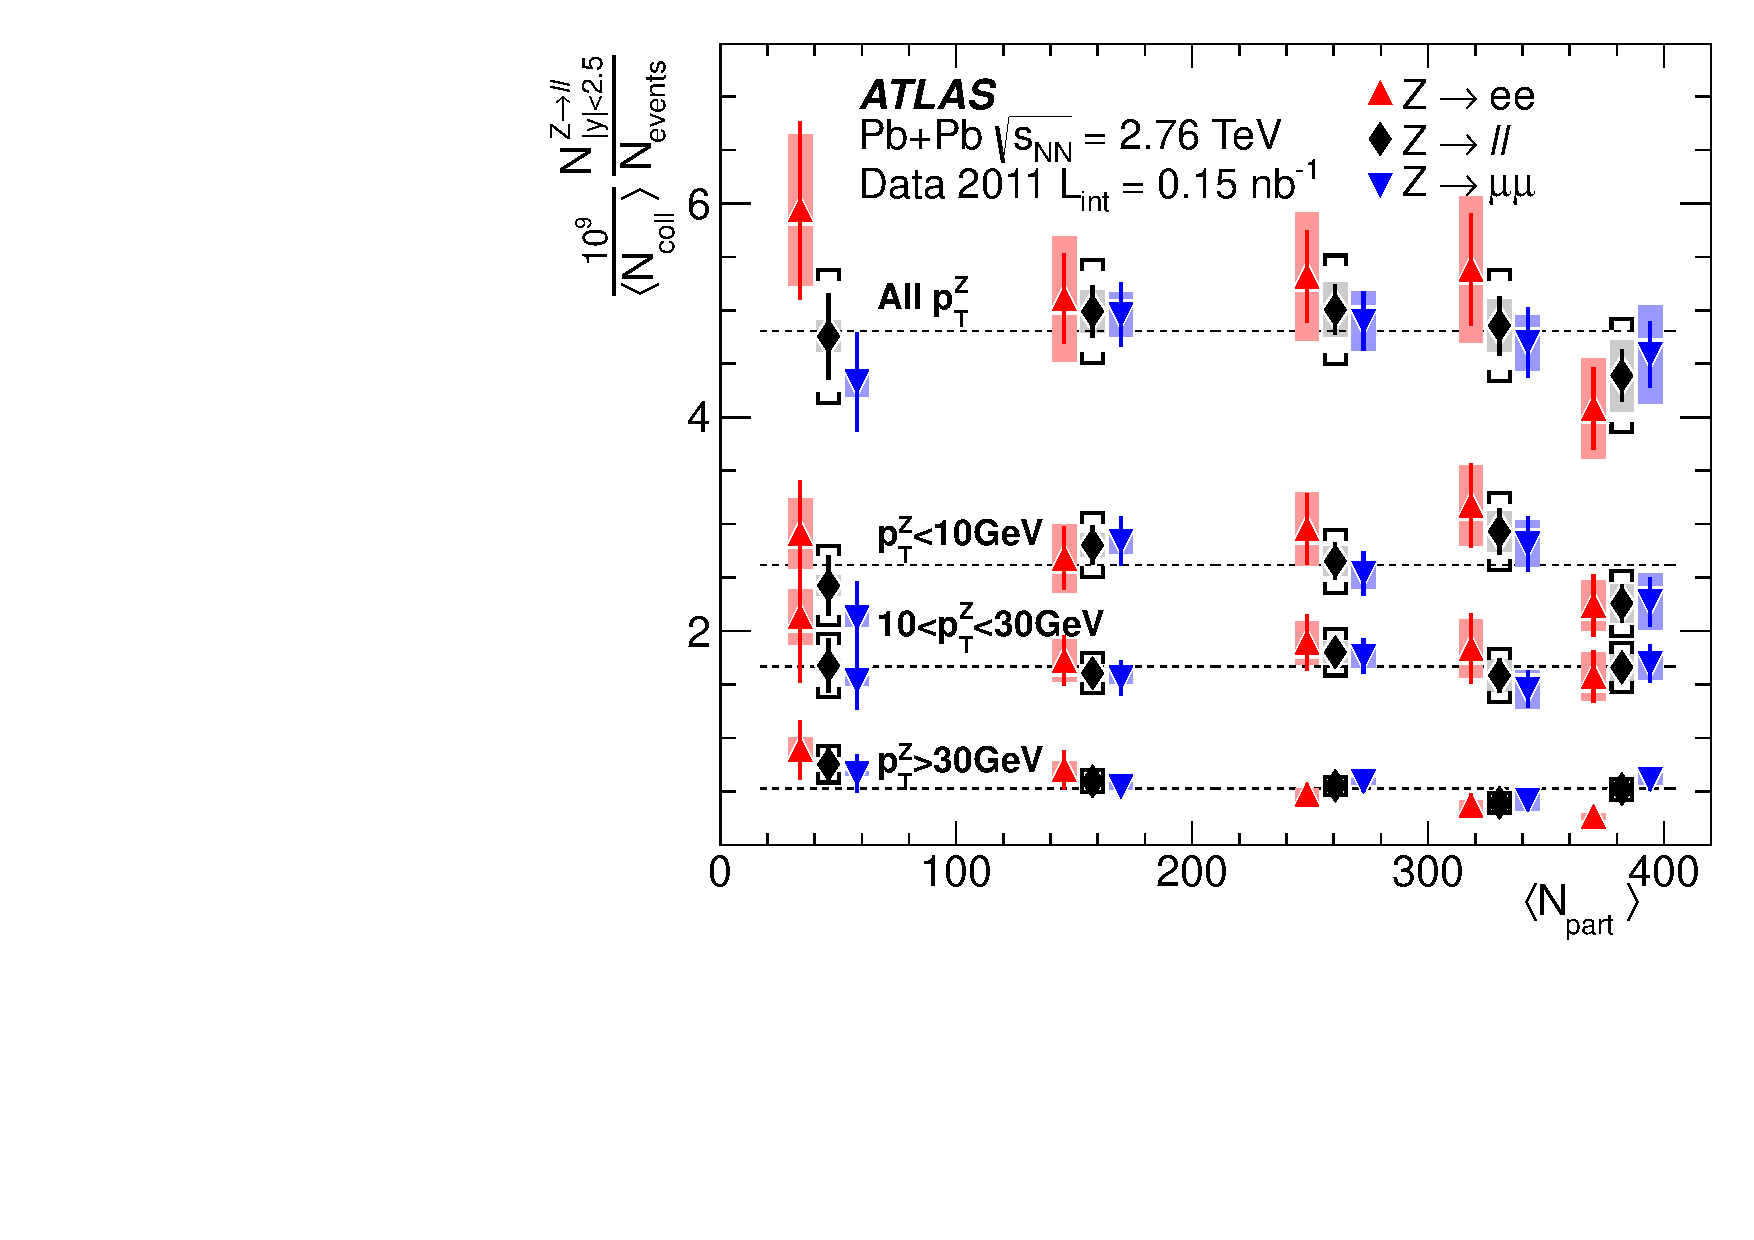
\includegraphics[width=0.44\textwidth]{electroweak_figs/fig_04.pdf}
\caption[]{(left) Yield per collision for W candidates, from CMS data~\cite{Chatrchyan:2012nt} (right) Yield per collision for Z's, in both electron and muon channels from ATLAS data~\cite{Aad:2012ew}.}
\label{fig:pas:zw_cent}
\end{center}
\end{figure}

The centrality dependence of the separate W charge states and the total from CMS
is shown in Figure~\ref{fig:pas:zw_cent}(left),
as a function of the number of participating nucleons, and for the \pp data.
While \pp shows a clear difference between positive and negative W's, reflecting the charges of the initial protons, there is little
difference between them in the \PbPb data, reflecting the additional down quarks introduced via the neutrons in the Pb nuclei.
The heavy ion data shows a clear scaling with centrality, once the W yields -- both for the charge-separated yields, and the
total -- are scaled by the number of binary collisions.
A similar message is found in the ATLAS Z data, shown in Figure~\ref{fig:pas:zw_cent}(right), which shows the Z yield, scaled by
the number of binary collisions, also as a function of the number of the mean number of participating nucleons for each
centrality interval.  The ATLAS data also shows that the centrality dependence is the same for the dielectron and dimuon channels,
and even for selected intervals in the Z \pT.

\subsection{Photons}

\begin{figure}[!ht]
\begin{center}
\raisebox{5mm}{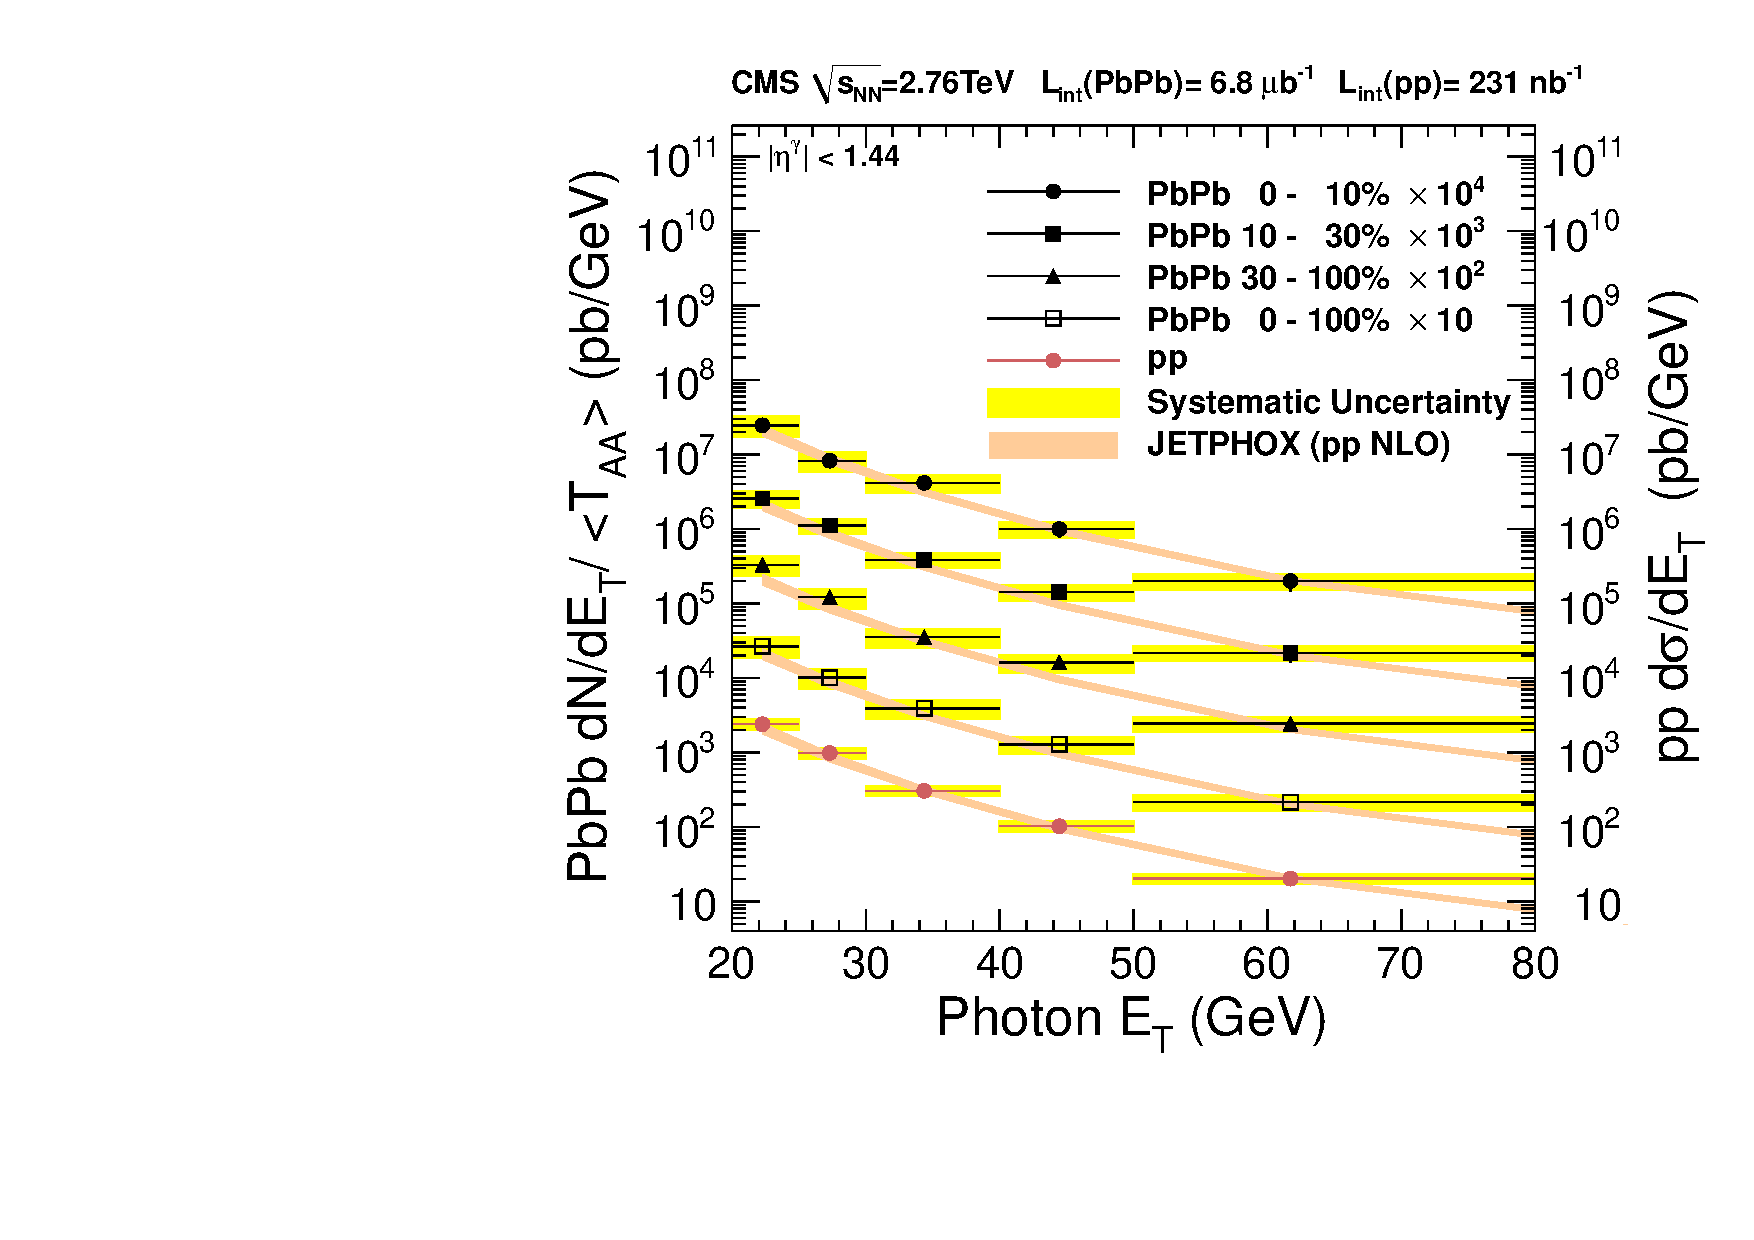
\includegraphics[width=0.50\textwidth]{electroweak_figs/TAAScaling.pdf}}
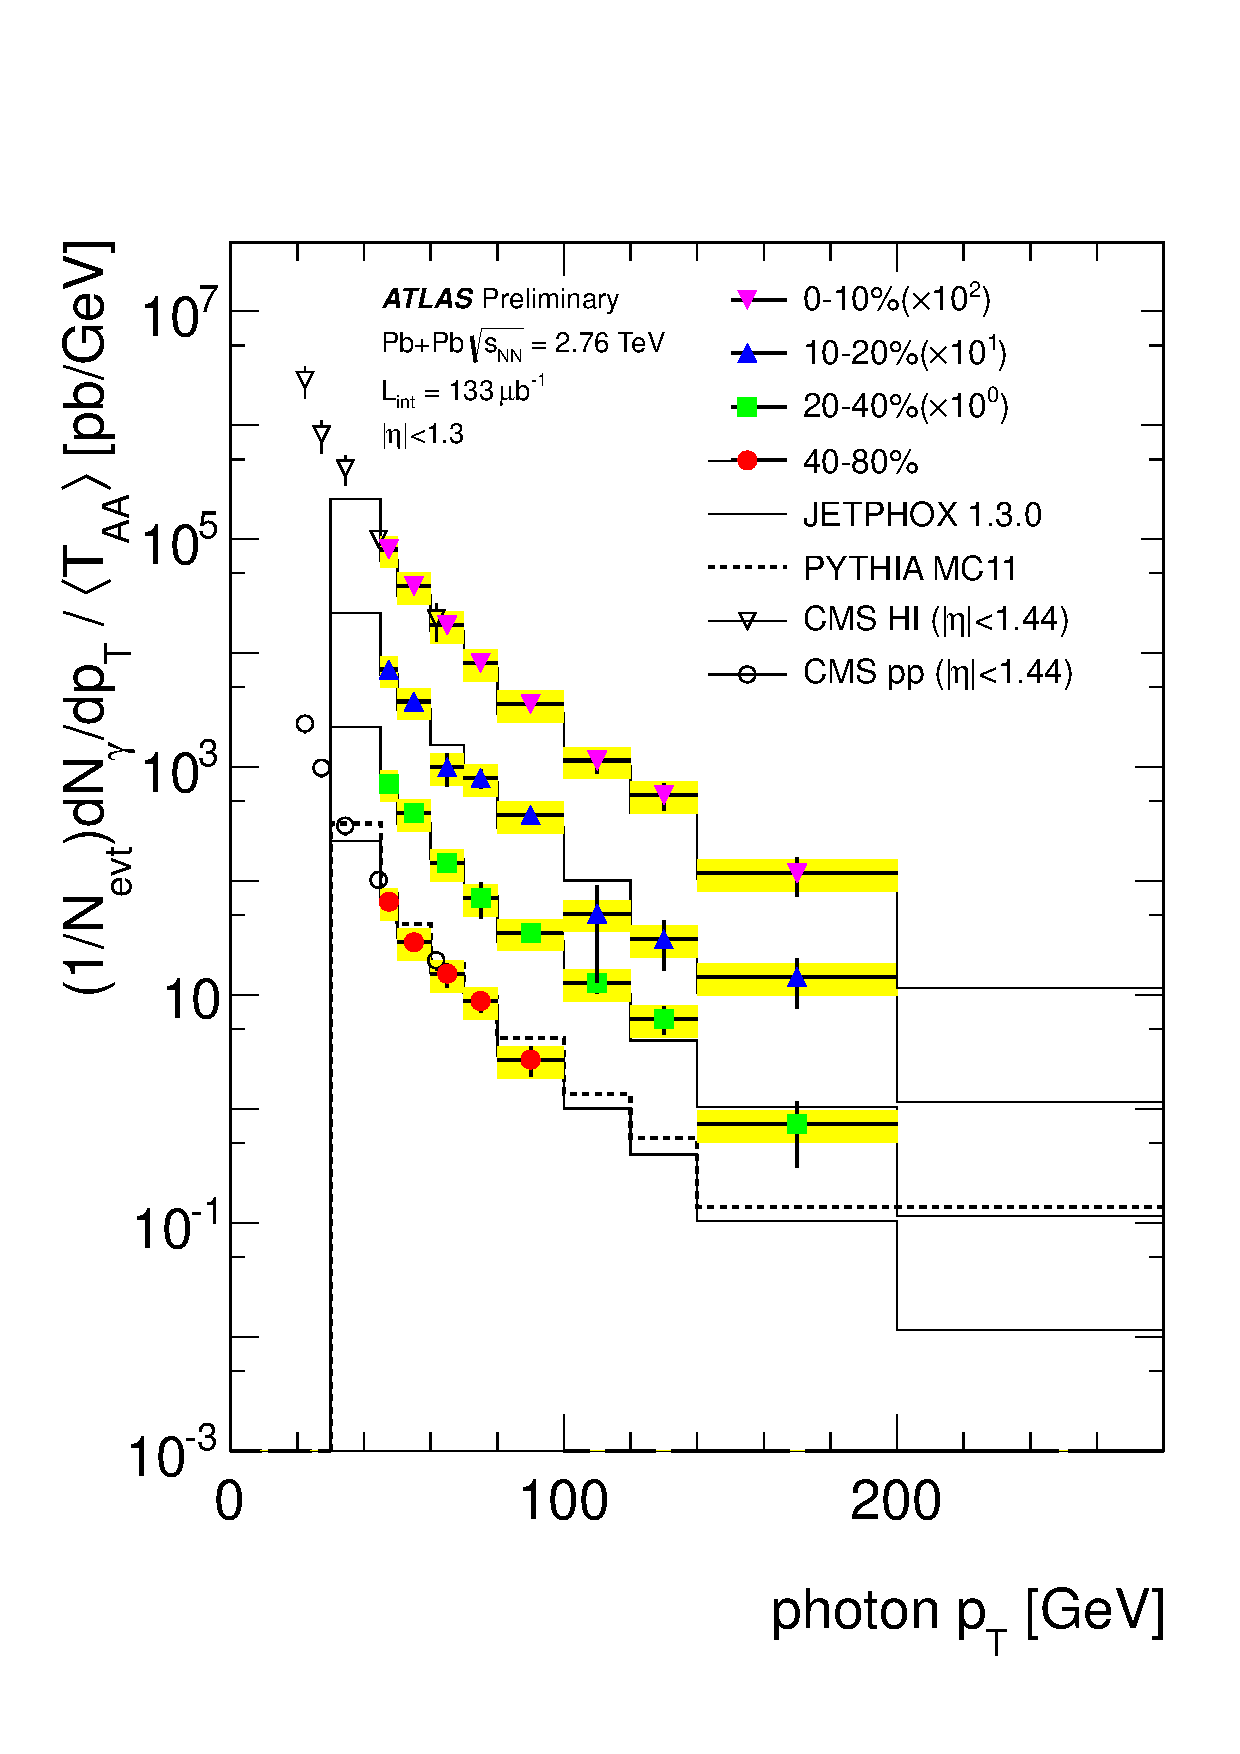
\includegraphics[width=0.40\textwidth]{electroweak_figs/ph_fig_11.pdf}
\caption[]{(left) Photon yields scaled by the mean nuclear thickness function for $|\eta|<1.44$, from CMS data~\cite{Chatrchyan:2012vq} (right) The similar quantity from ATLAS, for $|\eta|<1.3$, from ATLAS data~\cite{ATLAS:2012zla}.}
\label{fig:pas:photon}
\end{center}
\end{figure}

The measurement of photons in heavy ion collisions is also an important contribution to the
study of the \PbPb initial state.
%, with some advantages and disadvantages.  Unlike Z and W bosons,
%no energy from the initial 2-to-2 scattering process is used in the boson mass,
%and so the cross sections at high \pT\ are substantially higher at the same transverse momentum.
%However, photon measurements do not provide a clear mass peak, and nor are they associated with
%a track measured in an inner tracker.  This means that backgrounds are an irreducible part of
%the measurement, particularly at low \pT, where one expects large contribution from jet fragmentation
%into high momentum neutral pions or eta mesons.

%At low \pT, ALICE has performed a preliminary measurement of the spectrum of direct photons
%using the so-called ``subtraction'' method~\cite{Wilde:2012wc}.
At low \pT, ALICE has measured inclusive photons
and the contribution from hadron decays is estimated through a combination of direct measurements
and a cocktail based on $m_{\rm T}$-scaling.
%Using this, the remaining contribution from direct photons is extracted and compared to
%perturbative QCD calculations.  This has been performed on 7~TeV \pp data, and good agreement
%with pQCD is found.  
In the 0--40\,\% centrality interval in \PbPb, good agreement is found above
$\pT=4$~GeV with a scaled NLO calculation at the \PbPb CM energy.  However, an excess is observed
below 4~GeV, which is fit by an exponential and gives an inverse slope parameter of
$T_{\mathrm{LHC}} = 304 \pm 51^{\mathrm{syst+stat}}$ MeV.  By comparison to a similar
measurement from PHENIX, which observes an inverse slope of
$T_{\mathrm{PHENIX}}=221 \pm 19^{\mathrm{stat}} \pm 19^{\mathrm{syst}}$ MeV for the 0-20\%
centrality interval at the top RHIC energy~\cite{Adare:2008ab},
ALICE concludes that the initial temperature at the LHC is higher
than that measured at RHIC.

%At high \pT, two primary techniques are used to increase the purity of the photon sample, which is typically
%$O(0.1\%)$ based on the expected relative yields of photons and jets.  The first is to select
%photon candidates as electromagnetic clusters which pass a set of selection criteria, trained on
%photon simulations to efficiently reject electromagnetic decays while keeping most of the
%produced photons.  These criteria involve both the ``shape'' of the cluster (since photon showers
%are typically quite narrow), as well as the presence of energy in the ``hadronic'' section of the
%experimental calorimeters (since photon showers should typically be well-contained in the front
%electromagnetic sections).
%The second technique is to require that the photon candidate is ``isolated'', i.e. only a limited
%amount of ambient energy, including both electromagnetic and hadronic contributions,
%is allowed to be present near the photon.  In the context of a heavy ion collision, where there
%is typically a substantial amount of uncorrelated energy present, techniques must be applied to
%estimate and remove this energy event by event.  However, even after doing this, one must account
%for real photons with an upward fluctuation of ambient energy nearby (``leakage'') as well
%as fake photons with a downward fluctuation, passing the nominal selection criteria.
%Thus, shower-shape discriminators are typically combined with an isolation requirement, and various
%means exist to combine this information to estimate the true purity of a photon sample in a
%data-driven fashion.

At higher \pT, 
the CMS photon measurement is performed using electromagnetic clusters in the CMS ECAL, with the
CMS tracks and HCAL used to tag backgrounds from electrons or hadronic decays.
The signal from prompt isolated photons is extracted using a two-component template fit to
the distribution of $\sigma_{\eta\eta}$, a variable which reflects the width of the cluster
in the $\eta$ direction.  
%The signal is derived from PYTHIA $\gamma$+jet events, embedded
%into real \PbPb\ data events.  The background distribution is derived from a set of photon
%candidates which are required to fail the isolation selection.
%After subtracting the extracted backgrounds and correcting for efficiency and resolution
%effects, the yield of photons is presented as a function of \pT in three centrality intervals
%as well as a minimum-bias (0-100\%) interval.  A similar analysis performed on \pp\ data is
%also shown.
In Figure~\ref{fig:pas:photon}(left),
both the heavy ion and pp data are compared with an NLO pQCD calculation (using the
JETPHOX package) by scaling the calculation by the mean nuclear
thickness function $\langle T_{\mathrm{AA}} \rangle$ relevant for each interval.
It is found that the NLO calculations agree with the pp and heavy ion data in all cases, within
the stated statistical and systematic uncertainties.  This demonstrates that, like the
Z and W results, the photon yields scale with the number of binary collisions.
However, while the Z and W results focused on integrated yields, the photons show that
there is also no modification of the spectral shape.
ATLAS performed a similar analysis, using the ``double sideband'' technique to estimate the
photon fraction in each \pT and centrality interval for $|\eta|<1.3$.
In Figure~\ref{fig:pas:photon}(right), the preliminary ATLAS data is shown compared with both
the CMS data and JETPHOX 1.3.0 results.  The ATLAS and CMS data agree well (given the 5\%
difference in the $\eta$ range) and ATLAS data agree with JETPHOX out to $\pT = 200$~GeV.



\section{JET SUPPRESSION}
\label{jets}
Unlike the production of electroweak bosons, which is observed to be essentially described by
an independent superposition of nucleon-nucleon collisions within current experimental uncertainties,
jet production is substantially modified in high energy heavy ion collisions.
%The first indications of this were observed by all four major experiments at the RHIC collider.
%The rates of high transverse momentum ($\pT>4$ GeV) particles emitted in Au+Au collisions
%were found to be suppressed
%by a factor of approximately 5 relative to the rates predicted using the number of binary
%collisions, something not seen in d+Au collisions (ruling out strong nPDF effects).
%Correlations of high momentum particle pairs (typically referred to as ``trigger'' and ``associated''
%particles) also showed a distinctive signature of the disappearance
%of back-to-back associated particle emission in Au+Au up to trigger $\pT \sim 8$ GeV, 
%again something not observed in d+Au.
The RHIC experimental program did not have the large acceptance detectors or the large jet rates 
available at the LHC, and so jet measurements have been particularly challenging and no 
published results are available.
Jets are measured by all three large LHC experiments.  ATLAS and CMS are similar in that they
have large acceptance ($|\eta|<5$) hadronic and electromagnetic calorimetric coverage, and 
precise silicon trackers ($|\eta|<2.4$ for CMS and $|\eta|<2.5$ for ATLAS), 
both of which are used in jet measurements.
%ATLAS primarily relies on calorimetric jet measurements, grouping smaller readout ``cells''
%into towers of angular size $\Delta \eta \times \Delta \phi = 0.1 \times 0.1$. 
%The anti-$k_t$ jet clustering algorithm is used to partition the towers into proto-jets
%and exclude towers in regions with large localized energy depositions.  The remaining towers
%are then used to estimate the uncorrelated background as a function of $\eta$, including
%an estimate for an overall azimuthal modulation due to elliptic flow.  This background is subtracted
%cell-by-cell in each calorimeter 
%layer from all remaining jet candidates and then the background estimated again after excluding
%jets with $E_T>25$ GeV.  After this second step the background is subtracted again from all
%jets, and the final jet kinematics are recalculated using the subtracted cells.
%CMS also uses an iterative procedure based on calorimeter towers.  For each $\eta$ ring
%of $\Delta \eta \sim 0.87$, the average transverse energy and standard deviation are calculated
%for each event and $\langle E_T \rangle + \sigma$ are subtracted from each event, and negative
%values are set to zero.  Jets are then found using an iterative cone algorithm, the tower background
%recalculated after excluding jets of at least 30 GeV, and the final jets are reconstructed 
%on the subtracted towers.
ATLAS primarily relies on calorimetric jet measurement, grouping smaller readout ``cells''      
into towers of angular size $\Delta \eta \times \Delta \phi = 0.1 \times 0.1$, and 
clustering them with the anti-$k_t$ algorithm with varying cone size.
CMS uses both a seeded cone algorithm and a 
particle flow technique, providing tracks and calorimeter objects to the 
anti-$k_t$ algorithm with $R=0.3$.
ALICE has much smaller angular coverage and so no published full jet results are available.

\subsection{Dijet correlations}

The first result on jets at the LHC was released by the ATLAS collaboration 
several weeks after first collisions were seen by the three main experiments.  
ATLAS performed a measurement~\cite{Aad:2010bu} of
the asymmetry between the two highest-energy jets in events with at least one jet
with $E_{T1} > 100$ GeV, and a second jet $E_{T2} > 25$ GeV.  The asymmetry is
then defined as $A_J = (E_{T1} - E_{T2})/(E_{T1} + E_{T2})$.
Figure~\ref{fig:pas:final_4x2} shows the evolution of the distribution of
$A_J$ with collision centrality, compared to both proton-proton data at 7 TeV
as well as a full simulation of events where PYTHIA dijets are embedded into
Pb+Pb events generated by HIJING.
It is observed that while the distributions in the 40-80\% most central events
resemble the simulated events and the pp data, the $A_J$ distribution becomes
progressively wider in the more central events, indicating an increasing attenuation
of the energy of the second jet relative to the leading jet.  This is generally
understood to be a direct observation of jet quenching, where the jet loses energy
in the hot and dense medium.
%While the RHIC results generated a wide range of theoretical descriptions, the reliance
%on leading particles precluded strong statements about the nature of the energy
%loss process, whether it was from the inducement of a single hard radiative gluon
%from the primary, or from many soft radiations.
The lower row on the ATLAS figure already indicated that the energy loss could not be
from single hard emissions since the back-to-back pattern observed in pp and in
the most peripheral sample was essentially unchanged even in the 0-10\% most
central events.

\begin{figure}[!thb]
\begin{center}
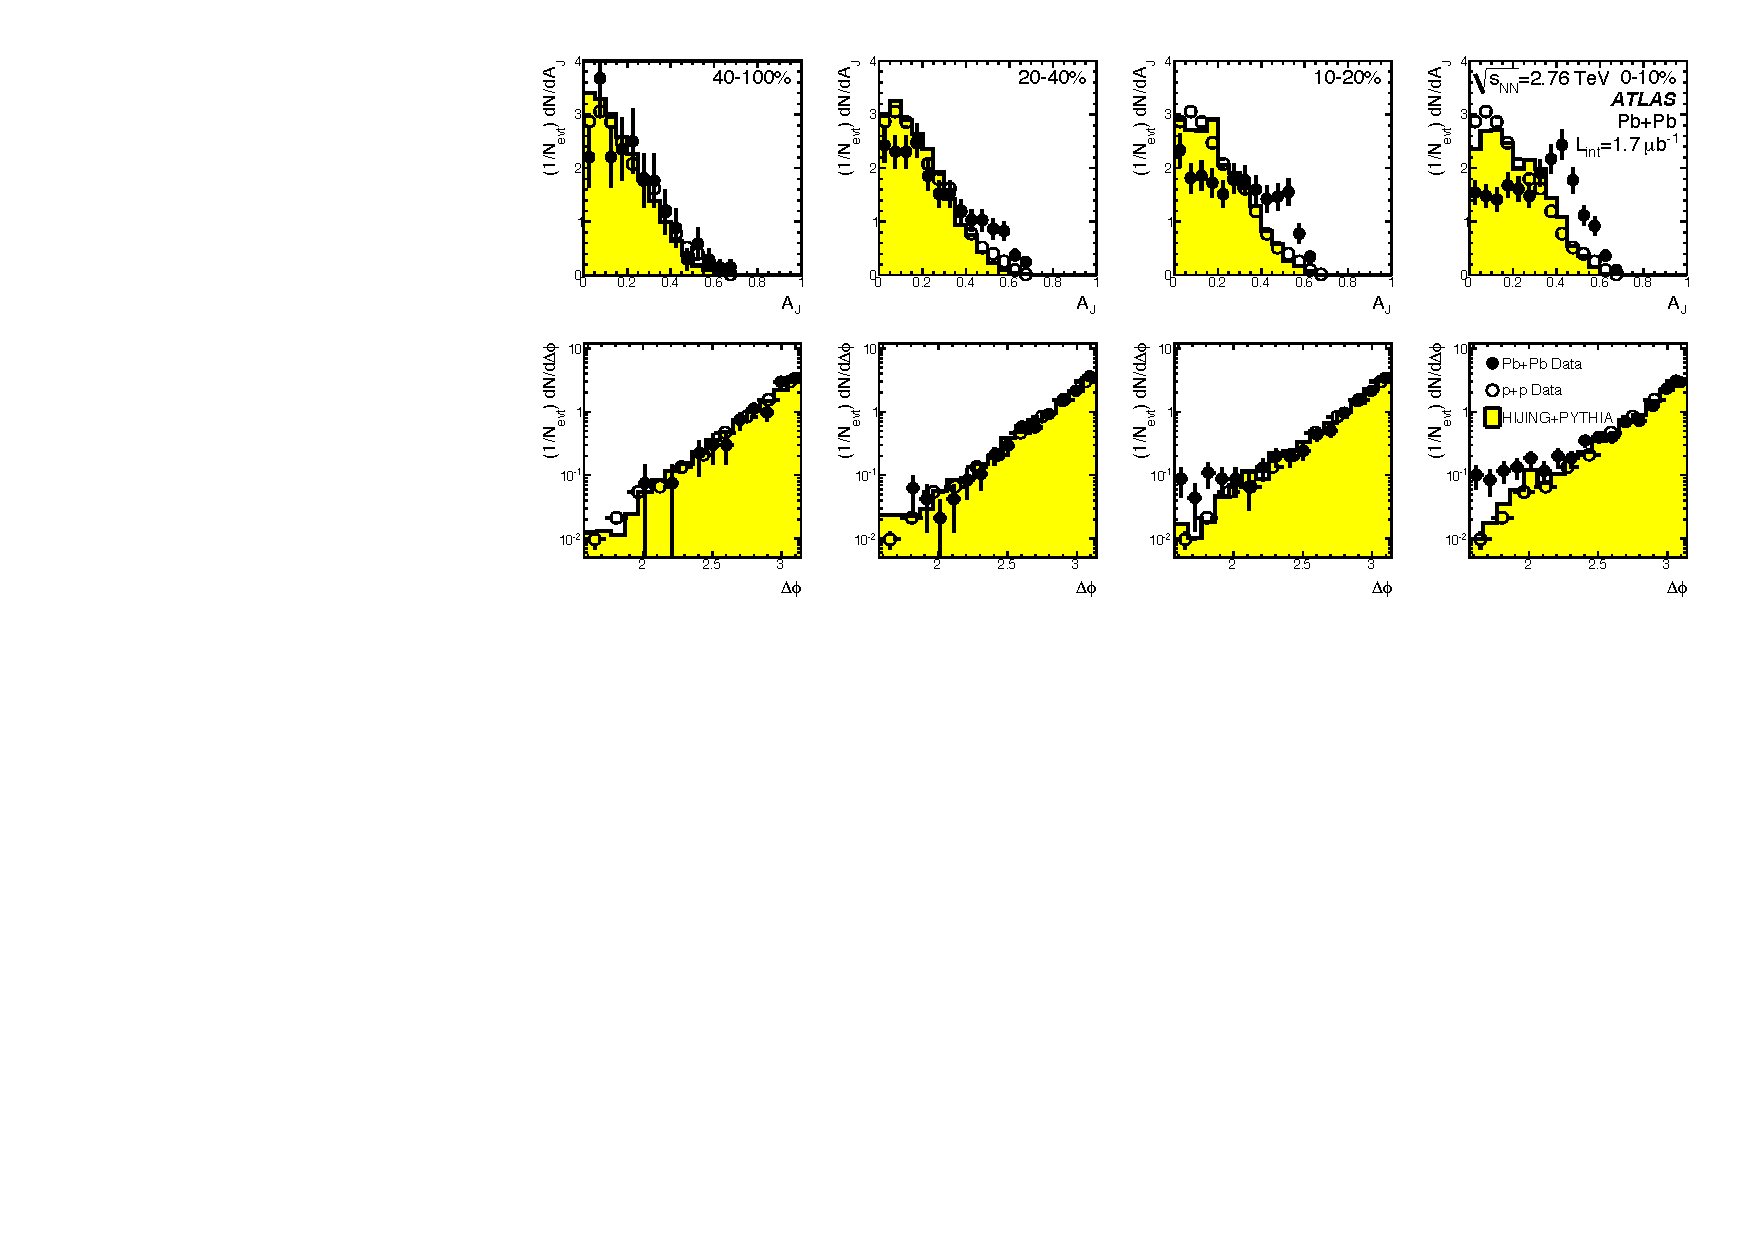
\includegraphics[width=0.8\textwidth]{jetfigures/final_4x2_23_newpp.pdf}
\caption{
(top) Dijet asymmetry distributions for data (points) and {\sc{hijing+pythia}} 
simulations (solid yellow histograms), as a function of collision centrality.  
Proton-proton data from $\sqrt{s}=7$\TeV\ is shown as open circles.
(bottom) Distribution of $\dphi$ between the two jets, 
for data and {\sc{hijing+pythia}}, shown in four bins of centrality.
Reproduced from~\cite{Aad:2010bu}.
}
\label{fig:pas:final_4x2}
\end{center}
\end{figure}

CMS extended this study using the higher-statistics 2011 Pb+Pb dataset~\cite{CMS_dijet} 
(with nearly a
factor of 100 increase in luminosity relative to the original ATLAS paper).
%Their result shows the evolution of $\langle p_{T,2}/p_{T,1} \rangle$, 
%using events with jet $p_{T1} > 120$ GeV, jet $p_{T,2} > 30$ GeV
%and $\Delta\phi_{12} > 2\pi/3$ to select back-to-back topologies, is shown in Figure~\ref{fig:PAS:CMS_pt_ratio}
%as a function of $p_{T,1}$.
%Since these data do not unfold the effect of the known experimental energy resolution for jets,
%they are compared to similarly reconstructed pp data as well as fully-reconstructed HYDJET events
%with embedded PYTHIA dijets.
%The rising trend observed in each panel, both the heavy ion and pp data, as well as the simulated events,
%can be generally understood as arising from the $\pT$ dependence of the jet resolution, which degrades at lower
%jet $\pT$, and thus pushes the reconstructed $\langle p_{T,2}/p_{T,1} \rangle$ lower simply from the 
%ordering of the jets.
%However, the difference between data and simulation increases significantly as the events become more
%central.  This is shown in the lower panels as a function of $p_{T,1}$ and is found to be constant within
%experimental uncertainties.

%\begin{figure}[!th]
%\begin{center}
%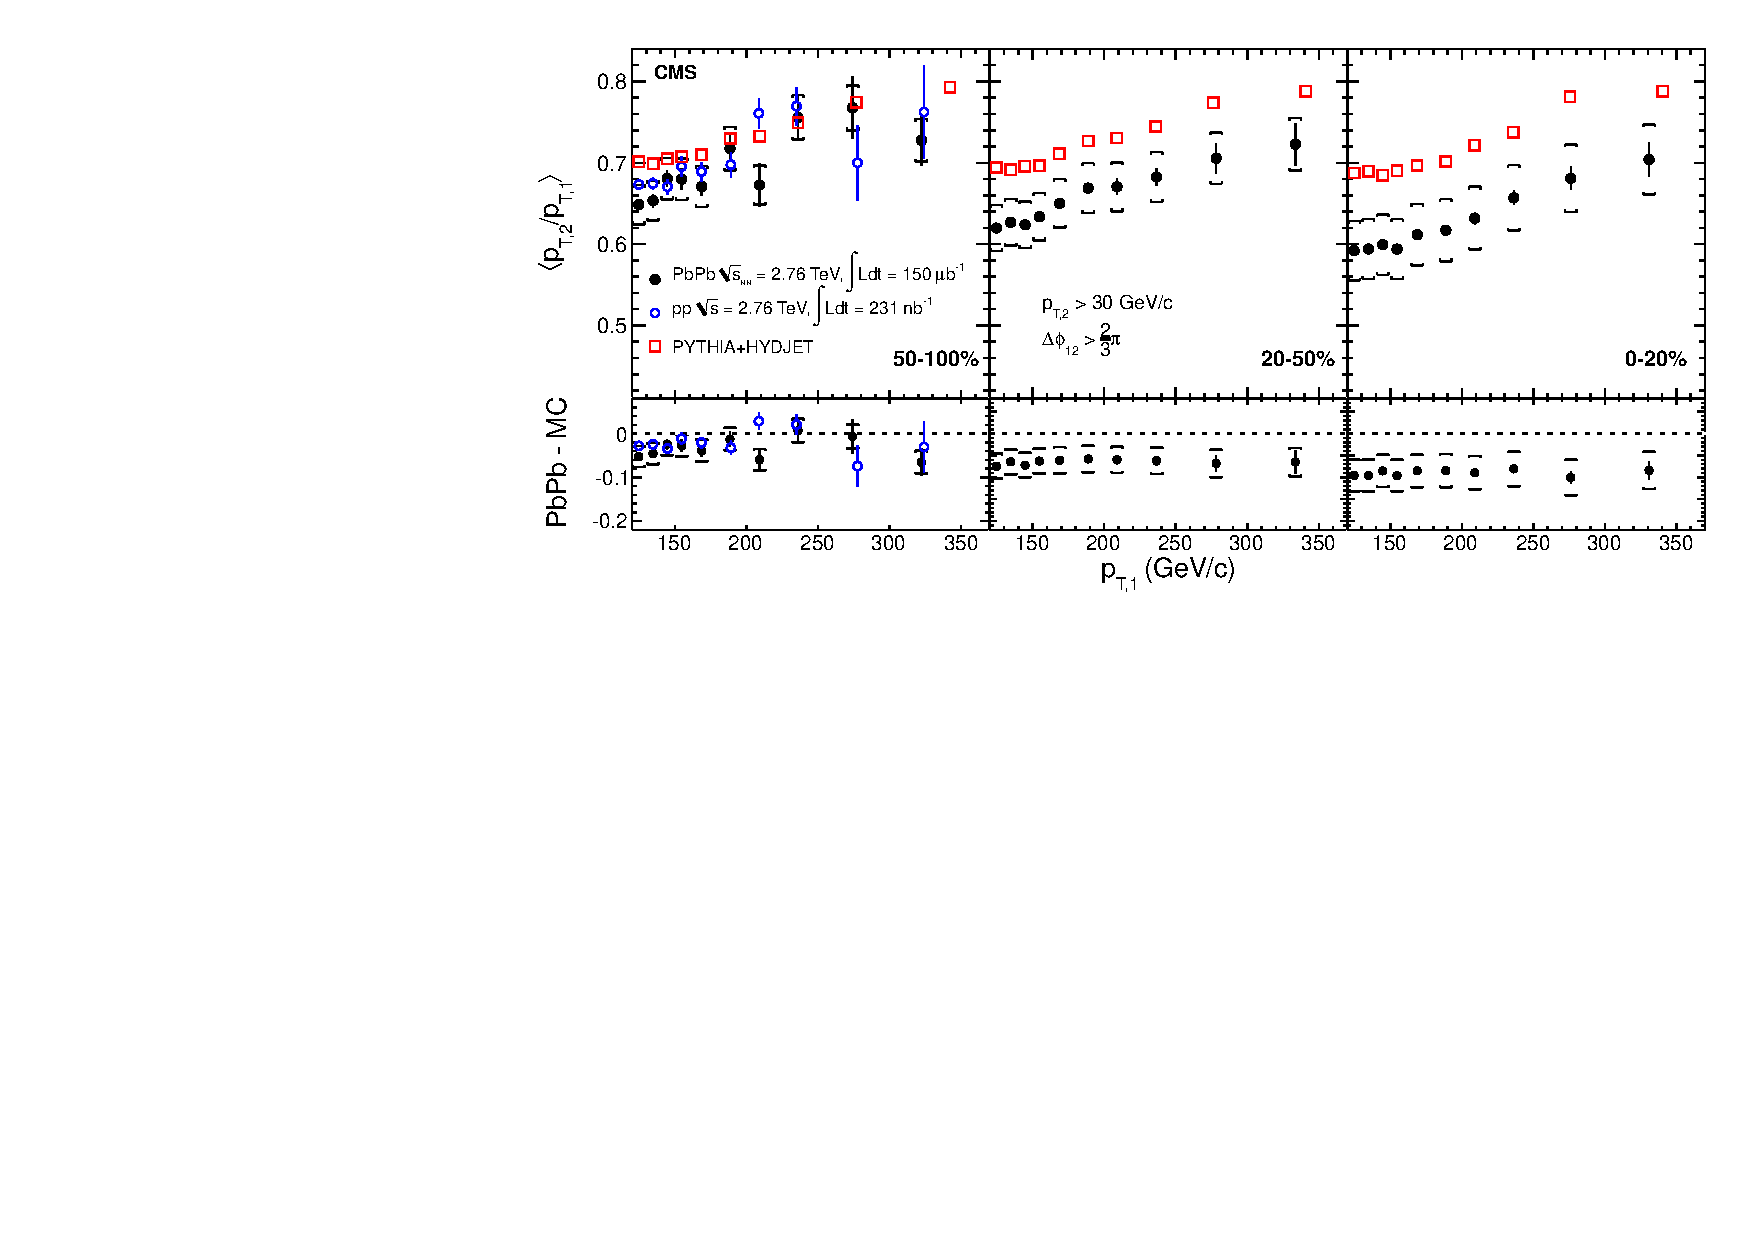
\includegraphics[width=0.75\textwidth]{jetfigures/deltaPtOverPt5_lead120_sub30_diff_20120103.pdf}
%%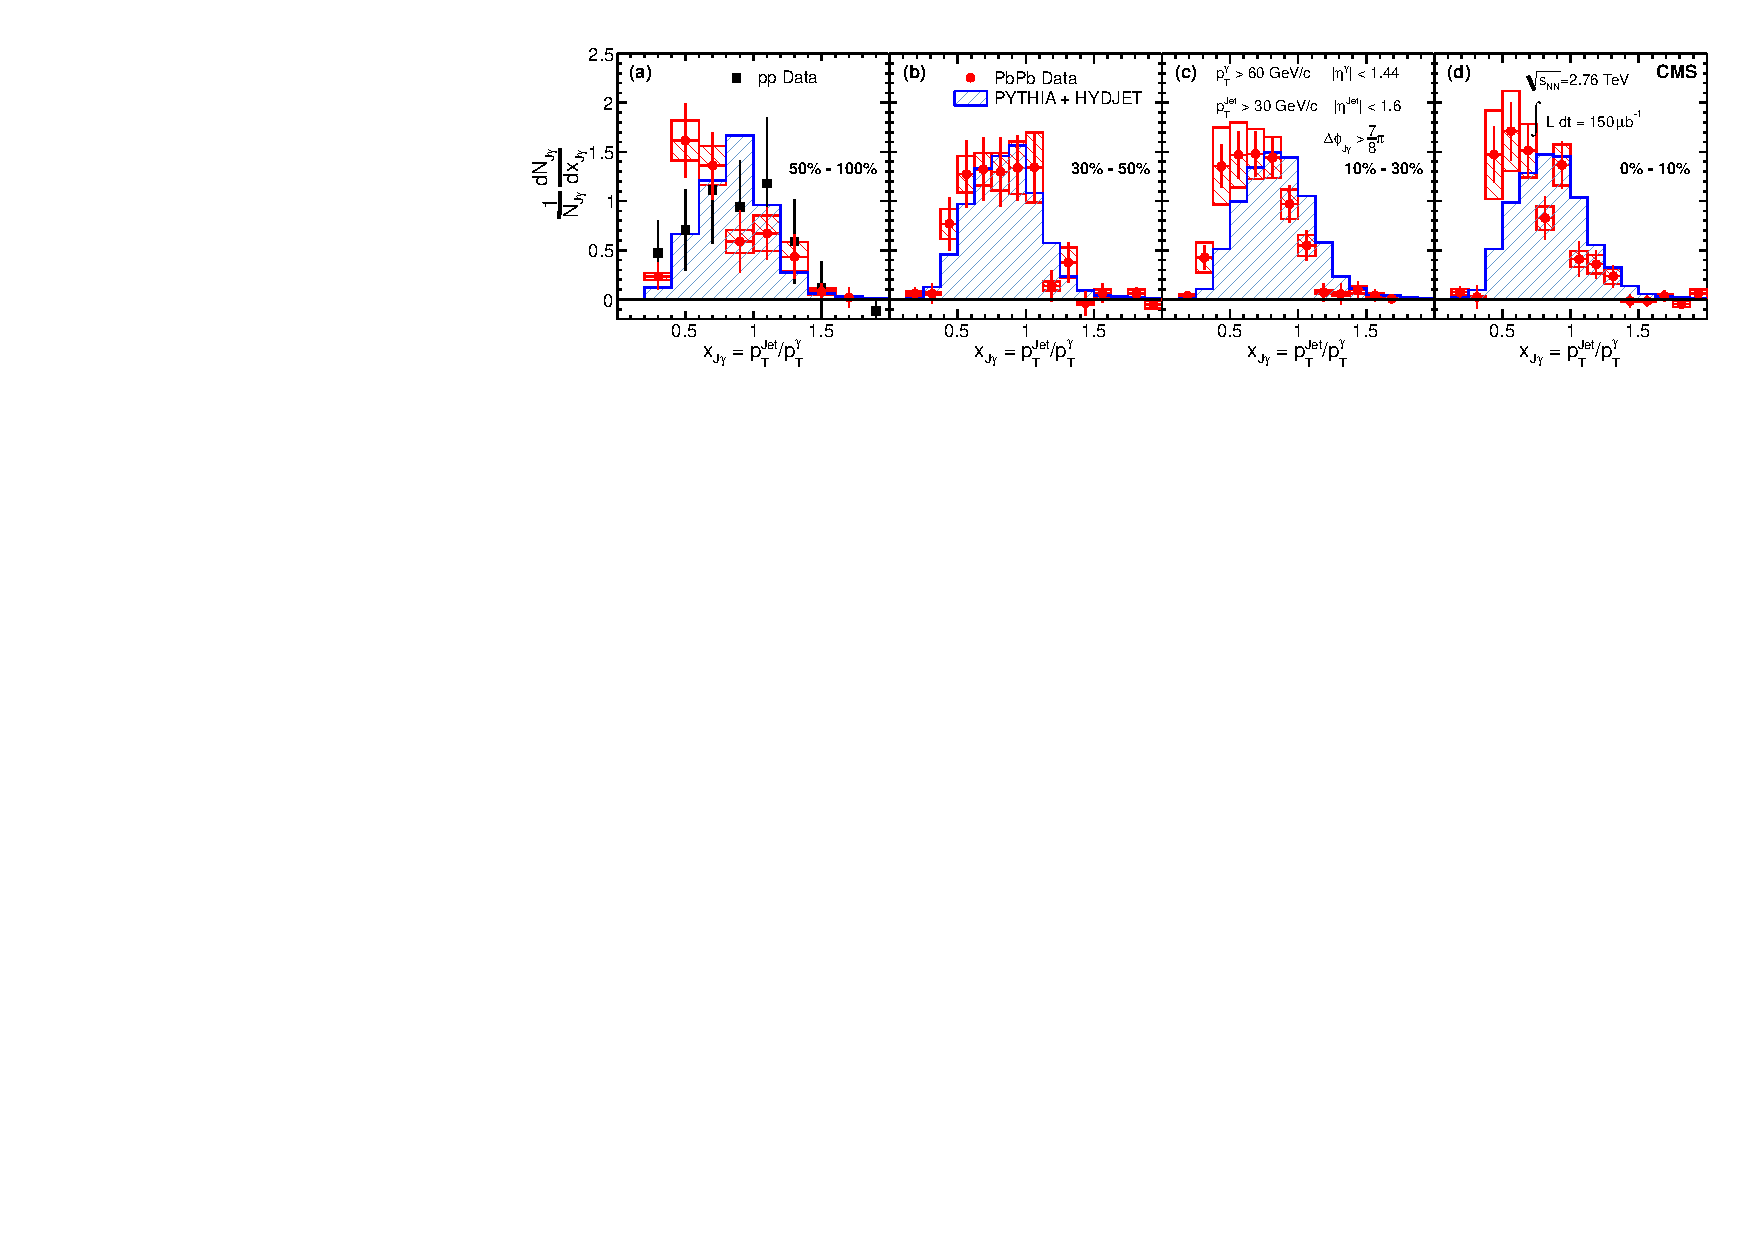
\includegraphics[width=0.75\textwidth]{jetfigures/Photonv7_Paper_InclPtRatio_all_cent4_G60J30_subDPhi1SS1_Isol0_Norm1log1.pdf}
%\caption{
%(top, upper): Dijet momentum ratio $\langle \ptsub/\ptlead \rangle$ as a function of
%leading jet \pT\ in three bins of collision centrality.
%\PbPb\ data are shown as points, with brackets indicating systematic uncertainties.  
%\PYTHYD\ calculations are shown as squares. In the peripheral bin,
%\pp\ data are displayed as open circles.
%(top, lower): Difference of $\langle \ptsub/\ptlead \rangle$ between the \PbPb\ results and \PYTHYD\ reference.
%Reproduced from~\cite{CMS_dijet}.
%(bottom)
%Distribution of the photon/jet 
%momentum ratio, \xjg, in four bins of collision centrality. 
%  The distributions are normalised to unit area. All panels compare
%\PbPb\ data (filled circles) to \pp\ data at
%  2.76\TeV\ (filled squares), and to the \PYTHYD\ MC simulations
%  (shaded histogram). Error bars show the statistical uncertainties and
%boxes show the (anti-correlated) systematic uncertainties. Reproduced from~\cite{Chatrchyan:2012gt}.
%}
%\label{fig:PAS:CMS_pt_ratio}
%\end{center}
%\end{figure}


\subsection{Jet yields and jet suppression}

While the dijet correlations were effective at demonstrating the presence of jet energy loss, 
they are in principle limited in their sensitivity to jet quenching physics by the fact that
there is no control over the energy loss of the leading jet.
This is certainly mitigated by the use of electroweak bosons in place of the leading jet,
for which initial CMS data exists but with relatively low statistics.
A more direct means to access the physics of energy loss is with the suppression of single
jet yields relative to a sample in which one expects energy loss effects to be minimal.
Both proton-proton collisions and peripheral heavy ion events are both used as the reference,
the latter in principle including nPDF and isospin effects which are absent in pp.

The left panel of Figure~\ref{fig:pas:rcprfour} shows the suppression of jets in Pb+Pb
in central events relative to peripheral via the ratio $R_{CP}$
\begin{equation}
R_{CP} = \frac{dN_{C}/d\pT / N_{coll,C}} {dN_{P}/d\pT / N_{coll,P}}
\end{equation}
where $C$ indicates the 0-10\% most central events and $P$ indicates the 60-80\% centrality interval.
For a given jet radius (e.g. $R=0.4$ shown here), no signficant $\pT$ dependence is observed.
However, as the centrality is increased, the yield of jets becomes systematically more suppressed,
reaching approximately a factor of two suppresison in the 0-10\% centrality interval.

Within a given centrality interval, the study of jet rates as a function their angle relative 
to the event plane provides a means to study the path length dependence of jet quenching.
The right panel of Figure~\ref{fig:pas:rcprfour} shows measured values of $v_2$ as a function
of jet $\pT$, where $v_2$ is the amplitude of an observed $\cos(2\phi)$ modulation relative to
the event plane measued with the ATLAS forward calorimeters.  This ``elliptic'' modulation of
jet rates has already provided similar information as high $\pT$ hadrons, but without 
any effects from the non-perturbative jet fragmentation functions.

\begin{figure}[!th]
\begin{center}
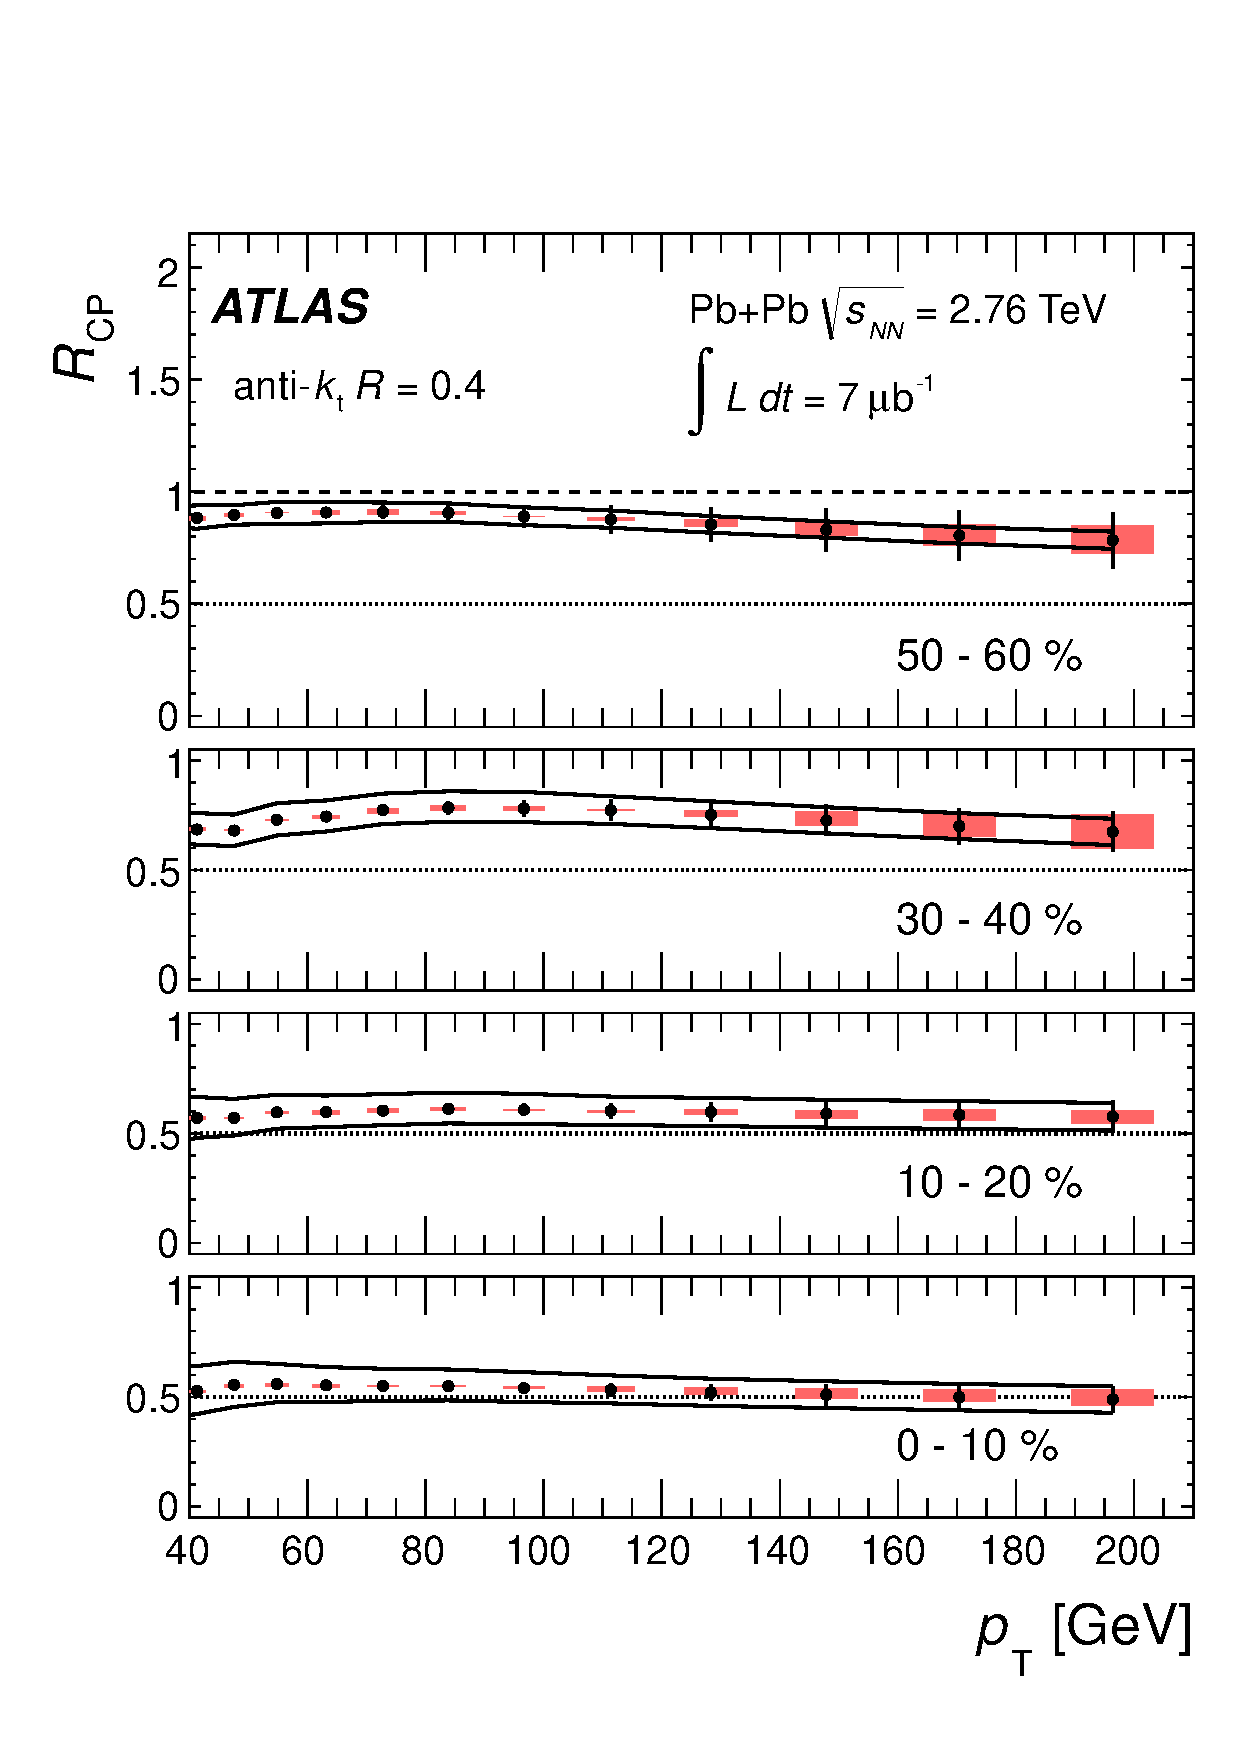
\includegraphics[width=0.4\textwidth]{jetfigures/ATLAS_jetRCP_04.pdf}
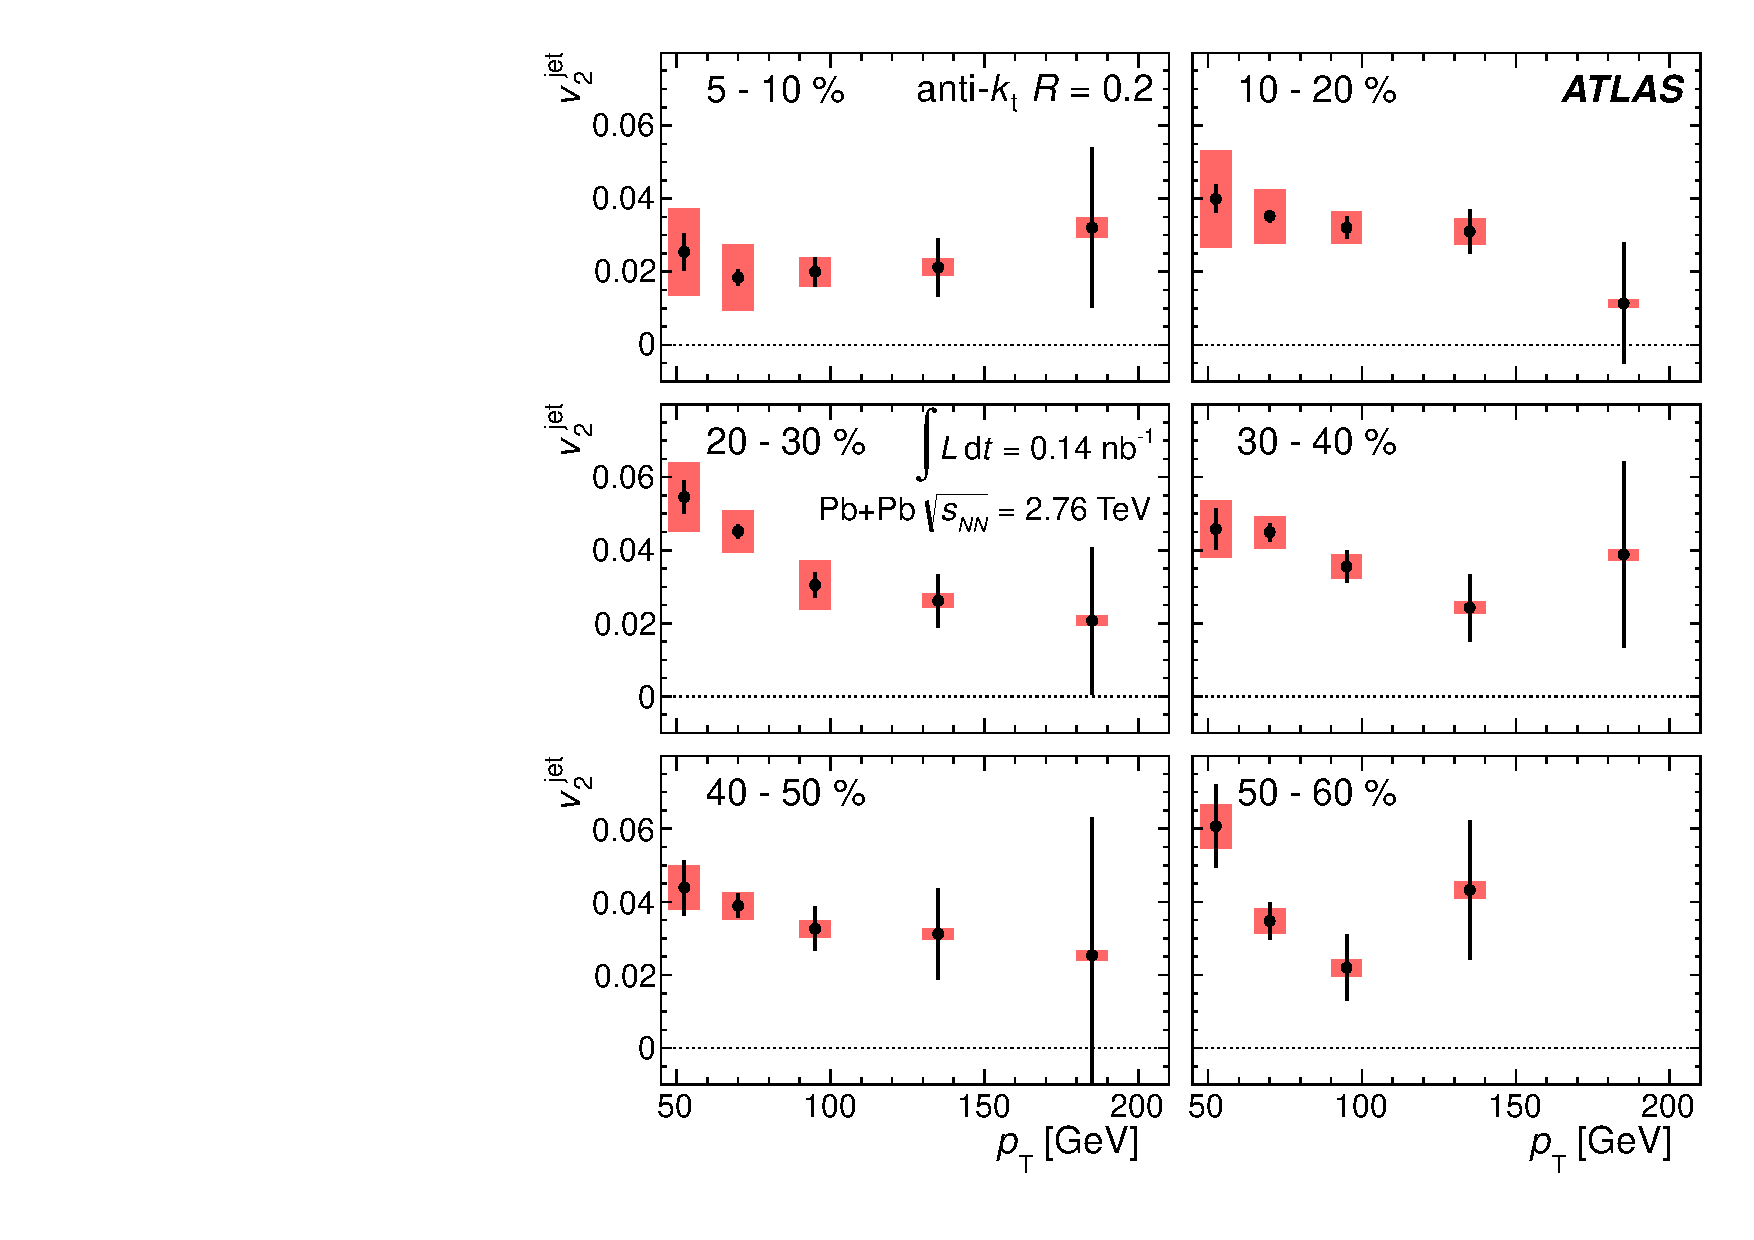
\includegraphics[width=0.49\textwidth]{jetfigures/ATLAS_jetv2.pdf}
\caption{
(left)\pT\ dependence of jet \Rcp\ for  $R=0.4$ jets,
in four bins of collision centrality. Error bars indicate
statistical errors while shaded boxes indicate
partially correlated systematic uncertainties. 
The solid lines show fully correlated uncertainties. 
Reproduced from~\cite{Aad:2012is}.
(right)\vtjet\ as a function of jet \pT\ in six bins of 
collision centrality.
Error bars indicate statistical uncertainties and 
systematic uncertainties are shown as shaded boxes. Reproduced from~\cite{Aad:2013sla}
}
\label{fig:pas:rcprfour}
\end{center}
\end{figure}

\subsection{Jet structure}

The study of both single and dijet jet rates clearly indicates that jets emitted in heavy ion 
collisions lose energy as they traverse the hot and dense medium.  It is natural to expect
that the radiation pattern emitted within a jet should be modified by the energy loss
process.  This has been addressed by a variety of approaches.

ATLAS has also measured the change in $R_{CP}$ as a function of jet radius (from 0.2 to 0.5) at
a fixed measured jet $\pT$.%  This is shown in Figure~\ref{fig:pas:ATLAS_jet_rcp}, where 
It is observed that the measured value of $R_{CP}$ increases significantly with increasing radius.
This indicates that jets with larger radius are slightly less suppressed, presumably since 
the jet energy profile is slightly wider in more central events.
%\begin{figure}[!th]
%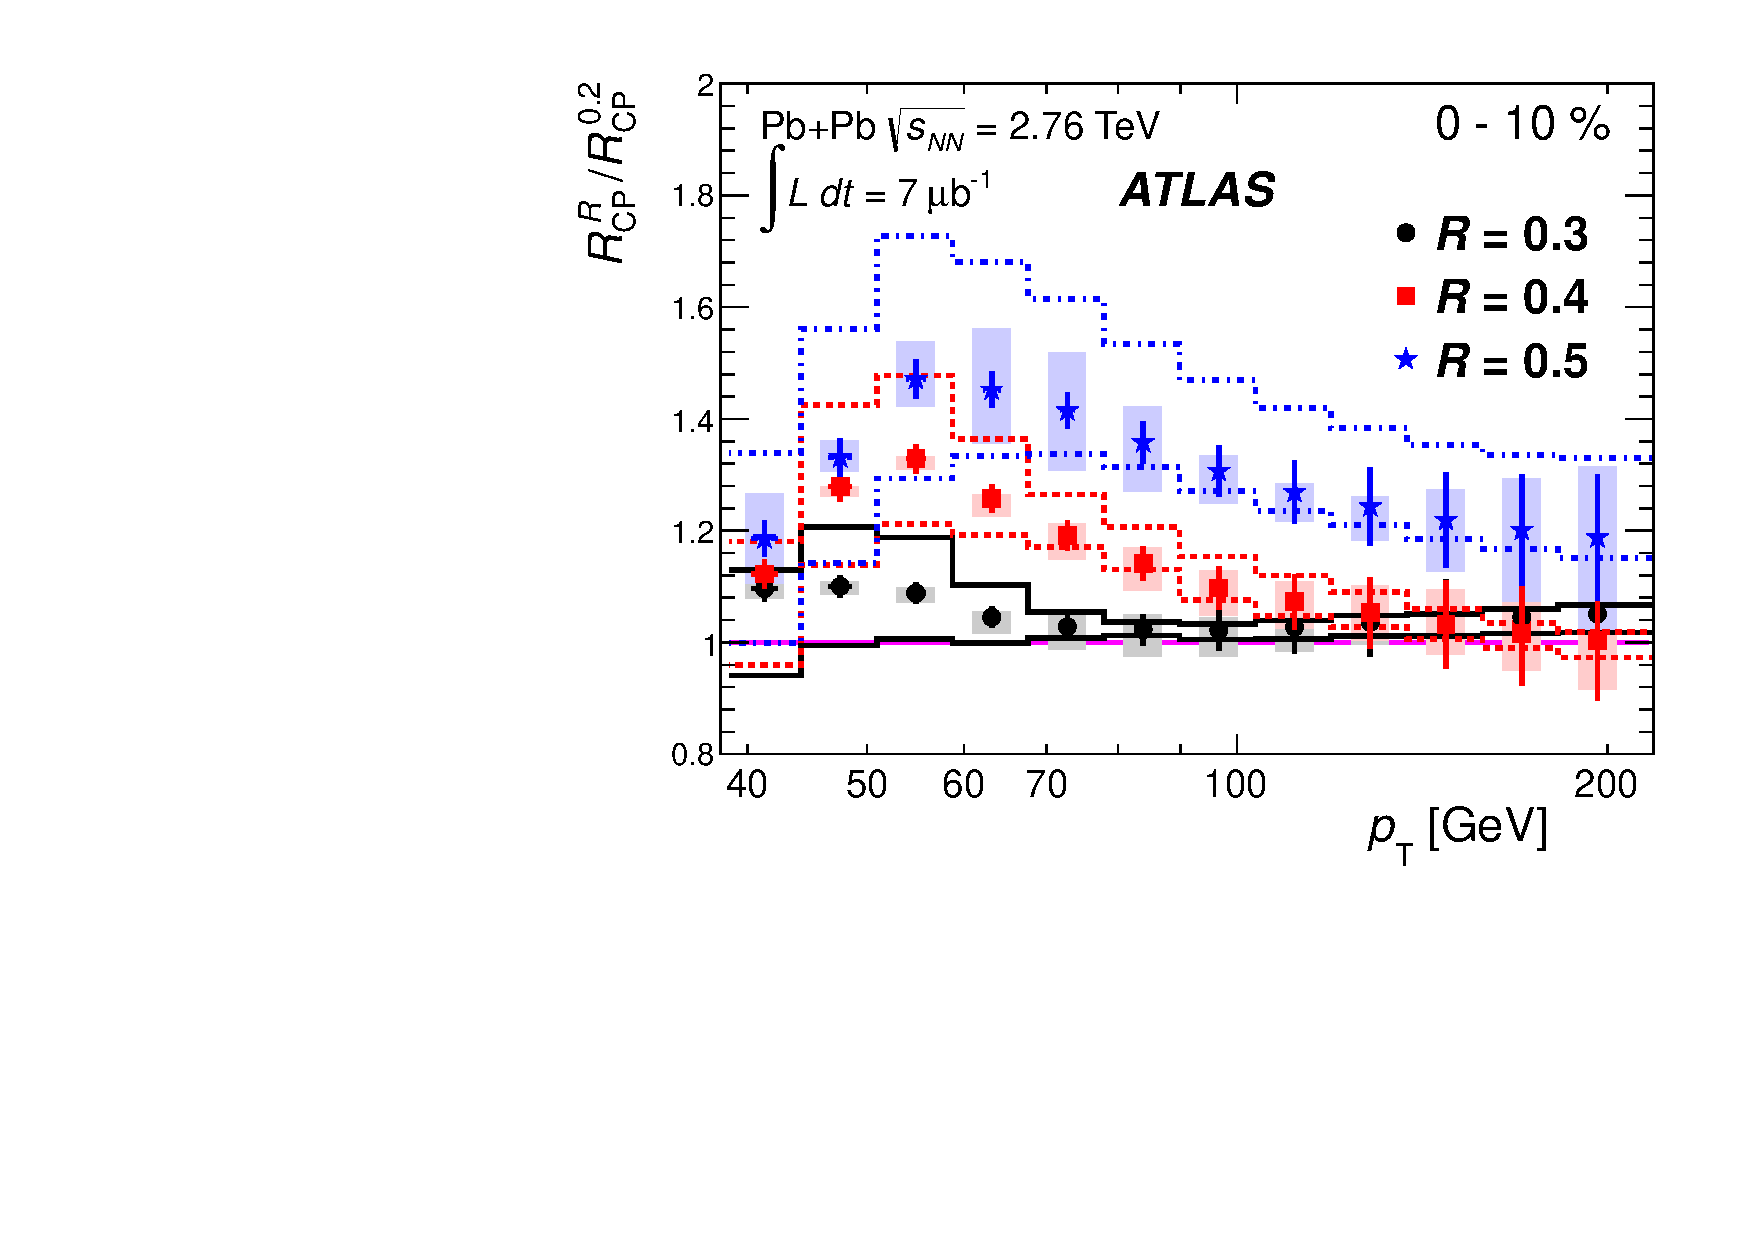
\includegraphics[width=0.59\textwidth]{jetfigures/ATLAS_jetRCP_size.pdf}
%\begin{center}
%\caption{
%Ratios of \Rcp\ values between $R = 0.3, 0.4$ and 0.5 jets and $R =
%0.2$ jets as a function of \pT\ in the 0--10\% centrality bin. The
%error bars show statistical uncertainties. The shaded boxes
%indicate partially correlated systematic errors. The lines indicate
%systematic errors that are fully correlated between different \pT\ bins.
%Reproduced from~\cite{Aad:2012is}.
%}
%\label{fig:pas:ATLAS_jet_rcp}
%\end{center}
%\end{figure}
%
The jet shape variable reflects the distribution of energy as a function of the radial coordinate
relative to the nominal jet direction.
The CMS measurements of jet shape as a function of centrality are shown in Figure~\ref{fig:pas:CMS_shape}.
The distributions for each system are individually normalized to unity.
The individual measurements in Pb+Pb and pp are shown as a function of centrality in the top row,
while their ratio is shown in the bottom row.
It is observed that the jet shape in peripheral collisions are consistent within uncertainties with pp,
while in the most central collisions, there is a depletion at moderate $r$ and an enhancment at large $r$.
While the relative enhancement at $r=0.3$ is large, it should be noted that the absolute change in the energy
flow is not large.

%The longitudinal fragmentation function $(1/N_{jet}) dN_{tr}/d\zeta$, where $\zeta = \ln(1/z)$ with
%$z = \p^{track}_{||}/p_{jet}$, measured in the dijet center-of-mass frame was 

\begin{figure}[!ht]
\begin{center}
%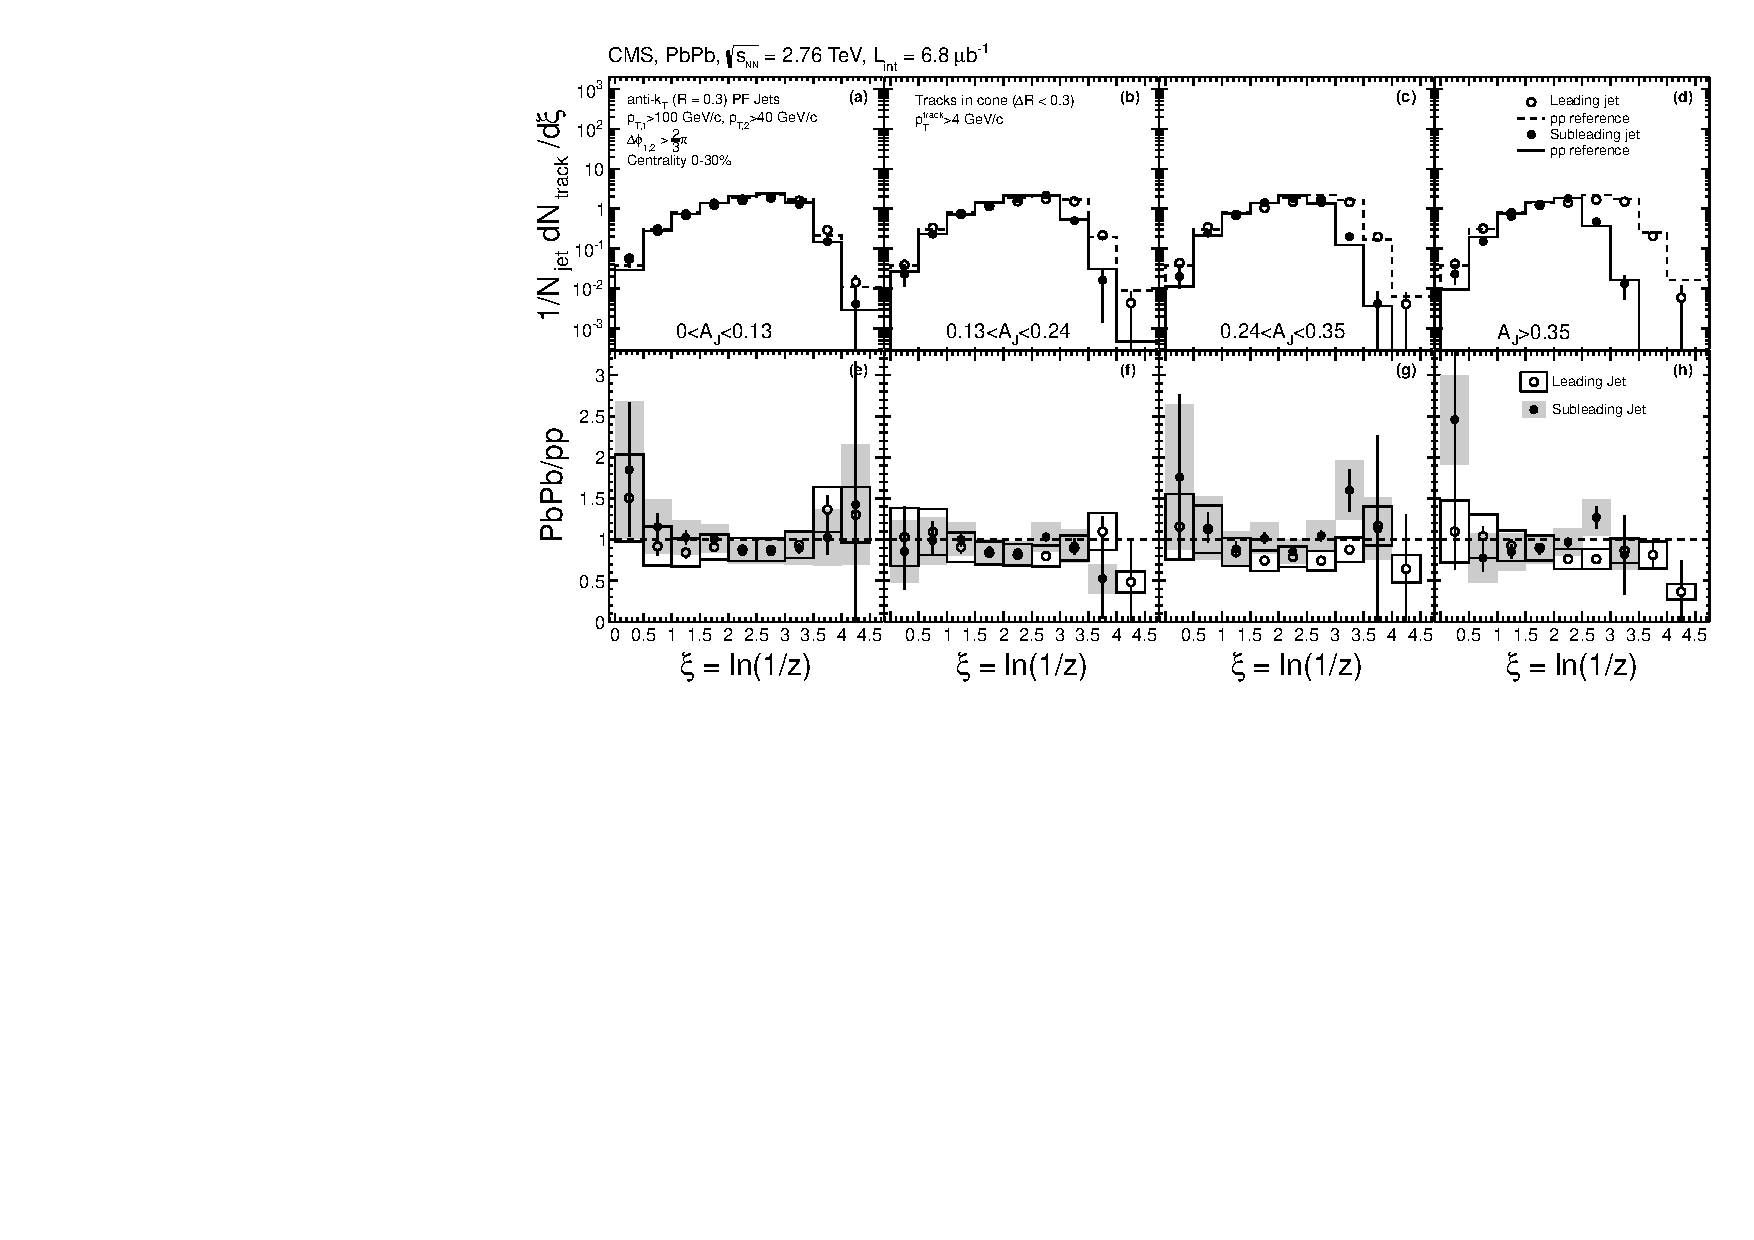
\includegraphics[width=0.8\textwidth]{jetfigures/xsi_div_both_effv9_l100s40_0to12_dphi20eta20dr3pt4id1_cwt_ppDiv_gray.pdf}
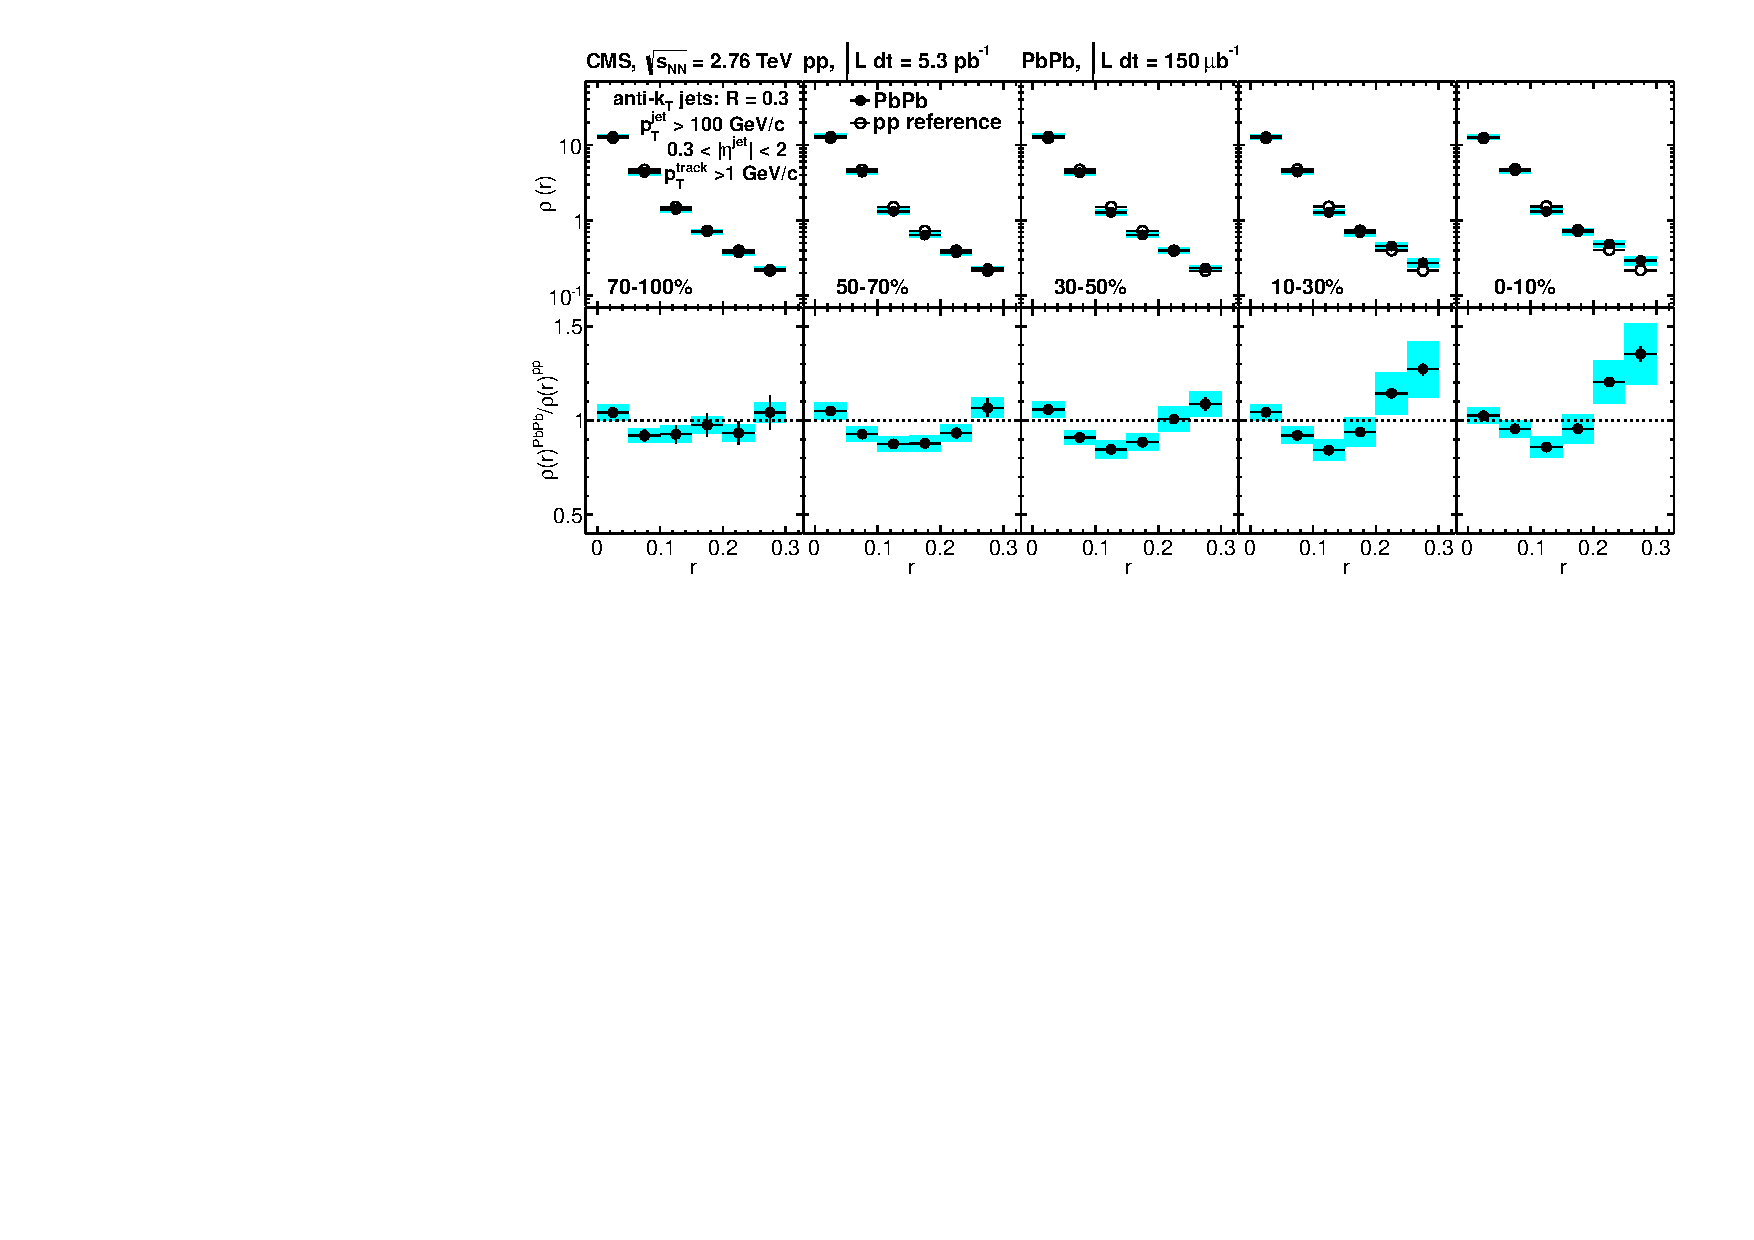
\includegraphics[width=0.8\textwidth]{jetfigures/cms_shape_Figure2.pdf}
\caption{
%(top)
%(a--d) Fragmentation functions for the leading (open circles) and subleading (solid points) 
%jets in four regions of $\AJ$ in central \PbPb\ collisions compared to the \pp\ reference.
%(e--h) Ratio of each fragmentation function to its \pp-based reference.
%Error bars shown are statistical. The systematic uncertainty is
%represented by hollow boxes (leading jet) or gray boxes (subleading jet).
%(i--l) Jet $\pT$ distributions in \PbPb\ collisions in four regions of $\AJ$
%compared to a \pp-based reference. Only statistical uncertainties are shown.
%Reproduced from~\cite{Chatrchyan:2012gw}.
%
(upper): Differential jet shapes in \PbPb\ collisions (filled circles)
as a function of distance from the jet axis for inclusive jets with $\pT^{\mbox{jet}} >100\GeVc$
in five bins of centrality.  The \pp-based reference is shown with open symbols.
The shaded regions represent the \PbPb\ systematic uncertainties.
Statistical uncertainties are smaller than the marker size.
(lower): Jet shape ratios $\rho(r)^{\PbPb}/\rho(r)^{\pp}$.
Error bars show the statistical uncertainties and shaded boxes indicate the systematic uncertainties. 
Reproduced from~\cite{Chatrchyan:2013kwa}
}
\label{fig:pas:CMS_shape}
\end{center}
\end{figure}

\subsection{Energy flow in dijet events}

The previous sections have demonstrated that the energy loss of jets is accompanied by a modest
change in jet structure within the nominal jet cone, suggestive of a broadening of the overall
jet energy flow.
Given this, it remains an open question where the rest of the lost energy goes.  
In the first CMS jet publication, the overall conservation of transverse momentum was used to 
study the energy flow associated with asymmetric dijets.  By using all tracks with $\pT>0.5$ GeV,
it was found that there was no missing transverse energy within the angular acceptance of the
CMS silicon tracker.  
The transverse energy balance was then compared in data and simulations 
for $\Delta R<0.8$ and $\Delta R >0.8$ as a function of the dijet asymmetry.
The most asymmetric events in the simulations achieved the overall energy balance 
with high momentum particles, suggesting that the balance at large angle was still achieved
by jet emission.  In the data, the energy balance was achieved by the emission of more 
soft particles, quite different than the simulations.

\begin{figure}[!ht]
\begin{center}
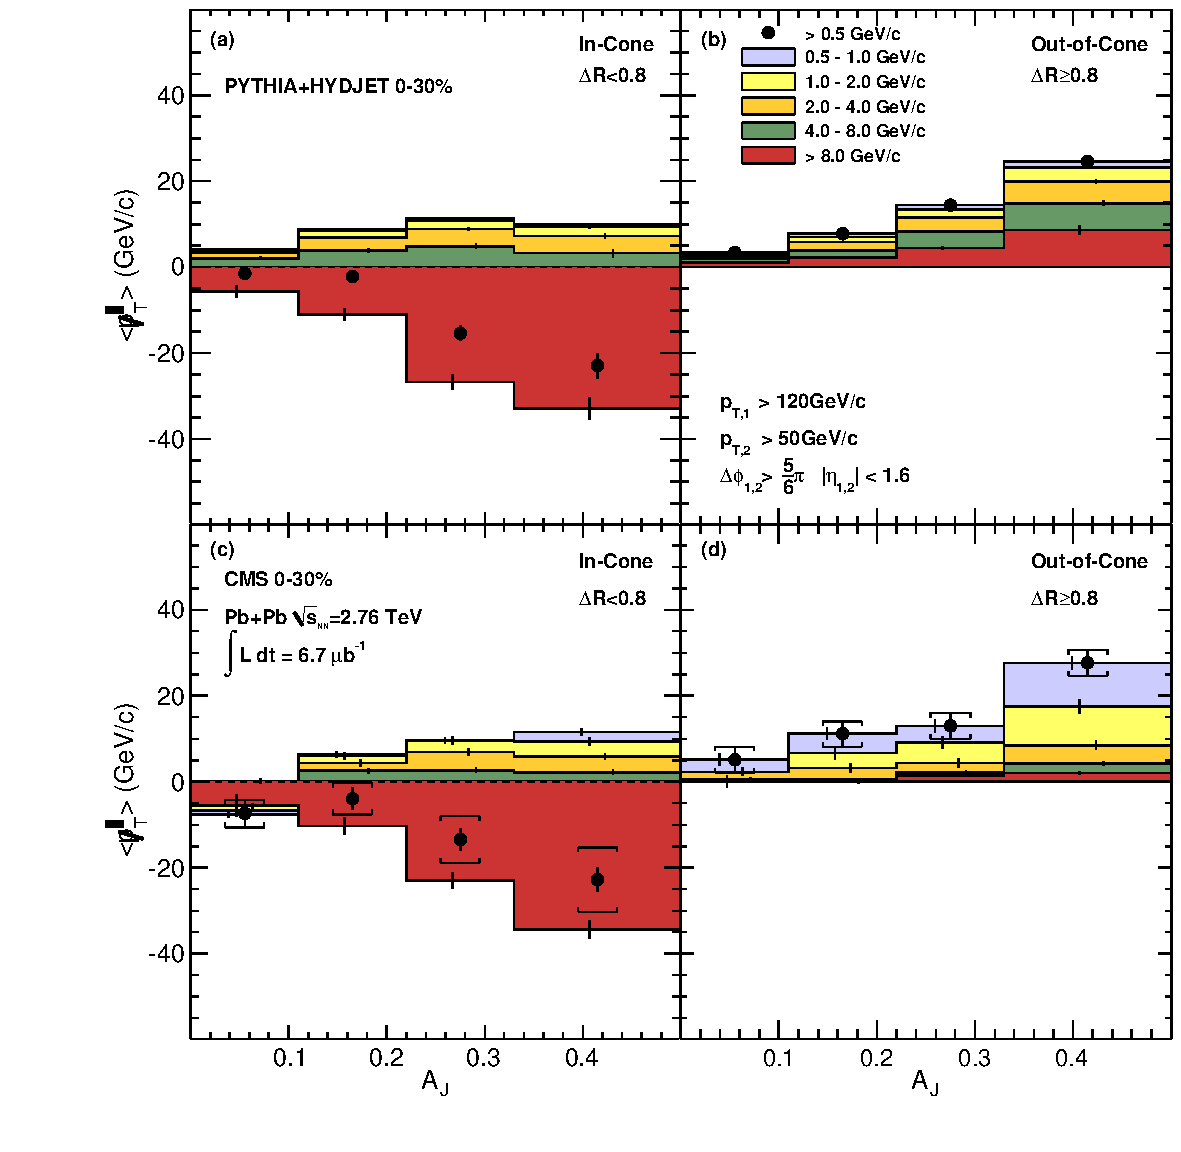
\includegraphics[width=0.5\textwidth]{jetfigures/missingPtParallel-Corrected-data-InConeOutConeDPhiCut_ntv6_2.pdf}
\caption{Average missing transverse momentum,
$\langle \displaystyle{\not} p_{\mathrm{T}}^{\parallel} \rangle$,
for tracks with $\pT > 0.5$\GeVc, projected onto the leading jet axis (solid circles).
The $\langle \displaystyle{\not} p_{\mathrm{T}}^{\parallel} \rangle$ values are
shown as a function of dijet asymmetry
$A_J$ for 0--30\% centrality, inside ($\Delta R < 0.8$) one of the leading or subleading jet cones (left) and
outside ($\Delta R > 0.8$) the leading and subleading jet cones (right).
For the solid circles, vertical bars and brackets represent
the statistical and systematic uncertainties, respectively.
For the individual $\pT$ ranges, the statistical uncertainties are shown as vertical bars.
Reproduced from~\cite{Chatrchyan:2011sx}.}
\label{fig:GR:CMS_missingpT}
\end{center}
\end{figure}



\section{SUMMARY AND OUTLOOK}
\label{summary}
This article attempts to overview the studies of hard-probes observables exploiting data from the first two runs with Pb--Pb collisions at the CERN LHC, running at the collision energy $\rootsNN = 2.76$~TeV per a nucleon pair. Each of the three major LHC experiments (ALICE, ATLAS and CMS) sampled an integrated luminosity in excess of 100~$\mu$b$^{-1}$, corresponding to about a billion of minimum-bias Pb--Pb collisions. The suppression of high-\pT\ particles, relative to what is measured in proton--proton collisions, is expressed with the \pt\ dependence of the nuclear modification factor \Raa. This reveals a strong suppression at intermediate \pT\ (6--8~GeV), but then a lesser effect, and even a plateau for \pt\ above 40~GeV, with a \Raa\ value of about 0.5--0.6, very similar to that found for jet suppression. The study of identified-particle suppression shows a presence of three \pt\ regions: bulk ($\pt < 2$--$3$~GeV), intermediate (up to 7--8~GeV), and fragmentation (above that); and demonstrates that probably there is no any particle-identified life above \pt\ of 10~GeV. Two particle correlations, despite not being a full jet measurement, provide an insight into the suppression in the away-side region and an enhancement on the near-side,
suggestive of modified in-medium fragmentation.

Heavy flavor, copiously produced at the LHC, is expected to show different energy loss than that of
light quarks and gluons. Early results show a strong suppression of D mesons, comparable with that for light-flavor hadrons. The B-meson production, measured with J$/\Psi$ from B-meson decays, indicates less suppression for beauty compared to charm quarks. Thus, for the first time, the predicted mass-quenching hierarchy is respected. The J$/\psi$ yield is found to be suppressed over a wide rapidity range, although demonstrating qualitatively different centrality behavior compared to RHIC results. The \Jpsi\ suppression at low $\pT$ is largely less than that measured at RHIC, suggesting clearly a new production mechanisms. Models, invoking regeneration processes due to the large charm-quark densities at the LHC, are likely to explain this phenomena. Both, D mesons and \Jpsi, show an azimuthal asymmetry demonstrated with a non-zero $v_2$, which is an indication for charm-quark thermalization. The $\Upsilon$ family confirms the predicted behavior in heavy-ion collisions, with all states being suppressed relative to pp collisions, and the more weakly bound higher states showing stronger suppression than the more tightly bound \PgUa\ state.

The particle production involving hard processes is well calibrated using measurements of electro-weak bosons, such as W and Z, as well as direct photons. All of these particles are found to have cross sections consistent with perturbative QCD calculations scaled by the number of binary collisions, $N_{\rm coll}$. In this context, the modifications of jet yields in (semi-)central heavy-ion collisions can clearly be attributed to the energy loss of partons traversing the hot, dense medium. The jet energy loss has been addressed using several techniques, from dijet $E_{\rm T}$ imbalance to single-jet suppression, both inclusive and differentially in $\varphi$. Jet fragmentation
in heavy-ion collisions has also been measured and found to be modified, especially at large angles with respect to the jet axis. The jet--direct-$\gamma$ correlations shows a similar energy loss effect.

The results presented here are mainly those already published, and many more results are in preparation. Therefore, this review should be seen as a snapshot of the state of the field. The wealth of results from the first two heavy-ion runs, and the upcoming running at higher energy ($\energy = 5.1$ TeV) and luminosity exceeding the design value of $10^{27}$~cm$^{-2}$s$^{-1}$, should provide even deeper insight into the nature and properties of the hot and dense matter formed in nuclear collisions at the LHC.

The progress towards a detailed characterization of this strongly-interacting medium will focus more on hard probes,
studying their interactions with this medium, and on hadronization. These will include measurements of heavy-flavor particles, quarkonium states, real and virtual photons, jets and their correlations with other probes (in particular electro-weak bosons). The production rate of all these processes are significantly larger at the LHC than at previous accelerators. In addition, the interactions with the medium of hard probes is better controlled theoretically than the propagation of soft light partons.

In order to achieve these goals, high precision measurements together with high integrated luminosities
are required. This will give an access to the rare physics channels needed to understand the dynamics of this condensed phase of QCD matter. Therefore, the LHC collaborations are upgrading the current detectors to enhance their vertexing capabilities, and to allow for data taking at substantially higher rates.  The upgrade strategy for
heavy-ion running is formulated under the assumption that, after the second long shutdown in 2018--19, the LHC will progressively increase its luminosity also with Pb beams, eventually reaching an interaction rate of about 50~kHz, corresponding to the luminosity $6 \times 10^{27}$~cm$^{-2}$s$^{-1}$. The proposed plan~\cite{ALICEUpgradeLoI}
envisage to accumulate 10~nb$^{-1}$ of Pb--Pb collisions inspecting ${\cal O}(10^{10})$ interactions, which is necessary to address the proposed physics programme, focused on hard probes, both at low- and high-\pt, as well as on the multi-dimensional analysis of such probes with respect to centrality, event plane, and multi-particle correlations. 

\section*{ACKNOWLEDGMENT}
\label{acknowledgment}

\bibliography{heavyion}

\end{document}
